% Wczytanie szablonu
\documentclass[nostrict]{Szablon}

% Definicja dokumentu
\usepackage[unicode=true]{hyperref}
\usepackage{listings}
\newcommand\PDFtitle{Tytuł pracy}
\newcommand\PDFauthors{Imie Nazwisko}
\hypersetup{
  pdftitle={\PDFtitle},
  pdfauthor={\PDFauthors},
}

\addbibresource{bib.bib}

% Zmiana czcionki dla symulacji maszynopisu (verbatim)
\makeatletter
\renewcommand{\verbatim@font}{\ttfamily\small}
\makeatother

% Część właściwa pracy
\begin{document}
\chapter*{Streszczenie}
\addcontentsline{toc}{chapter}{Streszczenie}  

\chapter*{Abstract}
\addcontentsline{toc}{chapter}{Abstract}  

\chapter*{Spis treści}
\addcontentsline{toc}{chapter}{Spis treści}

\tableofcontents

\chapter*{Wykaz ważniejszych oznaczeń i skrótów}
\addcontentsline{toc}{chapter}{Wykaz ważniejszych oznaczeń i skrótów}


\chapter{Wstęp i cel pracy}\label{chap:introduction}

Celem projektu jest zaprojektowanie oraz zaimplementowanie gry real-time strategy osadzonej we wczesnym średniowieczu i przeznaczonej dla jednego gracza. Kluczowe dla niej będzie uwzględnienie mechanik, które umożliwią użytkownikowi podejmowanie decyzji w zbliżony sposób to tego wykorzystywanego w tamtych czasach. Dawniej decyzji strategicznych nie podejmowano na podstawie precyzyjnych map. Ludzie zmuszeni byli  budować  przestrzenny obraz istniejącej sytuacji  w toku dyskusji z naocznymi świadkami, takimi jak dowódcy czy podróżnicy. Z punktu widzenia projektu, uwzględnienie tych różnic jest kluczowe, gdyż umożliwi to graczowi wczucie się w realia epoki. Bliski pożądanemu efektowi jest sposób w jaki zrealizowano dowodzenie drużyną w grze RPG „Pillars of Eternity”. Niestety, te mechaniki w tego typu grach zwykle są bardzo ograniczone i nie pozwalają na zarządzanie większymi grupami wojsk, czy budowę baz, czyli zagadnienia podstawowe z punktu widzenia gier RTS. Z tego powodu celem pracy jest opracowanie projektu gry strategicznej czasu rzeczywistego dla jednego gracza, w której dowodzenie przebiegałoby w sposób możliwie zgodny z realiami historycznymi.

\chapter{Przegląd strategii czasu rzeczywistego}

W niniejszym rozdziale zostały przedstawione wybrane mechaniki wykorzystywane w grach typu RTS. Omówione zostało ich
działanie na podstawie przykładów z wybranych gier. Celem tego jest obrazowe zaprezentowanie ich integralności
w grach oraz wpływu na rozgrywkę.

Na odbiór gry wpływają zawarte w niej mechaniki. Twórcy bardzo częstostosują w nich uproszczenia, co ma na celu
ułatwienie graczowi wykonywanie zadań. Ma to jednak ogromny wpływ na zachowanie realizmu w grach, zwłaszcza tych opartych
na wydarzeniach historycznych oraz prawdziwym świecie.

\section{Przegląd wybranych gatunków gier komputerowych}
W niniejszym podrozdziale zostały przedstawione wybrane gatunki gier komputerowych, które są najistotniejsze z punktu widzenia
projektu. Przede wszystkim zostały opisane gry typu strategii czasu rzeczywistego oraz strategiczne gry turowe TBS (ang.
textit{turn-based strategy}. Ma to na celu zaprezentowanie podstawowych różnic pomiędzy tymi gatunkami.

"Gatunek określa graczowi, w jakiego typu grę będzie grał i jest bardzo przydatnym sposobem klasyfikacji gier"\cite{practical_game_design}.
Podział gier na gatunki pozwala na określenie podstawowych cech gry i daje ogólne pojęcie o jej charakterze. "Dlatego w
grach gatunek niesie więcej informacji niż temat i sceneria"\cite{practical_game_design}. Z tego powodu w celu
zrozumienia celu projektu ważne jest zrozumienie podobieństw i różnic pomiędzy kluczowymi dla niego gatunkami.

\subsection{Specyfika gier RTS (Bartosz Strzelecki)}\label{ss:rts}
Strategie czasu rzeczywistego RTS (ang. \textit{real-time strategy}) odróżnia się od innych gatunków występowaniem zarówno strategicznych, jak i taktycznych
elementów rozgrywki. Podstawowe założenia klasycznych gier RTS to skomplikowana równowaga pomiędzy zarządzaniem zasobami, budowaniem budynków oraz
dowodzeniem armii. Centralnym elementem rozgrywki RTS jest zarządzanie różnorodnymi jednostkami, z których każda posiada unikalne zdolności i rolę na polu bitwy.

Gry te działają w dynamicznym środowisku czasu rzeczywistego, co odróżnia je od strategii turowych TBS (ang.  \textit{turn-based stratrgy}). Ten model wymusza szybkie podejmowanie decyzji
i wymaga od gracza podzielności uwagi. Strategie czasu rzeczywistego zwykle też posiadają bardziej złożoną konstrukcję mapy, zawierającą skomplikowane
rozłożenia celów i przeszkód, natomiast mapy w strategiach turowych zazwyczaj wykorzystują ruch oparty o siatkę, co zapewnia dużo bardziej
zorganizowane środowisko rozgrywki.

W grach strategicznych czasu rzeczywistego w trybie kampanii zachowanie przeciwników jest zaprojektowane z myślą o zanurzeniu gracza w fabularnej opowieści, jednocześnie
prezentując wyzwania związane z rozgrywką. Akcje wykonywane przez sztuczną inteligencję są dostosowane do celów danej misji, co pozwala
na dopasowanie do obowiązującej narracji.

Tego typu produkcje pozwalają również na wciągającą rozgrywkę w trybie wieloosobowym, w którym gracze mogą rywalizować między sobą, jak również
współpracować w celu pokonania wspólnego przeciwnika kontrolowanego przez sztuczną inteligencję. Na ten styl rozgrywki jest nakładany istotny nacisk
w wielu grach tego gatunku, poprzez zapewnienie zróżnicowanych grywalnych frakcji, zachowując przy tym symetrię balansu rozgrywki.

Z uwagi na cechę gier gatunku RTS polegającej na ciągłym przepływie czasu, gracze są zmuszeni
do podejmowania szybkich decyzji w dynamicznie rozwijającej się sytuacji. Mijający czas
wywiera presję na użytkowników, wymagając natychmiastowej reakcji w podejmowanych decyzjach.
Z tego powodu w grach z tego gatunku efektywne zażądanie czasem jest kluczowym elementem
wymaganym do osiągnięcia oczekiwanych rezultatów. Zazwyczaj czas upływa w sposób jednostajny, oznacza to, że
nie mogą spowolnić lub zatrzymać tempa rozgrywki, aby odetchnąć lub przemyśleć swój plan działania.

Ogólnie rzecz biorąc, gatunek RTS oddaje dreszcz emocji związanych z prowadzeniem działań strategicznych, co wymaga połączenia zaradności,
przewidywania i sprytnego podejmowania decyzji na szybkim i stale zmieniającym się polu bitwy.
"Wewnątrz tej ogólnej definicji znajdują się pewne podgatunki. Jak wspomniano wcześniej, tradycyjne gry RTS składają się z elementów budowania bazy, zarządzania zasobami i drzew technologicznych. Do tej kategorii pasują gry takie jak Command \& Conquer, StarCraft i Age of Empires."\cite{stateoftherts}

Do gatunku gier strategii czasu rzeczywistego należą między innymi takie tytuły jak Company of Heroes 2 kanadyjskiego studia 
Relic Entertainment wyprodukowane w 2013 roku. Producent jest znany również z gry Warhammer 40,000: Dawn of War powstałego w 2006 roku.
Natomiast najbardziej przełomową grą tego gatunku jest gra Starcraft wydana przez Blizzard Entertainment w 1998 roku, "według informacji z 2009 roku studiu udało się sprzedać ponad 11 mln egzemplarzy tego tytułu"\cite{rtslist}.

\subsection{Specyfika komputerowych gier fabularnych (Bogna Lew)}
Komputerowe gry fabularne cRPG (ang. \textit{computer role-playing game}) biorą swój początek z tradycyjnych gier fabularnych, czerpiąc z nich inspirację. Komputerowa
gra fabularna opowiada pewną historię, w której gracz odgrywa kluczową rolę, wcielając się w wybraną postać bądź drużynę.
Za ich pomocą gracz eksploruje świat gry, wykonując zadania i rozwiązując łamigłówki. Gry tego typu cechują się zwykle
nieliniową, z góry zdefiniowaną fabułą. Czasami jest ona podzielona na rozdziały, które gracz musi kolejno ukończyć, aby
móc kontynuować rozgrywkę.

Istotnym elementem gier fabularnych jest rozwój postaci. W trakcie rozgrywki gracz może kreować swojego bohatera
poprzez podnoszenie jego współczynników, dodawanie mu nowych umiejętności, czy zmienianie ekwipunku. Gra umożliwia
użytkownikowi zmianę statystyk swojej postaci za każdym razem, gdy osiągnie następny poziom doświadczenia. Zwyczajowo
punkty doświadczenia są graczowi przyznawane po wykonaniu kolejnych zadań bądź pokonaniu przeciwników.

Komputerowe gry fabularne zwykle cechują się otwartym światem, czasem zawierającym niewielkie ograniczenia, co umożliwia
graczowi swobodne eksplorowanie świata. Aby ułatwić użytkownikowi nawigację i podróżowanie, komputerowe gry fabularne
udostępniają mu system map, który pokazuje lokalizację głównych elementów świata. W trakcie swojej wędrówki gracz może
wchodzić w interakcję z postaciami niezależnymi, od których może dostać zadania do zrealizowania. Może je wykonywać na
różne sposoby, dzięki czemu może wpływać na fabułę gry.

Ważnym aspektem gier fabularnych są przeciwnicy, z którymi gracz może walczyć. W trakcie potyczki może wykorzystywać
specjalne umiejętności swojej postaci, wykonywać ataki bądź przemieszczać się. W zależności od przyjętej przez twórców
formy, walka może mieć charakter turowy lub przebiegać w czasie rzeczywistym. Pokonanie przeciwników przynosi pewne
korzyści w postaci zdobywania punktów doświadczenia bądź łupu.

Do gatunku komputerowych gier fabularnych należą między innymi takie tytuły jak seria Divinity firmy Larian Studios
wydawana w latach 2002-2017, seria Wiedźmin studia CD Project Red wydawana w latach 2007-2018, seria The Elder Scrolls
studia Bathesda Softworks wydawana w latach 1994-2011 oraz Darkest Dungeon wydana przez Red Hook Studios w 2016 roku.

\subsection{Specyfika strategicznych gier turowych (Zofia Sosińska)}\label{ss:tbs}
Strategiczne gry turowe są jednym z wielu popularnych gatunków gier komputerowych, ale w swej podstawowej mechanice działania są silnie zbliżone do
gier planszowych. Te bardzo często trzymają się określonego schematu: konkretny gracz wykonuje jeden z dostępnych ruchów, a jego współgracze patrzą i czekają 
na swoją kolej. Zabronione jest wtedy przerywanie, czy przeszkadzaniu mu i ma pełną autonomię podjęcia decyzji. Gdy dana osoba zakończy ruch, następny w kolejce gracz 
dostaje swoją szansę. Opisany schemat nosi nazwę "tury". Inaczej mówiąc jest to mechanika wymuszająca na graczach skolejkowanie się, przyznając każdemu po kolei  
prawo do podjęcia ściśle ustalonych akcji. Strategiczne gry turowe korzystają z tego schematu pełniąc rolę semafora, który zczytuje ruchy tylko jednego gracza.

Oprawą fabularną takich gier często jest jakaś forma bitwy. W wersji jednoosobowej użytkownik może być dowódcą pewnej drużyny, która napotykać będzie przeciwników. Po 
rozpoczęciu walki postacie ustawiane są w kolejkę. Sortowanie może odbywać się względem wylosowanych wartości, lub chociażby według umiejętności, takich jak np. szybkości. Każda postać
 dostaje swoją kolej na wykonanie konkretnej liczby ściśle określonych ruchów. To jak wiele może zostać podjętych jest ewaluowane według przyznanych im punktów 
 trudności, tego ile postać ma energii, albo po prostu jest to z góry ustalone na przykładowo jeden. Pośród tur znajdują się też te przeciwników, których działaniami będzie 
 kierować sztuczna inteligencja. W wersji wieloosobowej tylko jeden wykonuje ruch, a reszta ma zamrożony stan gry, obserwując decyzje współgracza.

Gry tego typu często wspierają rozwój drużyny i umiejętności, dając użytkownikowi dostęp do coraz to nowych mechanik. Może on często wybierać specjalizacje postaci tak, aby 
pokrywały się z jego taktyką. Sedno strategii tych gier leży w odpowiednim przyznaniu umiejętności, a następnie wykorzystaniu ich podczas walki w jak najoptymalniejszy sposób.

Do gatunku strategicznych gier turowych należą takie tytuły jak:
\begin{itemize}
  \item seria Heroes of Might and Magic;
  \item seria Civilization;
  \item seria Worms;
  \item seria Total War.
\end{itemize}

\subsection{Porównanie wybranych gatunków gier. (Bogna Lew, Bartosz Strzelecki)}\label{ss:comp}
Tabela \ref{fig:por_gier} przedstawia porównanie najważniejszych cech wymienionych wcześniej gatunków gier. Do
najważniejszych elementóww porównania należą między innymi turowość rozgrywki, typ fabuły oraz punkt widzenia gracza.

\begin{table}[h]
\caption{Porównanie gatunków gier.}
\begin{center}
\begin{tabular}{| m{11em} | m{10em} | m{10em} | m{10em}|} 
 \hline
 Aspekt & RTS & RPG & TBS \\
 \hline \hline
 Punkt widzenia gracza & Widok z lotu ptaka & Widok zza postaci & Widok z lotu ptaka \\
 \hline
 Turowy przebieg rozgrywki & Nie & Nie & Tak \\
 \hline
 Fabuła & Liniowe scenariusze & Zwykle nieliniowa & losowo generowane warunki startowe \\
 \hline
 Świat & ograniczony & głównie otwarty & ograniczony \\
 \hline
 Styl rozgrywki & Głównie wieloosobowy & Jednoosobowy & Wieloosobowy i jednoosobowy \\
 \hline
 Mapa & Gęsta siatka & Brak siatki & Rzadka siatka \\
 \hline
\end{tabular}
\end{center}
\label{fig:por_gier}
\end{table}


\section{Model sztucznej inteligencji przeciwników w grach RTS (Bartosz Strzelecki)}
W sferze gier RTS sztuczna inteligencja (ang. artificial intelligence, AI) odgrywa kluczową rolę, wspierając doświadczenia z rozgrywki.
W tym przypadku termin odnosi się do zbioru algorytmów i systemów zaprojektowanych w celu symulacji
zachowań podobnych do tych gracza. Między innymi umiejętność podejmowania decyzji i rozwiązywania problemów.

Sztuczna inteligencja przeciwników w grach takich jak Warcraft III lub StarCraft II, przede wszystkim w trybie kampanii,
jest odpowiedzialna za kontrolowanie wrogich jednostek w celu zaoferowania graczowi wyzwania. Głównym zadaniem AI jest zasymulowanie
strategicznych decyzji i wydajne zarządzanie zasobami.
AI podejmuje decyzję na podstawie predefiniowanych zasad i algorytmów. Analizuje sytuację, w której się znajduje, biorąc pod uwagę
siłę swojej własnej armii, siłę armii gracza oraz specjalne zdolności jednostek i środowisko, w którym toczy się gra.
Ta analiza pozwala komputerowi na podejmowanie strategicznych decyzji jak na przykład, kiedy atakować, bronić się, eksplorować oraz rozszerzać swoje terytorium.
W tych grach sztuczna inteligencja może przybrać jeden z kilku wariantów wynikających z poziomu trudności. Wyższe poziomy
dają przeciwnikowi przewagę taką, jak wydajniejsze zbieranie zasobów lub szybsza produkcja jednostek.

W grze Warcraft III w trybie kampanii zachowanie przeciwników jest zaprojektowane z myślą o zanurzeniu gracza w fabularnej opowieści, jednocześnie
prezentując wciągające wyzwania związane z rozgrywką. Akcje wykonywane przez sztuczną inteligencję są dostosowane do celów danej misji, co pozwala
na dopasowanie do obowiązującej narracji.
Początkowo przeciwnik konstruuje i rozbudowuje swoją bazę, w celu zgromadzenia odpowiedniej liczby zasobów, szkolenia jednostek i prowadzenia badań.
AI strategicznie rozmieszcza budynki i struktury obronne, aby ochronić swoją fortecę przed najazdami gracza. 
Misje kampanii często też zawierają oskryptowane wydarzenia lub walki, które dodają głębi rozgrywce. Podczas tych starć wroga sztuczna inteligencja
może zachowywać się w specjalny sposób, kontrolując potężne jednostki, do których gracz normalnie nie ma dostępu lub inicjując działania, które popychają
narrację do przodu. Te wyreżyserowane wydarzenia tworzą niezapomniane chwile i jeszcze bardziej wciągają gracza w fabułę kampanii.
Zachowanie wroga w kampanii jest zróżnicowane i obejmuje różnorodne cele misji i scenariusze. Gracze mogą napotkać wrogów, którzy preferują agresywne ataki,
inni skupiają się na strategiach obronnych lub specjalizują się w taktyce hit and run. Sztuczna inteligencja dostosowuje proces podejmowania decyzji do
konkretnych wymagań misji, często wykorzystując ukształtowanie terenu, synergię jednostek i scenariusze wydarzeń, aby rzucić wyzwanie umiejętnościom gracza.
Ogólnie rzecz biorąc, zachowanie wrogów w kampanii Warcraft III ma na celu zapewnienie dynamicznego i wciągającego doświadczenia. Gracze muszą 
wykorzystywać myślenie strategiczne, zarządzanie zasobami i efektywny skład jednostek, aby przezwyciężyć różnorodne strategie stosowane przez wrogą sztuczną inteligencję.

\section{Mechanizm budowania oraz zarządzanie zasobami w grach RTS (Bogna Lew)}\label{s:budowanie}
Jednym z typowych elementów gier strategii czasu rzeczywistego  jest tworzenie baz i budowanie fortyfikacji. Mechanizm
ten stanowi urozmaicenie rozgrywki i wprowadza dodatkowe aspekty możliwe do uwzględnienia w planowaniu strategii. Dla
wielu gier RTS jest wręcz nieodłącznym elementem, który umożliwia graczowi tworzenie i rozwój nowych jednostek,
produkcję zasobów, umacnianie swojej pozycji oraz zwiększanie swojej potęgi.

Mechanizm ten wiąże się z szeregiem ograniczeń, które mają kluczowy wpływ na rozgrywkę. Należą do nich między innymi
ograniczenia związane z ukształtowaniem terenu oraz obecnością innych elementów scenerii. Każde z tych ograniczeń ma
swoje źródło w prawdziwym świecie i mechanizm budowania musi je uwzględniać.

Z tą mechaniką związany jest system zasobów, który jest popularnym aspektem gier z tego gatunku. Wiele gier strategii
czasu rzeczywistego umożliwia graczowi budowanie własnej ekonomii. Uzyskane przez niego zasoby często mogą zostać
wykorzystane przez mechanizm budowania jako koszta budowy obiektów.

Przykładem gry strategii czasu rzeczywistego implementującej tę mechanikę jest \textit{Warhammer 40,000: Dawn of War}\footnote{\url{https://www.dawnofwar.com/}}. Jest to
gra, której realia są osadzone w uniwersum gry bitewnej \textit{Warhammer 40,000}. Udostępnia ona tryb jednoosobowy oraz
wieloosobowy dla maksymalnie sześciu graczy. W pierwszym wariancie gracz wciela się w postać dowódcy
armii Space Marines z Blood Ravens i ma za zadanie zapobiec inwazji Orków. Gra \textit{Warhammer 40,000: Dawn of War} bardzo szybko
zyskała na popularności i oferowała wszystko, co było potrzebne dla tego gatunku. Z tego powodu warto się jej przyjrzeć,
pomimo faktu, że jej realia znacząco odbiegających od tych, w których zostanie osadzona tworzona przez nas gra.

\textit{Warhammer 40,000: Dawn of War} wyróżnia model pozyskiwania surowców. W grze dostępne są dwa rodzaje: Energia, która jest
generowana przez dedykowane do tego budowle oraz Rekwizycja, której szybkość wytwarzania jest uzależniona od kontrolowanych
przez gracza punktów strategicznych. Taka mechanika znacznie lepiej wpasowuje się w realia gry oraz wymusza na użytkowniku
przyjęcie agresywniejszej strategii.

Dodatkowo \textit{Warhammer 40,000: Dawn of War} posiada typowy dla gier RTS mechanizm tworzenia budowli. Gracz ma
do dyspozycji jednostki, którym może zlecić budowę wybranego przez siebie obiektu po poniesieniu kosztów jego utworzenia.
Zanim będzie możliwe rozpoczęcie budowania użytkownik musi wybrać miejsce, w którym budynek powstanie, co robi, przesuwając
jego podgląd po mapie. W tym czasie gra dokonuje walidacji miejsca i informuje gracza czy wybrany obszar jest poprawny,
odpowiednio podświetlając widok budynku. Wybudowanie obiektu nie jest natychmiastowe, co sprawia, że gra lepiej oddaje
realia, w których jest osadzona.

\begin{figure}[h!]
    \centering
    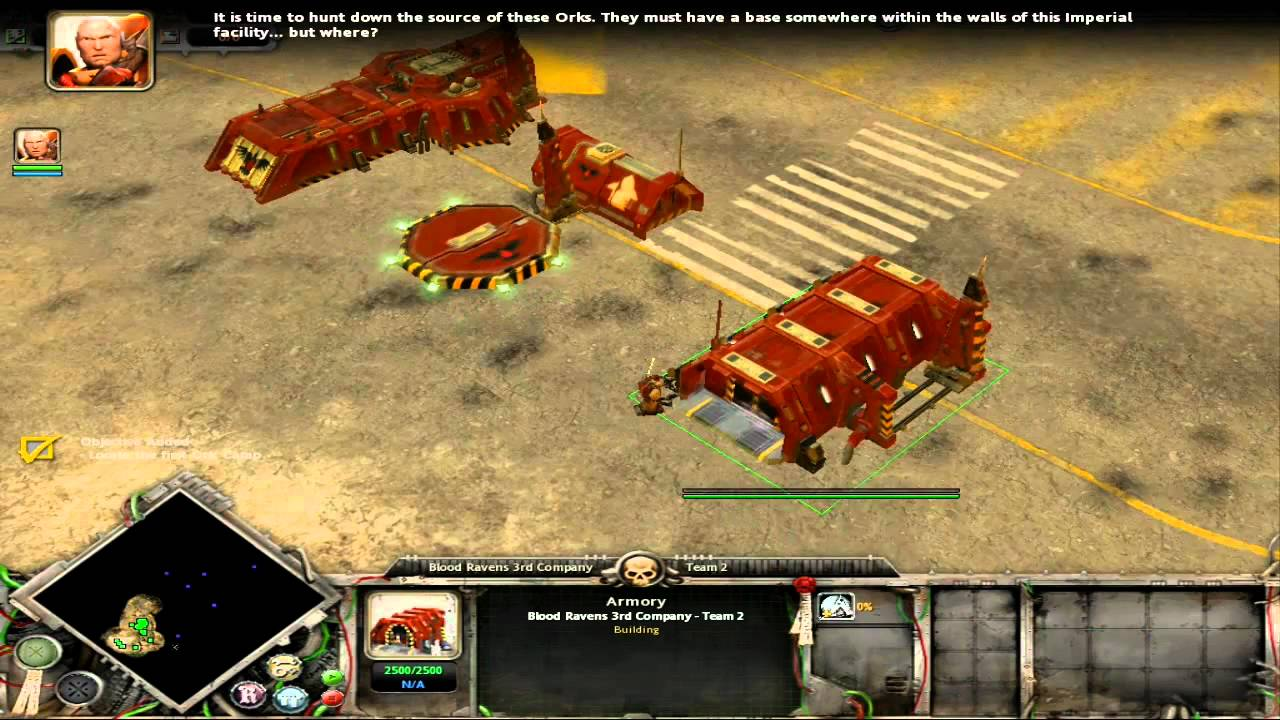
\includegraphics[width=1.0\textwidth]{images/warhammer1.jpg}
    \caption[Budowanie budynku przez dedykowaną do tego jednostkę w grze \textit{Warhammer 40,000: Dawn of War}.]{Budowanie budynku przez dedykowaną do tego jednostkę w grze \textit{Warhammer 40,000: Dawn of War}\protect\footnotemark.}
\end{figure}
\FloatBarrier
\footnotetext{Internet, \url{https://www.youtube.com/watch?v=wNtnGFoVReU}, dostęp: 19.11.2023}

\section{Mechanizm walki oraz zarządzania ekwipunkiem w Kingdom Come: Deliverance [Bogna Lew]}

Kingdom Come: Deliverance to gra z gatunku RPG osadzoną w realiach Europy Środkowej na początku XV wieku. Chociaż nie
jest to gra czasu rzeczywistego to jest to pozycja warta wymienienia ze względu na dbałość twórców o zachowanie realizmu
epoki oraz staranność wykonania mechanizmów walki oraz zarządzania ekwipunkiem. Jest ona przeznaczona dla jednego gracza,
a całość zaprezentowana jest z perspektywy pierwszoosobowej. W trakcie rozgrywki użytkownik rozwija swoją postać, bierze
udział w starciach, prowadzi rozmowy z niezależnymi postaciami i wiele więcej.

Godny uwagi jest mechanizm walki. Twórcy skupili się na jak najdokładniejszym oddaniu średniowiecznego stylu walki. W tym
celu skrupulatnie przestudiowali w jaki sposób władano mieczem w tamtych czasach, a następnie w pełni oddali to w grze.
Wykorzystali do tego tysiące animacji oraz starannie oddali fizykę pojedynków. W efekcie powstał realistyczny mechanizm
walki, który umożliwia graczowi parowanie, zadawanie ciosów oraz blokowanie.

Kolejnym elementem wartym wymienienia jest rozbudowany system zarządzania ekwipunkiem. Przeznaczony do tego panel jest
podzielony na dwie sekcje - jedna w której wyświetlona jest lista posiadanych rzeczy oraz druga przeznaczona na postać
gracza. Może on dowolnie spersonalizować swoją postać, poprzez możliwość założenia wielu elementów ubioru naraz tworząc
warstwy.  Dodatkowo, każdy przedmiot posiada swoją wagę, a postać swój maksymalny udźwig. W przypadku przekroczenia limitu
gracz zostaje ukarany poprzez spowolnienie ruchów w walce i uniemożliwieniu biegania. Jest to wzorowane na rzeczywistości,
dzięki czemu gra jeszcze lepiej oddaje realia epoki.

\section{Pasek najważniejszych informacji w interfejsie użytkownika gry Warcraft3 (Zofia Sosińska)}\label{c:pasek_war3}
Gra Warcraft III: Reign of Chaos studia Blizzard Entertainment skupia informacje o czasie gry i inwentarzu w cienkim pasku na samej górze ekranu. 
Takie graficzne przedstawienie najważniejszych danych z otoczenia gracza nazywamy interfejsem użytkownika UI (ang. \textit{user interface}). Narzędziami odzwierciedlania informacji
w czytelny i przystępny sposób mogą być takie elementy jak obrazki, teksty, czy wskaźniki. Dzięki UI możliwy jest wgląd w aktualny stan wiedzy grywalnej postaci, a tym samym lepsze
 zrozumienie otoczenia. Wymagające podkreślenia jest, że “[...] na stopień zaangażowania gracza na poziomie świata gry duży wpływ ma interfejs, którym się posługuje. Mówiąc najprościej:
  gracz, który rozpoczyna grę, zanim dozna poczucia integracji ze sterowaną przez siebie postacią, musi - używając stwierdzenia Aarsetha - spełnić oczekiwania interfejsu.”\cite{olbrzymwcieniu}

Skład elementów tej części interfjsu użytkownika gry Warcraft III jest niezmienny: pola otwierające zakładki, pora dnia oraz trzy wskaźniki zasobów. Pasek jest widoczny
podczas całej rozgrywki, niezależnie od wykonywanych czynności. W tym statycznie zakotwiczonym na górze ekranu elemencie, dynamicznie
zmieniają się jedynie ciągle aktualizowane informacje. Odpowiednio podmieniana jest tekstura pory dnia, zmieniająca się ze Słońca
na Księżyc oraz stan zasobów, zależnie od wydania, czy pozyskania.


\begin{figure}[htbp]
    \centering
    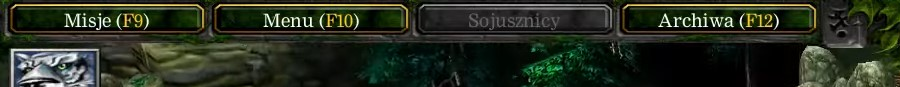
\includegraphics[width=1.0\textwidth]{images/ui/warcraft3_gorny_pasek_lewy.png}
    \caption{Lewa część paska z informacjami w grze Warcraft 3.}\label{fig:Warcraft3}
\end{figure}

\begin{figure}[htbp]
    \centering
    
\includegraphics[width=1.0\textwidth]{images/ui/warcraft3_gorny_pasek_prawy.png}
    \caption{Prawa część paska z informacjami w grze Warcraft 3.}\label{fig:Warcraft3}
\end{figure}
\section{System dialogów w grach (Bartosz Strzelecki)}\label{chap:dialogi}
Systemy dialogów w grach wideo kształtują wciągającą historię, umożliwiając graczom dokonywanie wyborów, które wpływają na relacje między postaciami, zadania i narrację gry. 
Odkrywają wiedzę, pogłębiają zaangażowanie i oferują dynamiczną rozgrywkę poprzez różnorodne podejmowanie decyzji.

W Mass Effect 3 system dialogowy jest integralną częścią rozgrywki, pozwalając graczom na prowadzenie rozmów z różnymi postaciami w trakcie gry.
System dialogów w Mass Effect 3 wykorzystuje interfejs oparty na kole dialogowym (rys. \ref{fig:wheel}), które
przedstawia graczom wiele opcji odpowiedzi podczas rozmów, zwykle podzielonych na kategorie według ich ogólnego tonu lub intencji.
Dostępne opcje często obejmują wybory, dyplomatyczne, agresywne, konfrontacyjne oraz opcje neutralne lub śledcze.
Podczas niektórych rozmów lub przerywników filmowych gracze mogą przerwać trwającą rozmowę, szybko wybierając określoną opcję dialogową.
Te opcje przerywania pozwalają graczom podjąć natychmiastowe działania lub podjąć decyzje na miejscu, często wpływając na wynik sytuacji lub relacje postaci z innymi.
Ogólnie rzecz biorąc, system dialogowy w Mass Effect 3 został zaprojektowany tak, aby zapewnić graczom bogate i wciągające doświadczenie w opowiadaniu historii,
pozwalając im kształtować narrację poprzez wybory i interakcje z olbrzymią gamą postaci. System oferuje różnorodne opcje odpowiedzi, dynamiczne rozmowy i konsekwencje,
przyczyniając się do fascynującej i rozgałęzionej narracji gry.

Alternatywnym rozwiązaniem jest to zaprezentowane w grze Fallout 3 (rys. \ref{fig:fallout}). Odróżniają je przede wszystkim możliwe odpowiedzi gracza.
W tym przypadku użytkownik wybiera z listy gotową odpowiedź, zamiast jedynie tonu jak w grze MassEffect. Pozwala to na większą kontrolę
przez gracza oraz umożliwia uniknięcie sytuacji, w której gracz spodziewał się innej odpowiedzi, wybierając daną opcję dialogową.

\begin{figure}[h]
\centering
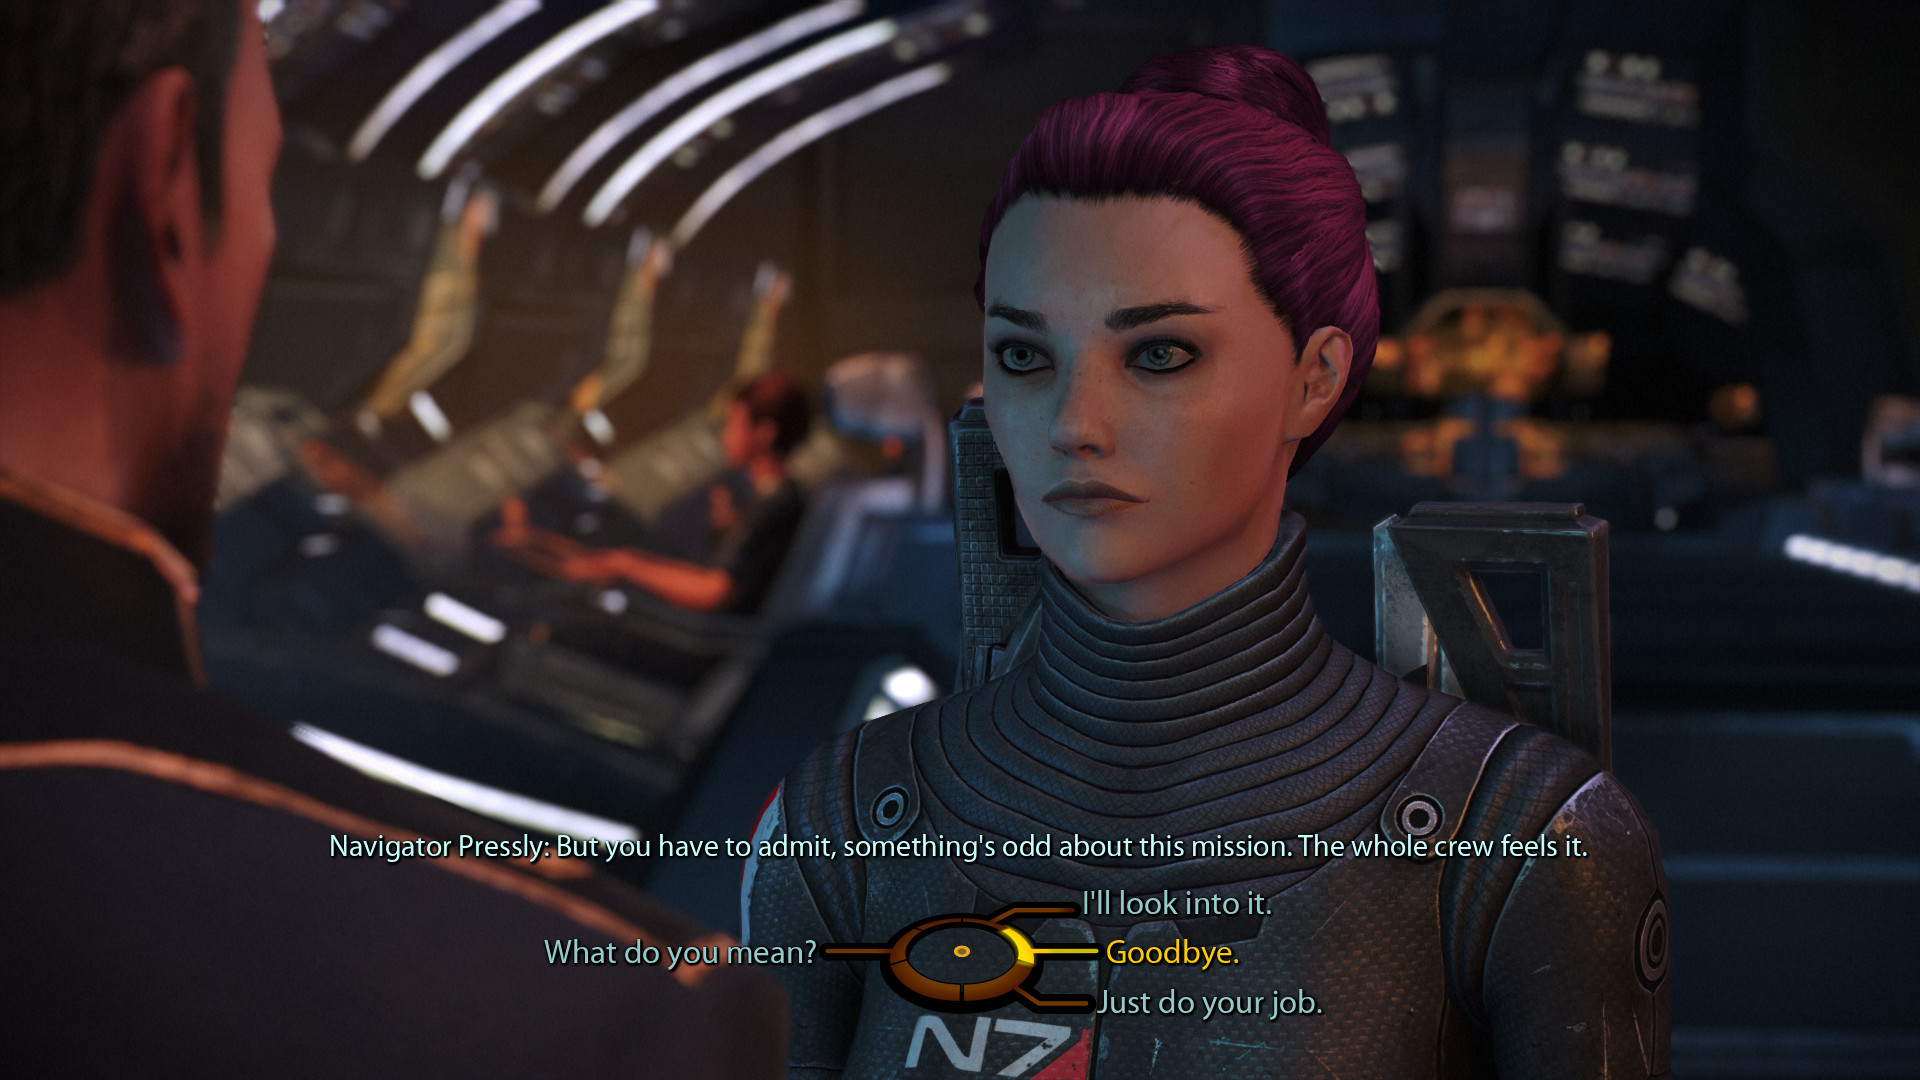
\includegraphics[width=1\textwidth]{images/me}
\caption{Przykład koła dialogowego w grze Mass Effect}
\label{fig:wheel}
\end{figure}

\begin{figure}[h]
\centering
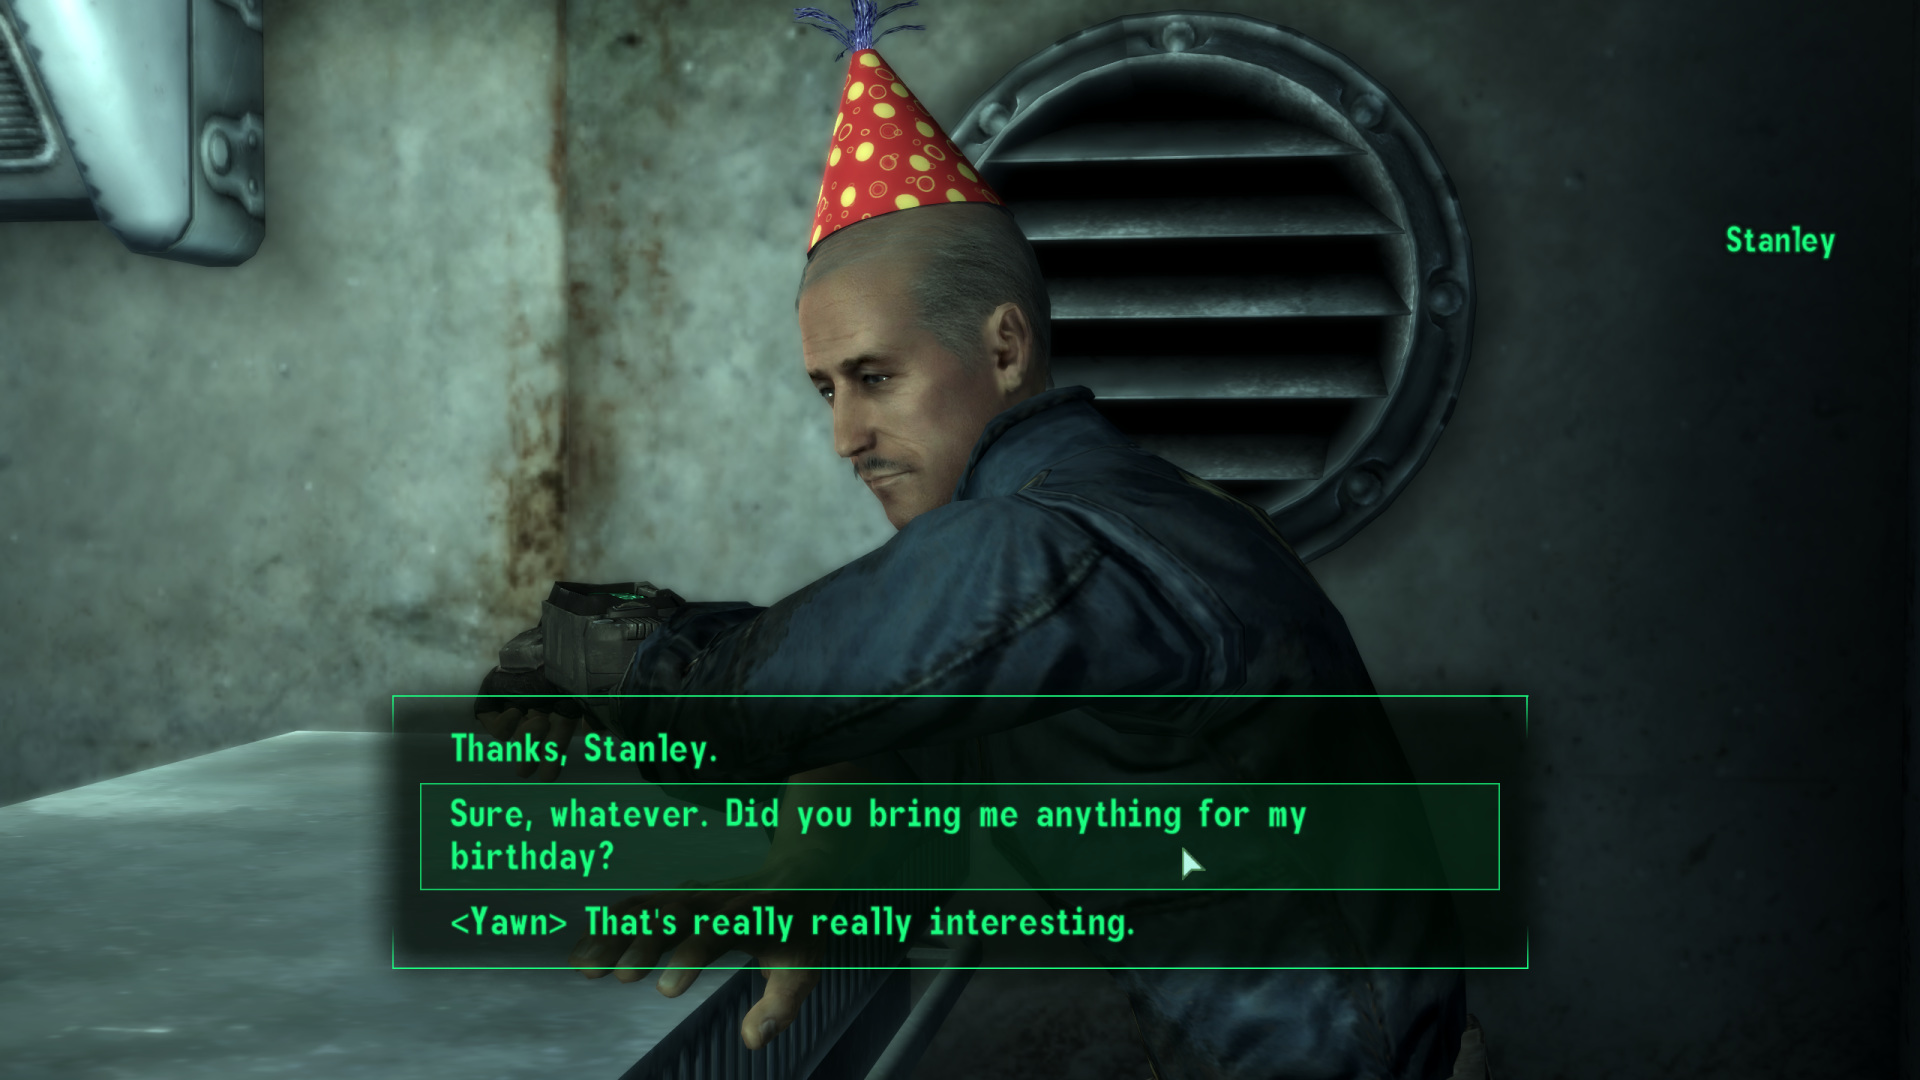
\includegraphics[width=1\textwidth]{images/fallout3}
\caption{Kadr z gry Fallout 3 przedstawiający przykładowy dialog}
\label{fig:fallout}
\end{figure}


\section{Sterowanie jednostkami w grze Mount\&Blade (Zofia Sosińska)}\label{chap:mb}

Mount\&Blade jest to gra komputerowa z gatunku cRPG (komputerowa gra fabularna, ang. computer role-playing game) z elementami strategicznymi, stworzona przez turecką firmę TaleWorlds Entertainment i wydana przez Paradox Interactive. W otwartym świecie fikcyjnej krainy Calradia, stylizowanej na czasy średniowieczne, gracz ma pełną dowolność stylu rozgrywki. W jego mocy jest zarówno zbieranie armii i dążenie do zostania królem, jak i zostanie wasalem jednego z władców. Za pomocą dialogów i walk z postaciami gracz buduje unikatową historię.
Jedną z wartych uwagi mechanik, zaimplementowaną w grze Mount\&Blade, jest sterowanie jednostkami służącymi granemu charakterowi. Gracz bezpośrednio kieruje jedynie główną postacią. Podczas walki reszcie może wydawać rozkazy. Poprzez cyfry 0-4 wybiera grupę, do której się odnosi np. łuczników. Następnie przez klawisze F1-F11 wydaje konkretny rozkaz np. odwrót. Sztuczna inteligencja postaci zajmuje się już samym wykonaniem czynności. Gracz nie martwi się, czy jednostki znajdą optymalną drogę, będą celować w przeciwników, czy z nimi walczyć.


\section{Kompasy w grach (Zofia Sosińska)}\label{chap:skrm}
Częstą funkcjonalnością gier jest możliwość eksploracji świata, w którym na gracza czekają przygody i zadania do wykonania.
Jednak przestrzeń przygotowana dla użytkownika może być na tyle duża i skomplikowana, że powstaje ryzyko 
zgubienia się. Jednym ze sposobów jakim projektanci gier wyciągają rękę do zatraconego w labiryncie użytkownika jest danie mu
kompasu. Może to być bardzo proste narzędzie, pokazujące jedynie strony świata, immitujące klasyczny przedmiot ze świata rzeczywistego.
Już taka garstka informacji potrafi uprościć graczowi odnalezienie drogi do celu. Jednak innym podejściem jest rozrzerzenie 
funkcjonalności kompasu o pokazywanie pozycji innych ważnych punktów odniesienia, celów, do których trzeba się dostać, lub 
kluczowych posatci.

The Elder Scrolls V: Skyrim (skrótowo Skyrim) jest to fabularna gra
wyprodukowana przez Bethesda Game Studios i wydana przez Bethesda Softworks. Autorzy przygotowali dla gracza duży świat,
który ten może dowolnie eksplorować. Nawigację oparli o bardzo pomocne i sprytne rozwiązanie,
jakim jest pasek przedstawiający pole widzenia gracza. Służy on między innymi jako kompas, ponieważ 
jedną z jego mechanik jest pokazanie użytkownikowi stron świata, znajdujących się w kierunku, w którym 
on patrzy. Pasek ułatwia także poruszanie się po świecie, sygnalizując położenie wrogów, kompanów i ważnych 
dla rozgrywki lokalizacji.

\begin{figure}[htbp]
	\centering
	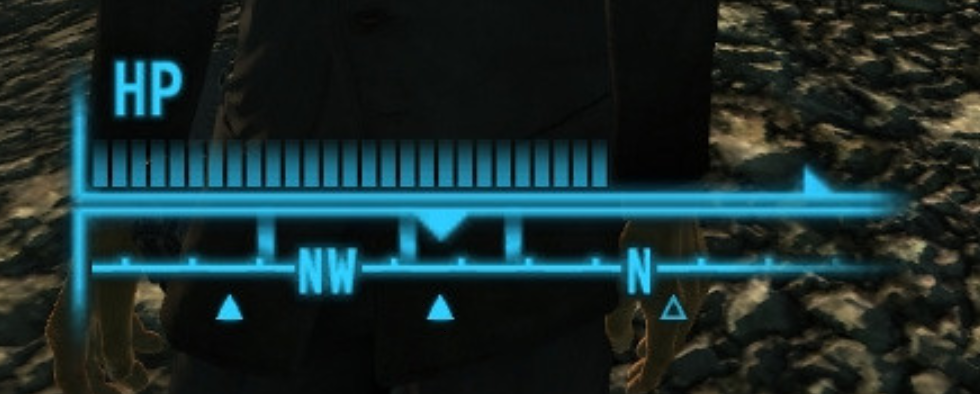
\includegraphics[width=0.9\textwidth]{images/ui/compassSkyrim.png}
	\caption{Kompas z gry Skyrim}\label{fig:Fallout}
\end{figure}


\section{Stawianie budowli (Zofia Sosińska)}\label{chap:omd}
Jedną z kluczowych mechanik gier z gatunku RTS jest budowanie budynków. Funkcjonalność pozwala graczowi 
na podejmowanie strategicznych decyzji w zależności od potrzeb i możliwości budowli. Funkcje pełnione 
przez budynek mogą być bardzo różnorodne. W niektórych przypadkach ich zadaniem jest produkcja surowców, czy leczenie
jednostek, ale są i takie, które skupiają się na wspieraniu w obliczu bitwy. Mogą to być fortyfikacje opóźniające natarcie,
bądź chociażby machiny wojenne towarzyszące ofensywie.

Orcs must die! to strategiczna gra akcji stworzona i wydana przez studio Robot Entertainment. Zadaniem gracza jest wcielenie się
w jednego z  Wojennych Magów i mordowanie nadciągających grup orków za pomocą różnorodnych broni i mechanizmów, które może postawić.
W przejrzysty sposób zostało rozwiązane samo wyświetlenie dostępnych do zbudowania pułapek. Na dole ekranu pokazują się wizerunki mechanizmów,
które może postawić oraz informacja o ich cenie. Naciskając odpowiedni numer na klawiaturze, gracz wybiera, co chce zbudować. Po zatwierdzeniu lewym przyciskiem myszki,
budynek pojawia się w zaznaczonym miejscu. Od tego momentu pułapka będzie pomocą dla głównej postaci podczas zwarcia z przeciwnikami.
Jego ograniczeniem w stawianu mechanizmów są jego fundusze, dlatego musi przemysleć, co kupić oraz gdzie najoptymalniej będzie to postaawić.

\begin{figure}[h!tbp]
    \centering
    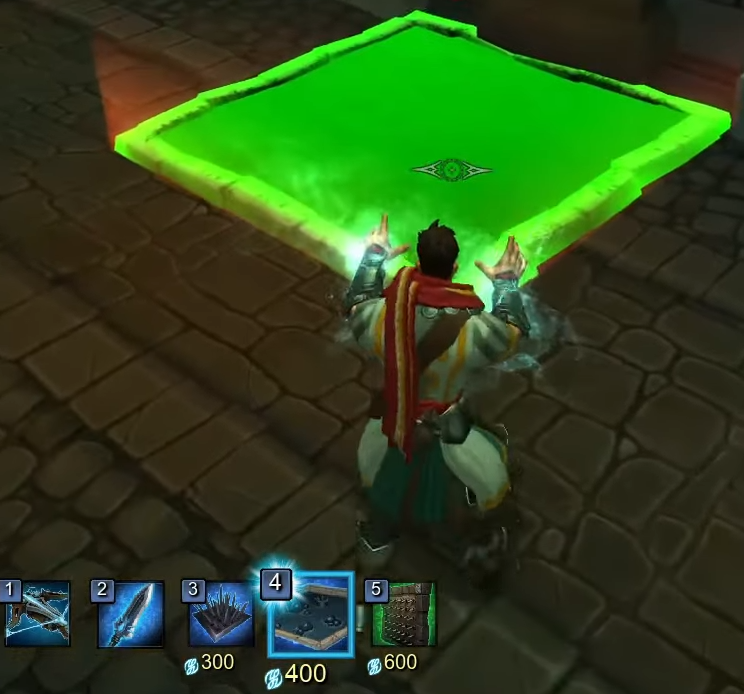
\includegraphics[width=0.9\textwidth]{images/ui/buoildingsOrcs.png}
    \caption{Wyświetlenie dostępnych pułapek w Orcs must die!}\label{fig:Orcs}
\end{figure}
\section{Przekazywanie informacji o świecie w grach (Bartosz Strzelecki)}\label{chap:dbd}
Systemy przekazywania graczowi informacji o świecie są nieocenioną pomocą w kształtowaniu dynamiki i dostarczaniu kluczowych informacji.
Jest to podstawowy element rozgrywki, pozwalający na dynamiczne podejmowanie decyzji oraz na koordynację działań w grach wieloosobowych.

Gra \textit{Dead by Daylight}\footnote{\url{https://deadbydaylight.com}} jest asymetryczną grą wieloosobową, w której gracze wcielają się w rolę postaci "ocalałych" starających się uciec
z mapy albo w rolę "zabójcy", którego celem jest niedopuszczenie do tego. Jednym z udostępnianych przez tę grę mechanizmów jest mechanika widzenia przez przeszkody, która stanowi istotny element rozgrywki, zapewniający
dodatkową warstwę strategii. Polega na wyświetlaniu reprezentacji odległych celów, przedmiotów i przeciwników
zakrytych przez przeszkody. Ta zdolność odgrywa kluczową rolę dla obu stron konfliktu.

W przypadku "ocalałych", ta mechanika jest dostępna dzięki atutom i przedmiotom. Mechanika ujawnia lokalizację celów oraz
innych "ocalałych" pozwalając na koordynację i opracowanie strategii wspólnych działań.

\begin{figure}[h]
\centering
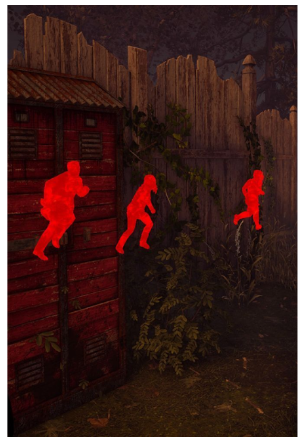
\includegraphics[width=0.4\textwidth]{images/dbd}
\caption{Przykładowy efekt aury w grze \textit{Dead by Daylight}.}
\end{figure}

I odwrotnie, zdolność "zabójcy" do widzenia aury jest kluczowa dla jego mechaniki rozgrywki.
Aury umożliwiają im śledzenie "ocalałych", zwłaszcza gdy korzystają z ich unikalnych mocy lub specyficznych atutów.
Mechanika ta zwiększa napięcie, ponieważ "ocalali" muszą zachować czujność i strategiczne podejście,
aby uniknąć pola widzenia "zabójcy" lub zakłócić ich zdolność czytania aury, aby uciec i osiągnąć cele.

% \begin{figure}[h]
% \centering
% 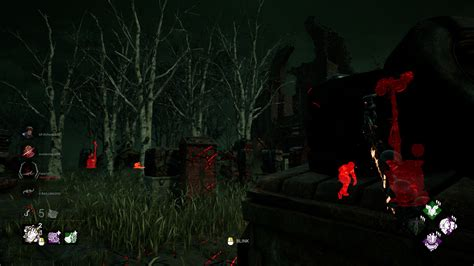
\includegraphics[width=0.6\textwidth]{images/aura}
% \caption{Przykładowe elementy widzenia przez horyzont w grze \textit{Dead by Daylight}.}
% \end{figure}

Ogólnie rzecz biorąc, mechanika aury w \textit{Dead by Daylight} służy jako podstawowy element rozgrywki,
który równoważy wymianę informacji między "ocalałymi" a "zabójcami", znacząco przyczyniając się do atmosfery napięcia i strategii w grze.


\section{Modele celowania w grach (Bartosz Strzelecki)}\label{s:cel}
Celowanie w grach taktycznych jest podstawowym elementem programu, który ma
olbrzymi wpływ na przebieg rozgrywki. Ten mechanizm jest przede wszystkim wykorzystywany
do wzbogacenia gry o kolejną warstwę decyzji taktycznych i zarządzania podejmowanym ryzykiem.
Gracz, przed oddaniem strzału, podejmuje decyzję czy warto zaryzykować podjęcie strzału o niskiej szansie
na trafienie, czy lepiej wykonać niezawodny atak, prawdopodobnie wystawiając się na ataki przeciwników.

W \textit{Phoenix Point}\footnote{\url{https://phoenixpoint.info}} modelowanie celności to wieloaspektowy system, który w zawiły sposób definiuje wynik interakcji bojowych.
Gra wykorzystuje dynamiczny system celowania, który uwzględnia różne elementy, takie jak postawa żołnierza, biegłość w posługiwaniu się bronią, zasięg, 
osłona i warunki środowiskowe, aby określić precyzję strzału. Każdy z tych elementów odgrywa znaczącą rolę w ogólnym obliczeniu trafienia w cel.

W przeciwieństwie do podobnej gry \textit{XCOM}\footnote{\url{https://www.xcom.com}}, gdzie celność jest zamodelowana za pomocą prostej szansy na trafienie, w grze \textit{Phoenix Point}
trajektoria każdego pocisku obliczana jest osobno. Podczas celowania widoczne są dwa okręgi: wewnętrzny, który reprezentuje miejsce,
w którym znajdzie się 50\% pocisków oraz zewnętrzny, który reprezentuje maksymalny rozrzut broni. W tym przypadku im celniejsza broń tym
okręgi będą mniejsze.

\begin{figure}[h]
\centering
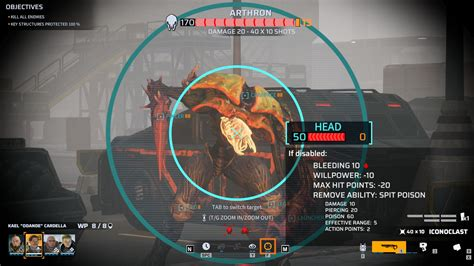
\includegraphics[width=1\textwidth]{images/point}
\caption[System celowania występujący w grze \textit{Phoenix Point}.]{System celowania występujący w grze \textit{Phoenix Point}\protect\footnotemark.}
\label{fig:acc}
\end{figure}
\footnotetext{Internet, \url{https://www.pcgamesn.com/wp-content/uploads/2019/12/phoenix-point-aim.jpg}, dostęp: 16.08.2023}
\FloatBarrier
Ostatecznie system zaimplementowany w grze \textit{Phoenix Point} okazuje się dużo bardziej realistyczny i pozwala na utrzymywanie ciągłej niepewności
co do celności strzału, umożliwiając w ten sposób na strategiczne wyzwania, leżących u podstaw gier tego typu. 

\section{Fabuła w grach (Bogna Lew)}\label{s:fabula}
W przypadku wielu gier, niezależnie od gatunku, kluczową rolę odgrywa fabuła. To ona sprawia, że gra przestaje być
jedynie programem wykonującym polecenia, a staje się opowieścią będącą formą rozrywki. Ważnym aspektem fabuły jest jej
narracja, która definiuje kolejność występowania konkretnych elementów. W odróżnieniu od narracji budującej
fabułę książki, czy filmu, narracja w grach komputerowych umożliwia graczowi wpływanie na nią. "Dobrze nakreślona
narracja wykorzystuje wybory fabularne z wielkim uwzględnieniem ogólnego celu pracy. Może obejmować ujawnienie pewnych
informacji z przeszłości, aby zwiększyć poczucie niepewności, lub wczesne informacje podstawowe, aby wzmocnić motywację
postaci" \cite{level_design}.

W grach komputerowych w skład fabuły wchodzą cel główny oraz zadania poboczne. Cel główny stanowi podstawę gry, dając
graczowi poczucie dążenia do czegoś i jest ogólnym zamysłem całej rozgrywki. Zadania poboczne natomiast są krótkimi
misjami będącymi urozmaiceniem rozgrywki. "W odniesieniu do gier komputerowych można więc mówić o podwójnym motywowaniu
ich użytkowników, które dokonuje się na dwóch narracyjnych poziomach: jedna z motywacji wyznacza cel całej
rozgrywce, druga natomiast jest ulokowana w przestrzeni pojedynczej misji i kończy wraz z jej zakończeniem" \cite{olbrzymwcieniu}.

Innym elementem budującym fabułę są przerywniki filmowe, które wprowadzają nowe informacje i wydarzenia. "Wiele gier z
wyrafinowaną fabułą wykorzystuje tę technikę do umiejscowienia działań gracza w fikcyjnym świecie, który dzięki temu
może zostać opisany z dużą kontrolą po stronie autora." \cite{understanding_games}. Stanowią one ciekawe urozmaicenie w rozgrywce i
pozwalają na przekazanie graczowi więcej informacji.

W przypadku gier strategii czasu rzeczywistego fabuła występuje w trybie kampanii tych gier. Każda z pojedynczych bitew
stanowi fragment większej historii występującej w kampanii. Typowo w grach typu RTS występuje fabuła liniowa.
Przykładowo w grze \textit{Warhammer 40,000: Dawn of War} ogólnym zamysłem kampanii jest obrona planety przed najazdem wroga.
Zrealizowana jest za pomocną jedenastu misji, w których gracz ma do realizacji pewne cele, takie jak zajęcie określonej
liczby punktów kontrolnych, czy zniszczenie bazy przeciwnika. Pomiędzy misjami występują przerywniki filmowe, które
to odkrywają przed graczem kolejne elementy historii.

W tym miejscu warto wspomnieć System Nemesis występujący w grze \textit{Middle-earth: Shadow of Mordor} i rozwinięty w
\textit{Middle-earth: Shadow of War}\footnote{\url{https://www.shadowofwar.com/}}. Chociaż wymienione gry nie są z gatunku strategii czasu rzeczywistego to ta mechanika jest
interesującym przykładem kształtowania fabuły w grze. System Nemesis jest mechanizmem generowania przeciwników, który nadaje
każdemu z nich ich unikalny charakter oraz wygląd. W ciągu gry system Nemesis dynamicznie wpływa na postacie, rozwijając
je i odpowiednio zmieniając ich wygląd. Efektem tego jest płynnie zmieniająca się fabuła, która dla każdego gracza
będzie inna.

Do podstawowych elementów tej mechaniki należy rozbudowany system relacji pomiędzy postaciami w grze, w tym postaci
gracza. Dodatkowo buduje ona hierarchię wśród Orków, dynamicznie ją aktualizując w trakcie gry w zależności od śmierci
poszczególnych bohaterów oraz postaci gracza.

\begin{figure}[h!]
    \centering
    
\includegraphics[width=0.9\textwidth]{images/system_nemesis.jpg}
    \caption[Przykładowa postać przeciwnika utworzona przez system Nemesis.]{Przykładowa postać przeciwnika utworzona przez system Nemesis.\protect\footnotemark}
\end{figure}
\footnotetext{Internet, \url{https://www.youtube.com/watch?v=liMe8E4ODIs}, dostęp: 20.11.2023}

System Nemesis jest interesującą mechaniką budującą fabułę w grze. Pozwala na zbudowanie unikatowych przeciwników,
którzy mają bezpośredni wpływ na rozgrywkę i kształtowanie jej przebiegu.


\section{System dialogów w grach (Bartosz Strzelecki)}\label{chap:dialogi}
Systemy dialogów w grach wideo kształtują wciągającą historię, umożliwiając graczom dokonywanie wyborów, które wpływają na relacje między postaciami, zadania i narrację gry. 
Odkrywają wiedzę, pogłębiają zaangażowanie i oferują dynamiczną rozgrywkę poprzez różnorodne podejmowanie decyzji.

W Mass Effect 3 system dialogowy jest integralną częścią rozgrywki, pozwalając graczom na prowadzenie rozmów z różnymi postaciami w trakcie gry.
System dialogów w Mass Effect 3 wykorzystuje interfejs oparty na kole dialogowym (rys. \ref{fig:wheel}), które
przedstawia graczom wiele opcji odpowiedzi podczas rozmów, zwykle podzielonych na kategorie według ich ogólnego tonu lub intencji.
Dostępne opcje często obejmują wybory, dyplomatyczne, agresywne, konfrontacyjne oraz opcje neutralne lub śledcze.
Podczas niektórych rozmów lub przerywników filmowych gracze mogą przerwać trwającą rozmowę, szybko wybierając określoną opcję dialogową.
Te opcje przerywania pozwalają graczom podjąć natychmiastowe działania lub podjąć decyzje na miejscu, często wpływając na wynik sytuacji lub relacje postaci z innymi.
Ogólnie rzecz biorąc, system dialogowy w Mass Effect 3 został zaprojektowany tak, aby zapewnić graczom bogate i wciągające doświadczenie w opowiadaniu historii,
pozwalając im kształtować narrację poprzez wybory i interakcje z olbrzymią gamą postaci. System oferuje różnorodne opcje odpowiedzi, dynamiczne rozmowy i konsekwencje,
przyczyniając się do fascynującej i rozgałęzionej narracji gry.

Alternatywnym rozwiązaniem jest to zaprezentowane w grze Fallout 3 (rys. \ref{fig:fallout}). Odróżniają je przede wszystkim możliwe odpowiedzi gracza.
W tym przypadku użytkownik wybiera z listy gotową odpowiedź, zamiast jedynie tonu jak w grze MassEffect. Pozwala to na większą kontrolę
przez gracza oraz umożliwia uniknięcie sytuacji, w której gracz spodziewał się innej odpowiedzi, wybierając daną opcję dialogową.

\begin{figure}[h]
\centering
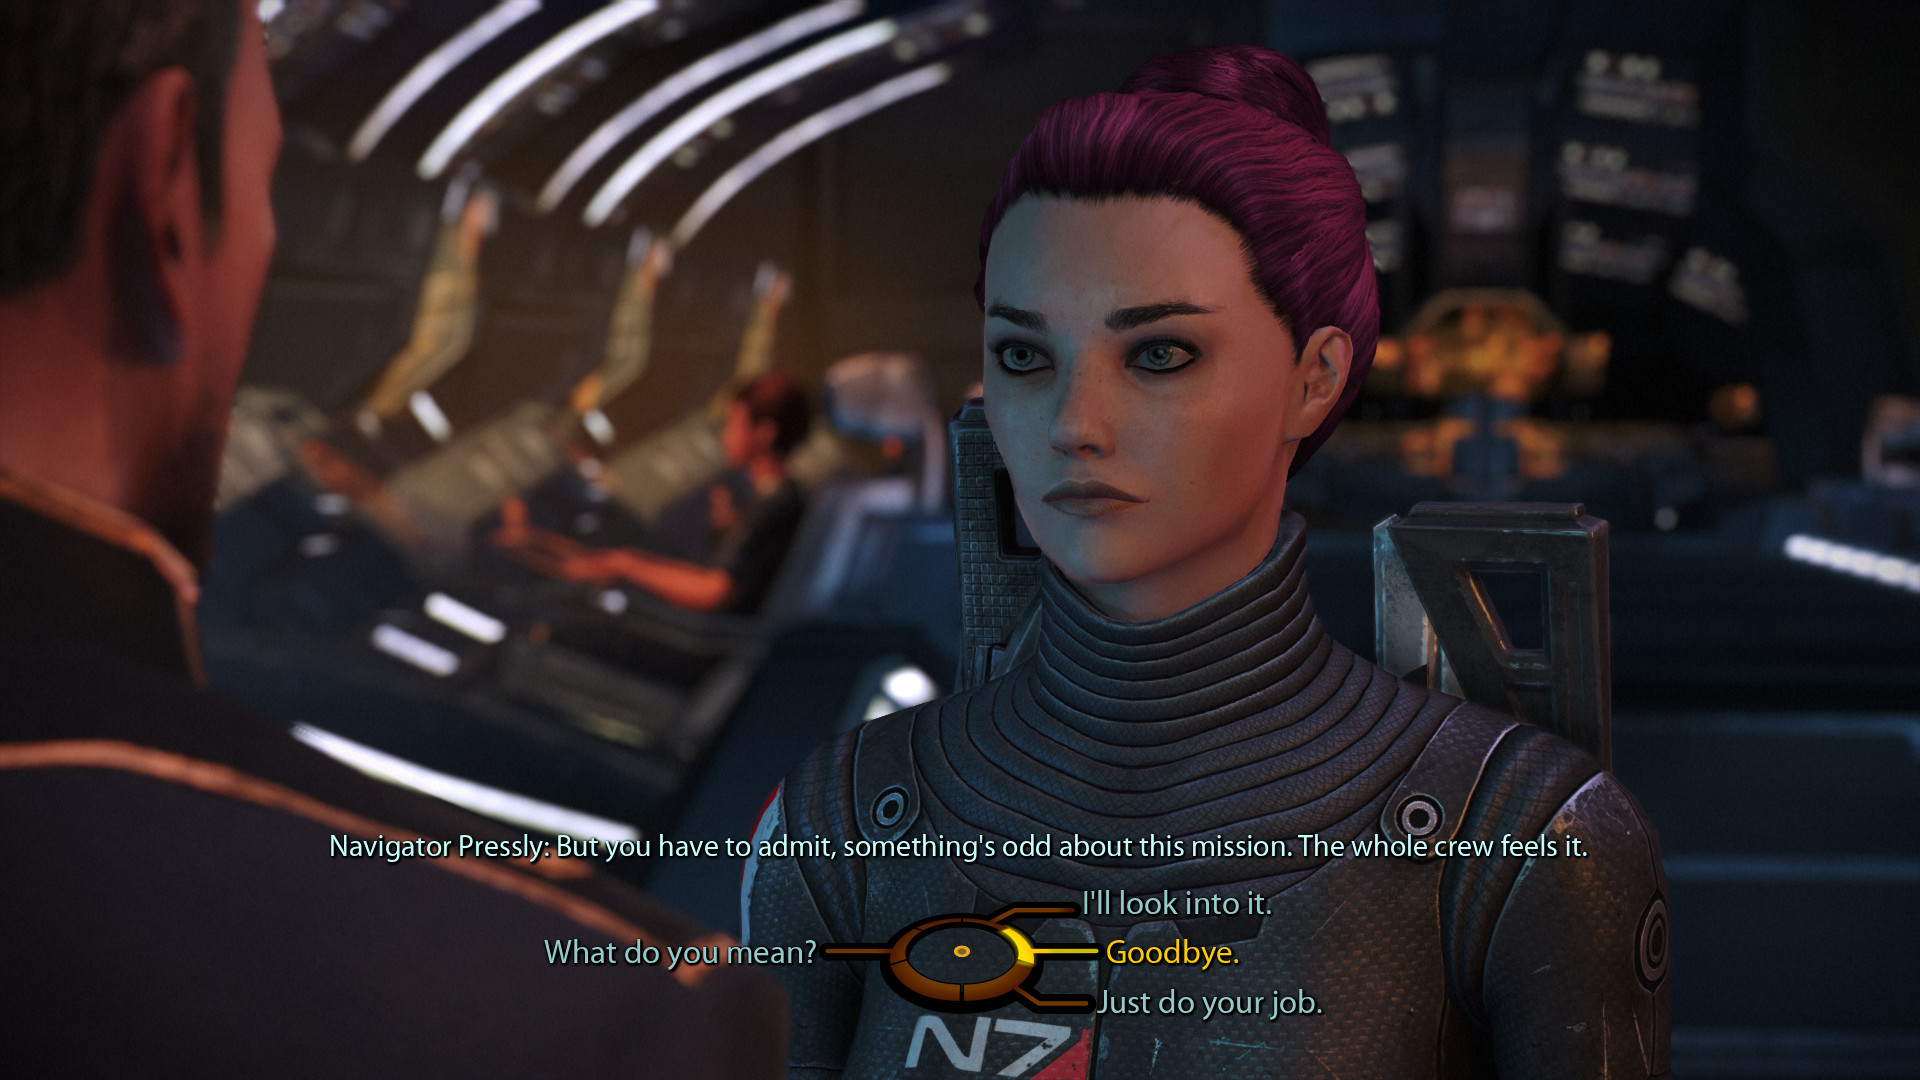
\includegraphics[width=1\textwidth]{images/me}
\caption{Przykład koła dialogowego w grze Mass Effect}
\label{fig:wheel}
\end{figure}

\begin{figure}[h]
\centering
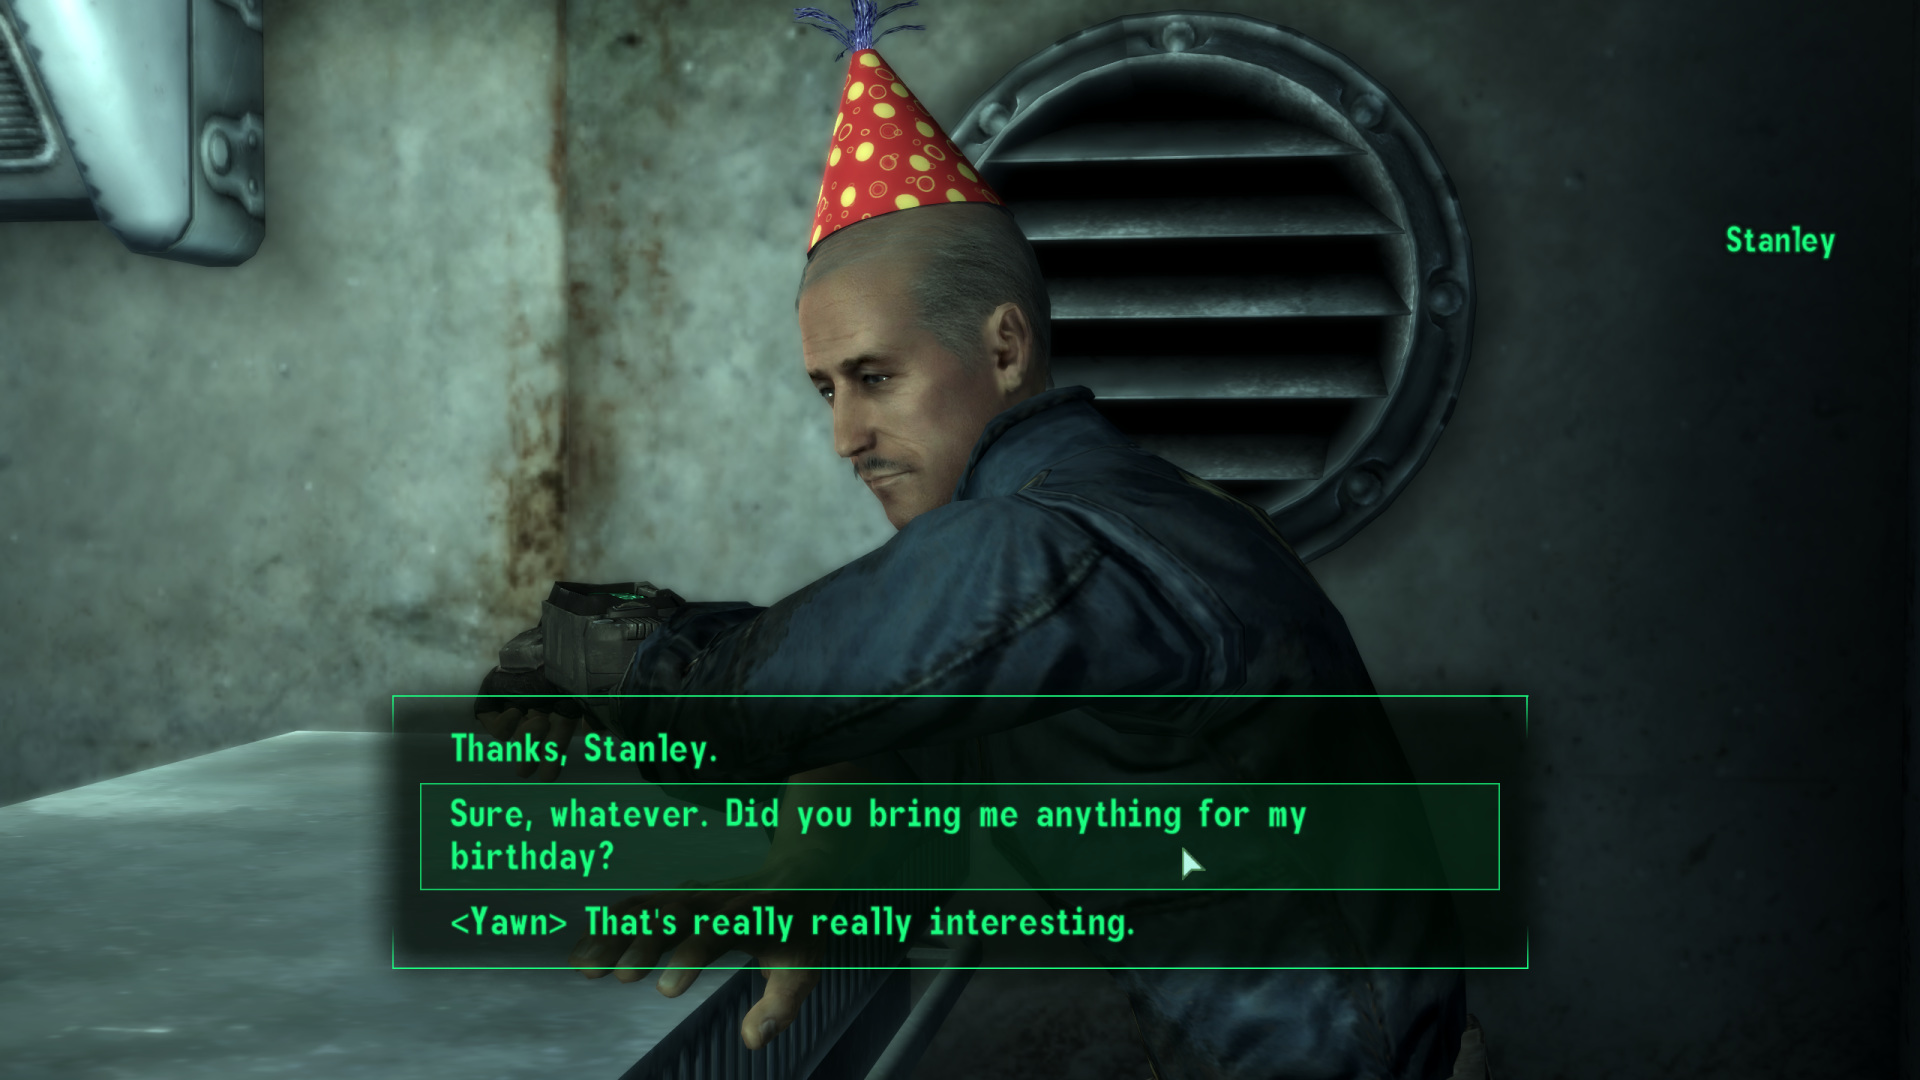
\includegraphics[width=1\textwidth]{images/fallout3}
\caption{Kadr z gry Fallout 3 przedstawiający przykładowy dialog}
\label{fig:fallout}
\end{figure}


\section{Model sztucznej inteligencji przeciwników w grach RTS (Bartosz Strzelecki)}
W sferze gier RTS sztuczna inteligencja (ang. artificial intelligence, AI) odgrywa kluczową rolę, wspierając doświadczenia z rozgrywki.
W tym przypadku termin odnosi się do zbioru algorytmów i systemów zaprojektowanych w celu symulacji
zachowań podobnych do tych gracza. Między innymi umiejętność podejmowania decyzji i rozwiązywania problemów.

Sztuczna inteligencja przeciwników w grach takich jak Warcraft III lub StarCraft II, przede wszystkim w trybie kampanii,
jest odpowiedzialna za kontrolowanie wrogich jednostek w celu zaoferowania graczowi wyzwania. Głównym zadaniem AI jest zasymulowanie
strategicznych decyzji i wydajne zarządzanie zasobami.
AI podejmuje decyzję na podstawie predefiniowanych zasad i algorytmów. Analizuje sytuację, w której się znajduje, biorąc pod uwagę
siłę swojej własnej armii, siłę armii gracza oraz specjalne zdolności jednostek i środowisko, w którym toczy się gra.
Ta analiza pozwala komputerowi na podejmowanie strategicznych decyzji jak na przykład, kiedy atakować, bronić się, eksplorować oraz rozszerzać swoje terytorium.
W tych grach sztuczna inteligencja może przybrać jeden z kilku wariantów wynikających z poziomu trudności. Wyższe poziomy
dają przeciwnikowi przewagę taką, jak wydajniejsze zbieranie zasobów lub szybsza produkcja jednostek.

W grze Warcraft III w trybie kampanii zachowanie przeciwników jest zaprojektowane z myślą o zanurzeniu gracza w fabularnej opowieści, jednocześnie
prezentując wciągające wyzwania związane z rozgrywką. Akcje wykonywane przez sztuczną inteligencję są dostosowane do celów danej misji, co pozwala
na dopasowanie do obowiązującej narracji.
Początkowo przeciwnik konstruuje i rozbudowuje swoją bazę, w celu zgromadzenia odpowiedniej liczby zasobów, szkolenia jednostek i prowadzenia badań.
AI strategicznie rozmieszcza budynki i struktury obronne, aby ochronić swoją fortecę przed najazdami gracza. 
Misje kampanii często też zawierają oskryptowane wydarzenia lub walki, które dodają głębi rozgrywce. Podczas tych starć wroga sztuczna inteligencja
może zachowywać się w specjalny sposób, kontrolując potężne jednostki, do których gracz normalnie nie ma dostępu lub inicjując działania, które popychają
narrację do przodu. Te wyreżyserowane wydarzenia tworzą niezapomniane chwile i jeszcze bardziej wciągają gracza w fabułę kampanii.
Zachowanie wroga w kampanii jest zróżnicowane i obejmuje różnorodne cele misji i scenariusze. Gracze mogą napotkać wrogów, którzy preferują agresywne ataki,
inni skupiają się na strategiach obronnych lub specjalizują się w taktyce hit and run. Sztuczna inteligencja dostosowuje proces podejmowania decyzji do
konkretnych wymagań misji, często wykorzystując ukształtowanie terenu, synergię jednostek i scenariusze wydarzeń, aby rzucić wyzwanie umiejętnościom gracza.
Ogólnie rzecz biorąc, zachowanie wrogów w kampanii Warcraft III ma na celu zapewnienie dynamicznego i wciągającego doświadczenia. Gracze muszą 
wykorzystywać myślenie strategiczne, zarządzanie zasobami i efektywny skład jednostek, aby przezwyciężyć różnorodne strategie stosowane przez wrogą sztuczną inteligencję.

\section{Mechanizm budowania oraz zarządzanie zasobami w grach RTS (Bogna Lew)}\label{s:budowanie}
Jednym z typowych elementów gier strategii czasu rzeczywistego  jest tworzenie baz i budowanie fortyfikacji. Mechanizm
ten stanowi urozmaicenie rozgrywki i wprowadza dodatkowe aspekty możliwe do uwzględnienia w planowaniu strategii. Dla
wielu gier RTS jest wręcz nieodłącznym elementem, który umożliwia graczowi tworzenie i rozwój nowych jednostek,
produkcję zasobów, umacnianie swojej pozycji oraz zwiększanie swojej potęgi.

Mechanizm ten wiąże się z szeregiem ograniczeń, które mają kluczowy wpływ na rozgrywkę. Należą do nich między innymi
ograniczenia związane z ukształtowaniem terenu oraz obecnością innych elementów scenerii. Każde z tych ograniczeń ma
swoje źródło w prawdziwym świecie i mechanizm budowania musi je uwzględniać.

Z tą mechaniką związany jest system zasobów, który jest popularnym aspektem gier z tego gatunku. Wiele gier strategii
czasu rzeczywistego umożliwia graczowi budowanie własnej ekonomii. Uzyskane przez niego zasoby często mogą zostać
wykorzystane przez mechanizm budowania jako koszta budowy obiektów.

Przykładem gry strategii czasu rzeczywistego implementującej tę mechanikę jest \textit{Warhammer 40,000: Dawn of War}\footnote{\url{https://www.dawnofwar.com/}}. Jest to
gra, której realia są osadzone w uniwersum gry bitewnej \textit{Warhammer 40,000}. Udostępnia ona tryb jednoosobowy oraz
wieloosobowy dla maksymalnie sześciu graczy. W pierwszym wariancie gracz wciela się w postać dowódcy
armii Space Marines z Blood Ravens i ma za zadanie zapobiec inwazji Orków. Gra \textit{Warhammer 40,000: Dawn of War} bardzo szybko
zyskała na popularności i oferowała wszystko, co było potrzebne dla tego gatunku. Z tego powodu warto się jej przyjrzeć,
pomimo faktu, że jej realia znacząco odbiegających od tych, w których zostanie osadzona tworzona przez nas gra.

\textit{Warhammer 40,000: Dawn of War} wyróżnia model pozyskiwania surowców. W grze dostępne są dwa rodzaje: Energia, która jest
generowana przez dedykowane do tego budowle oraz Rekwizycja, której szybkość wytwarzania jest uzależniona od kontrolowanych
przez gracza punktów strategicznych. Taka mechanika znacznie lepiej wpasowuje się w realia gry oraz wymusza na użytkowniku
przyjęcie agresywniejszej strategii.

Dodatkowo \textit{Warhammer 40,000: Dawn of War} posiada typowy dla gier RTS mechanizm tworzenia budowli. Gracz ma
do dyspozycji jednostki, którym może zlecić budowę wybranego przez siebie obiektu po poniesieniu kosztów jego utworzenia.
Zanim będzie możliwe rozpoczęcie budowania użytkownik musi wybrać miejsce, w którym budynek powstanie, co robi, przesuwając
jego podgląd po mapie. W tym czasie gra dokonuje walidacji miejsca i informuje gracza czy wybrany obszar jest poprawny,
odpowiednio podświetlając widok budynku. Wybudowanie obiektu nie jest natychmiastowe, co sprawia, że gra lepiej oddaje
realia, w których jest osadzona.

\begin{figure}[h!]
    \centering
    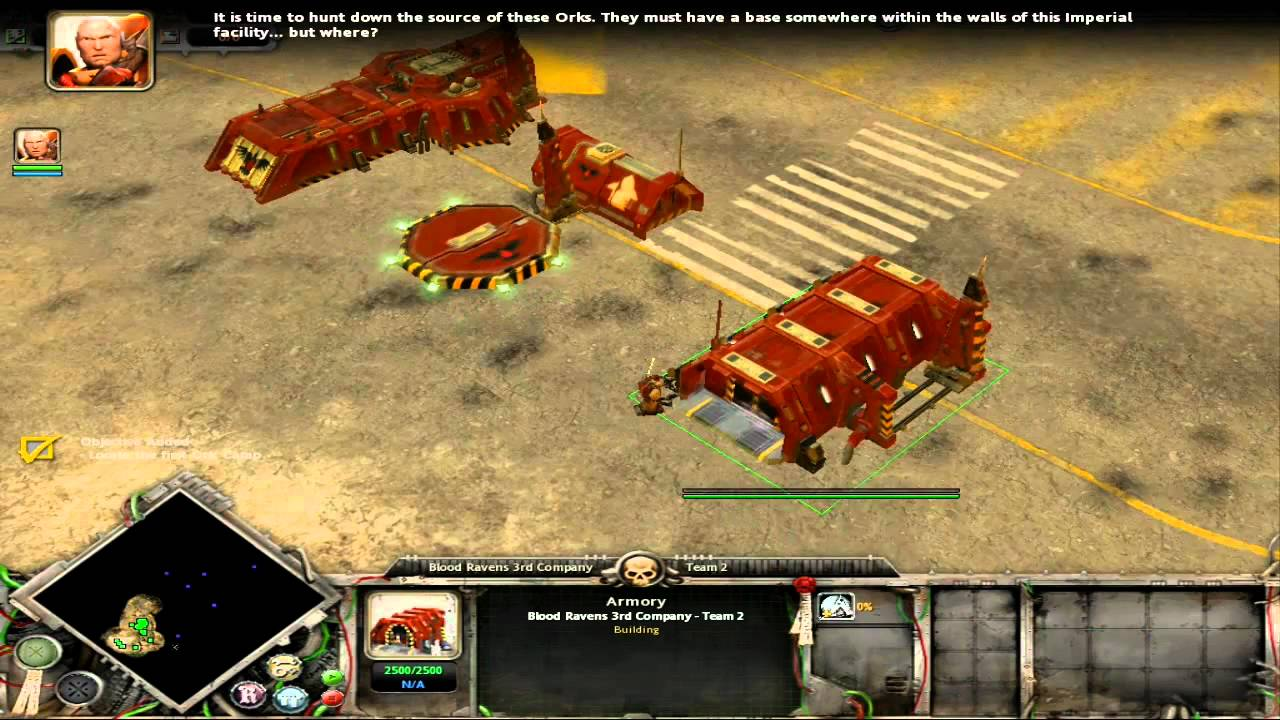
\includegraphics[width=1.0\textwidth]{images/warhammer1.jpg}
    \caption[Budowanie budynku przez dedykowaną do tego jednostkę w grze \textit{Warhammer 40,000: Dawn of War}.]{Budowanie budynku przez dedykowaną do tego jednostkę w grze \textit{Warhammer 40,000: Dawn of War}\protect\footnotemark.}
\end{figure}
\FloatBarrier
\footnotetext{Internet, \url{https://www.youtube.com/watch?v=wNtnGFoVReU}, dostęp: 19.11.2023}

\section{Mechanizm walki oraz zarządzania ekwipunkiem w Kingdom Come: Deliverance [Bogna Lew]}

Kingdom Come: Deliverance to gra z gatunku RPG osadzoną w realiach Europy Środkowej na początku XV wieku. Chociaż nie
jest to gra czasu rzeczywistego to jest to pozycja warta wymienienia ze względu na dbałość twórców o zachowanie realizmu
epoki oraz staranność wykonania mechanizmów walki oraz zarządzania ekwipunkiem. Jest ona przeznaczona dla jednego gracza,
a całość zaprezentowana jest z perspektywy pierwszoosobowej. W trakcie rozgrywki użytkownik rozwija swoją postać, bierze
udział w starciach, prowadzi rozmowy z niezależnymi postaciami i wiele więcej.

Godny uwagi jest mechanizm walki. Twórcy skupili się na jak najdokładniejszym oddaniu średniowiecznego stylu walki. W tym
celu skrupulatnie przestudiowali w jaki sposób władano mieczem w tamtych czasach, a następnie w pełni oddali to w grze.
Wykorzystali do tego tysiące animacji oraz starannie oddali fizykę pojedynków. W efekcie powstał realistyczny mechanizm
walki, który umożliwia graczowi parowanie, zadawanie ciosów oraz blokowanie.

Kolejnym elementem wartym wymienienia jest rozbudowany system zarządzania ekwipunkiem. Przeznaczony do tego panel jest
podzielony na dwie sekcje - jedna w której wyświetlona jest lista posiadanych rzeczy oraz druga przeznaczona na postać
gracza. Może on dowolnie spersonalizować swoją postać, poprzez możliwość założenia wielu elementów ubioru naraz tworząc
warstwy.  Dodatkowo, każdy przedmiot posiada swoją wagę, a postać swój maksymalny udźwig. W przypadku przekroczenia limitu
gracz zostaje ukarany poprzez spowolnienie ruchów w walce i uniemożliwieniu biegania. Jest to wzorowane na rzeczywistości,
dzięki czemu gra jeszcze lepiej oddaje realia epoki.

\section{Pasek najważniejszych informacji w interfejsie użytkownika gry Warcraft3 (Zofia Sosińska)}\label{c:pasek_war3}
Gra Warcraft III: Reign of Chaos studia Blizzard Entertainment skupia informacje o czasie gry i inwentarzu w cienkim pasku na samej górze ekranu. 
Takie graficzne przedstawienie najważniejszych danych z otoczenia gracza nazywamy interfejsem użytkownika UI (ang. \textit{user interface}). Narzędziami odzwierciedlania informacji
w czytelny i przystępny sposób mogą być takie elementy jak obrazki, teksty, czy wskaźniki. Dzięki UI możliwy jest wgląd w aktualny stan wiedzy grywalnej postaci, a tym samym lepsze
 zrozumienie otoczenia. Wymagające podkreślenia jest, że “[...] na stopień zaangażowania gracza na poziomie świata gry duży wpływ ma interfejs, którym się posługuje. Mówiąc najprościej:
  gracz, który rozpoczyna grę, zanim dozna poczucia integracji ze sterowaną przez siebie postacią, musi - używając stwierdzenia Aarsetha - spełnić oczekiwania interfejsu.”\cite{olbrzymwcieniu}

Skład elementów tej części interfjsu użytkownika gry Warcraft III jest niezmienny: pola otwierające zakładki, pora dnia oraz trzy wskaźniki zasobów. Pasek jest widoczny
podczas całej rozgrywki, niezależnie od wykonywanych czynności. W tym statycznie zakotwiczonym na górze ekranu elemencie, dynamicznie
zmieniają się jedynie ciągle aktualizowane informacje. Odpowiednio podmieniana jest tekstura pory dnia, zmieniająca się ze Słońca
na Księżyc oraz stan zasobów, zależnie od wydania, czy pozyskania.


\begin{figure}[htbp]
    \centering
    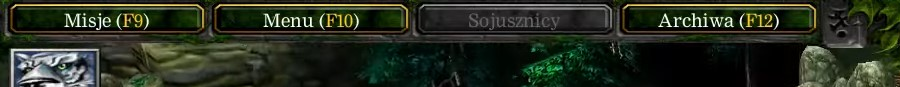
\includegraphics[width=1.0\textwidth]{images/ui/warcraft3_gorny_pasek_lewy.png}
    \caption{Lewa część paska z informacjami w grze Warcraft 3.}\label{fig:Warcraft3}
\end{figure}

\begin{figure}[htbp]
    \centering
    
\includegraphics[width=1.0\textwidth]{images/ui/warcraft3_gorny_pasek_prawy.png}
    \caption{Prawa część paska z informacjami w grze Warcraft 3.}\label{fig:Warcraft3}
\end{figure}
\section{Sterowanie jednostkami w grze Mount\&Blade (Zofia Sosińska)}\label{chap:mb}

Mount\&Blade jest to gra komputerowa z gatunku cRPG (komputerowa gra fabularna, ang. computer role-playing game) z elementami strategicznymi, stworzona przez turecką firmę TaleWorlds Entertainment i wydana przez Paradox Interactive. W otwartym świecie fikcyjnej krainy Calradia, stylizowanej na czasy średniowieczne, gracz ma pełną dowolność stylu rozgrywki. W jego mocy jest zarówno zbieranie armii i dążenie do zostania królem, jak i zostanie wasalem jednego z władców. Za pomocą dialogów i walk z postaciami gracz buduje unikatową historię.
Jedną z wartych uwagi mechanik, zaimplementowaną w grze Mount\&Blade, jest sterowanie jednostkami służącymi granemu charakterowi. Gracz bezpośrednio kieruje jedynie główną postacią. Podczas walki reszcie może wydawać rozkazy. Poprzez cyfry 0-4 wybiera grupę, do której się odnosi np. łuczników. Następnie przez klawisze F1-F11 wydaje konkretny rozkaz np. odwrót. Sztuczna inteligencja postaci zajmuje się już samym wykonaniem czynności. Gracz nie martwi się, czy jednostki znajdą optymalną drogę, będą celować w przeciwników, czy z nimi walczyć.


\section{Kompasy w grach (Zofia Sosińska)}\label{chap:skrm}
Częstą funkcjonalnością gier jest możliwość eksploracji świata, w którym na gracza czekają przygody i zadania do wykonania.
Jednak przestrzeń przygotowana dla użytkownika może być na tyle duża i skomplikowana, że powstaje ryzyko 
zgubienia się. Jednym ze sposobów jakim projektanci gier wyciągają rękę do zatraconego w labiryncie użytkownika jest danie mu
kompasu. Może to być bardzo proste narzędzie, pokazujące jedynie strony świata, immitujące klasyczny przedmiot ze świata rzeczywistego.
Już taka garstka informacji potrafi uprościć graczowi odnalezienie drogi do celu. Jednak innym podejściem jest rozrzerzenie 
funkcjonalności kompasu o pokazywanie pozycji innych ważnych punktów odniesienia, celów, do których trzeba się dostać, lub 
kluczowych posatci.

The Elder Scrolls V: Skyrim (skrótowo Skyrim) jest to fabularna gra
wyprodukowana przez Bethesda Game Studios i wydana przez Bethesda Softworks. Autorzy przygotowali dla gracza duży świat,
który ten może dowolnie eksplorować. Nawigację oparli o bardzo pomocne i sprytne rozwiązanie,
jakim jest pasek przedstawiający pole widzenia gracza. Służy on między innymi jako kompas, ponieważ 
jedną z jego mechanik jest pokazanie użytkownikowi stron świata, znajdujących się w kierunku, w którym 
on patrzy. Pasek ułatwia także poruszanie się po świecie, sygnalizując położenie wrogów, kompanów i ważnych 
dla rozgrywki lokalizacji.

\begin{figure}[htbp]
	\centering
	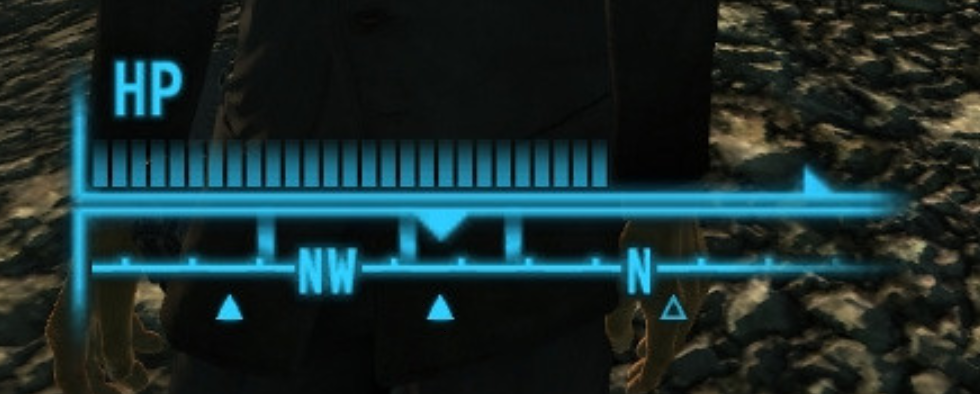
\includegraphics[width=0.9\textwidth]{images/ui/compassSkyrim.png}
	\caption{Kompas z gry Skyrim}\label{fig:Fallout}
\end{figure}


\section{Stawianie budowli (Zofia Sosińska)}\label{chap:omd}
Jedną z kluczowych mechanik gier z gatunku RTS jest budowanie budynków. Funkcjonalność pozwala graczowi 
na podejmowanie strategicznych decyzji w zależności od potrzeb i możliwości budowli. Funkcje pełnione 
przez budynek mogą być bardzo różnorodne. W niektórych przypadkach ich zadaniem jest produkcja surowców, czy leczenie
jednostek, ale są i takie, które skupiają się na wspieraniu w obliczu bitwy. Mogą to być fortyfikacje opóźniające natarcie,
bądź chociażby machiny wojenne towarzyszące ofensywie.

Orcs must die! to strategiczna gra akcji stworzona i wydana przez studio Robot Entertainment. Zadaniem gracza jest wcielenie się
w jednego z  Wojennych Magów i mordowanie nadciągających grup orków za pomocą różnorodnych broni i mechanizmów, które może postawić.
W przejrzysty sposób zostało rozwiązane samo wyświetlenie dostępnych do zbudowania pułapek. Na dole ekranu pokazują się wizerunki mechanizmów,
które może postawić oraz informacja o ich cenie. Naciskając odpowiedni numer na klawiaturze, gracz wybiera, co chce zbudować. Po zatwierdzeniu lewym przyciskiem myszki,
budynek pojawia się w zaznaczonym miejscu. Od tego momentu pułapka będzie pomocą dla głównej postaci podczas zwarcia z przeciwnikami.
Jego ograniczeniem w stawianu mechanizmów są jego fundusze, dlatego musi przemysleć, co kupić oraz gdzie najoptymalniej będzie to postaawić.

\begin{figure}[h!tbp]
    \centering
    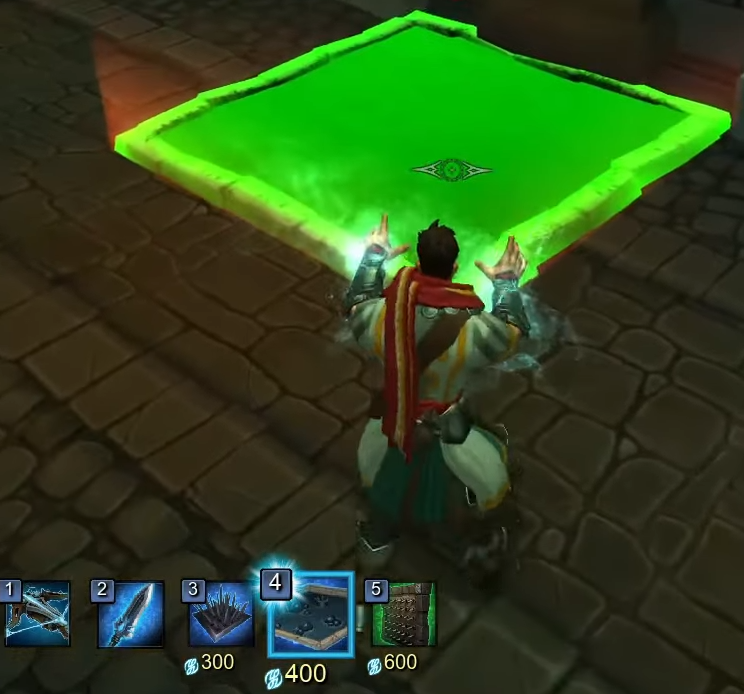
\includegraphics[width=0.9\textwidth]{images/ui/buoildingsOrcs.png}
    \caption{Wyświetlenie dostępnych pułapek w Orcs must die!}\label{fig:Orcs}
\end{figure}
\section{Przekazywanie informacji o świecie w grach (Bartosz Strzelecki)}\label{chap:dbd}
Systemy przekazywania graczowi informacji o świecie są nieocenioną pomocą w kształtowaniu dynamiki i dostarczaniu kluczowych informacji.
Jest to podstawowy element rozgrywki, pozwalający na dynamiczne podejmowanie decyzji oraz na koordynację działań w grach wieloosobowych.

Gra \textit{Dead by Daylight}\footnote{\url{https://deadbydaylight.com}} jest asymetryczną grą wieloosobową, w której gracze wcielają się w rolę postaci "ocalałych" starających się uciec
z mapy albo w rolę "zabójcy", którego celem jest niedopuszczenie do tego. Jednym z udostępnianych przez tę grę mechanizmów jest mechanika widzenia przez przeszkody, która stanowi istotny element rozgrywki, zapewniający
dodatkową warstwę strategii. Polega na wyświetlaniu reprezentacji odległych celów, przedmiotów i przeciwników
zakrytych przez przeszkody. Ta zdolność odgrywa kluczową rolę dla obu stron konfliktu.

W przypadku "ocalałych", ta mechanika jest dostępna dzięki atutom i przedmiotom. Mechanika ujawnia lokalizację celów oraz
innych "ocalałych" pozwalając na koordynację i opracowanie strategii wspólnych działań.

\begin{figure}[h]
\centering
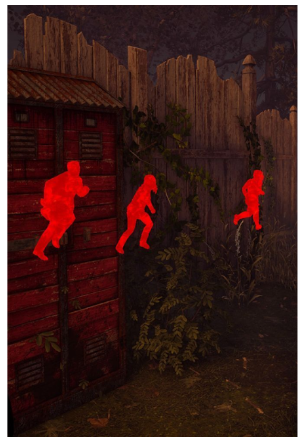
\includegraphics[width=0.4\textwidth]{images/dbd}
\caption{Przykładowy efekt aury w grze \textit{Dead by Daylight}.}
\end{figure}

I odwrotnie, zdolność "zabójcy" do widzenia aury jest kluczowa dla jego mechaniki rozgrywki.
Aury umożliwiają im śledzenie "ocalałych", zwłaszcza gdy korzystają z ich unikalnych mocy lub specyficznych atutów.
Mechanika ta zwiększa napięcie, ponieważ "ocalali" muszą zachować czujność i strategiczne podejście,
aby uniknąć pola widzenia "zabójcy" lub zakłócić ich zdolność czytania aury, aby uciec i osiągnąć cele.

% \begin{figure}[h]
% \centering
% 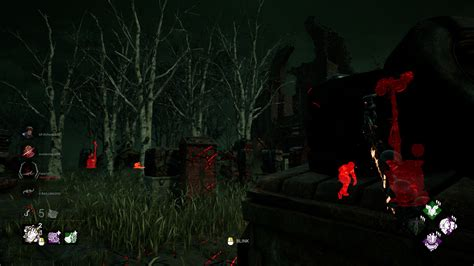
\includegraphics[width=0.6\textwidth]{images/aura}
% \caption{Przykładowe elementy widzenia przez horyzont w grze \textit{Dead by Daylight}.}
% \end{figure}

Ogólnie rzecz biorąc, mechanika aury w \textit{Dead by Daylight} służy jako podstawowy element rozgrywki,
który równoważy wymianę informacji między "ocalałymi" a "zabójcami", znacząco przyczyniając się do atmosfery napięcia i strategii w grze.


\section{Modele celowania w grach (Bartosz Strzelecki)}\label{s:cel}
Celowanie w grach taktycznych jest podstawowym elementem programu, który ma
olbrzymi wpływ na przebieg rozgrywki. Ten mechanizm jest przede wszystkim wykorzystywany
do wzbogacenia gry o kolejną warstwę decyzji taktycznych i zarządzania podejmowanym ryzykiem.
Gracz, przed oddaniem strzału, podejmuje decyzję czy warto zaryzykować podjęcie strzału o niskiej szansie
na trafienie, czy lepiej wykonać niezawodny atak, prawdopodobnie wystawiając się na ataki przeciwników.

W \textit{Phoenix Point}\footnote{\url{https://phoenixpoint.info}} modelowanie celności to wieloaspektowy system, który w zawiły sposób definiuje wynik interakcji bojowych.
Gra wykorzystuje dynamiczny system celowania, który uwzględnia różne elementy, takie jak postawa żołnierza, biegłość w posługiwaniu się bronią, zasięg, 
osłona i warunki środowiskowe, aby określić precyzję strzału. Każdy z tych elementów odgrywa znaczącą rolę w ogólnym obliczeniu trafienia w cel.

W przeciwieństwie do podobnej gry \textit{XCOM}\footnote{\url{https://www.xcom.com}}, gdzie celność jest zamodelowana za pomocą prostej szansy na trafienie, w grze \textit{Phoenix Point}
trajektoria każdego pocisku obliczana jest osobno. Podczas celowania widoczne są dwa okręgi: wewnętrzny, który reprezentuje miejsce,
w którym znajdzie się 50\% pocisków oraz zewnętrzny, który reprezentuje maksymalny rozrzut broni. W tym przypadku im celniejsza broń tym
okręgi będą mniejsze.

\begin{figure}[h]
\centering
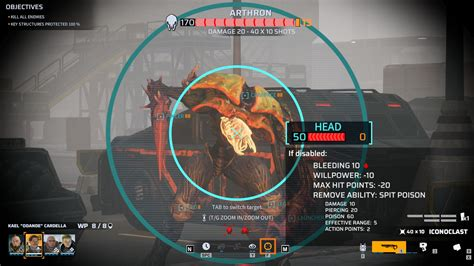
\includegraphics[width=1\textwidth]{images/point}
\caption[System celowania występujący w grze \textit{Phoenix Point}.]{System celowania występujący w grze \textit{Phoenix Point}\protect\footnotemark.}
\label{fig:acc}
\end{figure}
\footnotetext{Internet, \url{https://www.pcgamesn.com/wp-content/uploads/2019/12/phoenix-point-aim.jpg}, dostęp: 16.08.2023}
\FloatBarrier
Ostatecznie system zaimplementowany w grze \textit{Phoenix Point} okazuje się dużo bardziej realistyczny i pozwala na utrzymywanie ciągłej niepewności
co do celności strzału, umożliwiając w ten sposób na strategiczne wyzwania, leżących u podstaw gier tego typu. 


\chapter{Technologie, algorytmy i narzędzia}
W niniejszym rozdziale zostały omówione wykorzystywane w trakcie pracy narzędzia wraz z przeglądem wybranych silników
gier komputerowych. Dodatkowo przedstawiono wykorzystane w projekcie struktury danych .
\section{Przegląd silników gier (Bogna Lew)}\label{s:silniki}
Silnik gier komputerowych jest oprogramowaniem służącym głównie do wytwarzania gier komputerowych. Dostarcza podstawowe
narzędzia, takie jak biblioteki czy edytor poziomów, dzięki którym łatwiej można dokonywać zmian w grze. Wybranie
odpowiedniego silnika przed rozpoczęciem pracy ma kluczowy wpływ na proces wytwórczy i efekt końcowy.

Obecnie dostępnych jest wiele silników, a każdy z nich ma różne możliwości. W celu uproszczenia wyboru zdecydowaliśmy
się zawęzić listę do trzech najpopularniejszych obecnie darmowych silników, czyli Godot, Unity oraz Unreal Engine.

Pierwszy z nich jest w pełni darmowym silnikiem open source. Posiada prosty i intuicyjny interfejs, a w Internecie
tworzone jest przez społeczność wiele samouczków. Nie posiada on jednak oficjalnej dokumentacji oraz jest zdecydowanie
mniej popularny od pozostałych dwóch.

Kolejny silnik, Unity jest określany jako przyjazny dla początkujących. Posiada bogatą dokumentację oraz jest dostępnych
dużo samouczków stworzonych przez jego społeczność. Unity świetnie się nadaje do tworzenia gier 3D. Silnik ten jest
dostępny w wersji bezpłatnej oraz oferującej więcej możliwości wersji płatnej. Co więcej, ma możliwość rozszerzenia
o dodatkowe narzędzia dostępne w Asset Store.

Ostatni z silników jest najbardziej kojarzony z grami AAA. Cechuje go zaawansowana grafika, która umożliwia wytwarzanie
fotorealistycznych gier. Korzystanie z niego jest darmowe, a opłata w wysokości 5\% jest naliczana jedynie, gdy gra
zarobi ponad milion USD.

Tabela \ref{fig:teng} przedstawia porównanie wymienionych silników w istotnych, z punktu widzenia projektu, aspektach.

\begin{table}[h]
\caption{Porównanie silników.}
\begin{center}
\begin{tabular}{ |c||c|c|c| }
 \hline
 Silnik & Unity & Unreal Engine & Godot \\
 \hline \hline
 Popularność & duża & duża & mała \\
 \hline
 3D & Tak & Tak & Tak \\
 \hline
 Język & C\# & C++ & C\#, C++, GDScript \\
 \hline
 Baza wiedzy & dokumentacja, samouczki & dokumentacja, samouczki & samouczki, fora \\
 \hline
 Open source & Nie & Nie & Tak \\
 \hline
\end{tabular}
\end{center}
\label{fig:teng} 
\end{table}

Finalnie zdecydowaliśmy się na implementację gry w Unity, ponieważ jest to silnik, który najlepiej odpowiada wymaganiom projektu.

\subsection{Terrain Toolbox (Bogna Lew)}\label{ss:tTool}
\texttt{Terrain Toolbox} jest narzędziem dostępnym dla silnika Unity. Jest to zasób dostępny w paczce \texttt{Terrain Tools}, który
upraszcza pracę nad modelowaniem terenu do gry.

Do podstawowych funkcjonalności udostępnianych przez \texttt{Terrain Toolbox} należy generowanie terenu na podstawie
map wysokości (ang. \textit{heightmap}) oraz podstawowych parametrów takich jak długość, szerokość i wysokość terenu.
Pozwala to na szybkie utworzenie grywalnej mapy. Ponadto narzędzie \texttt{Terrain Toolbox} umożliwia wygładzenie, dodatkowe
wymodelowanie oraz nałożenie tekstur na tak utworzony teren za pomocą udostępnionych przez nie funkcjonalności.

\begin{figure}[h!]
    \centering
    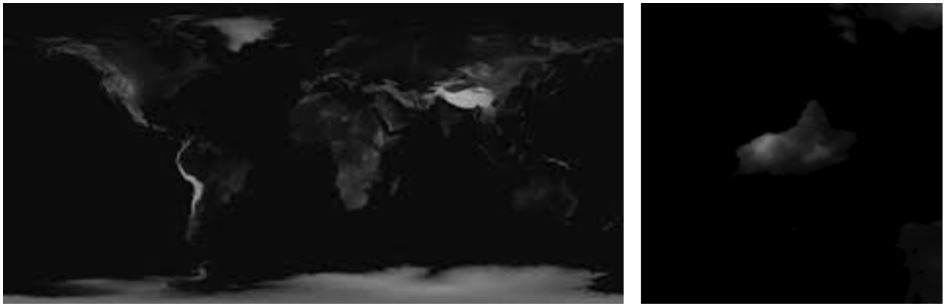
\includegraphics[width=0.8\textwidth]{images/modelowanie_terenu/przykladowe_heightmapy.jpg}
    \caption[Przykładowa mapa wysokości (po lewej) oraz wygenerowany na jej podstawie teren (po prawej).]{Przykładowa mapa wysokości\protect\footnotemark (po lewej) oraz wygenerowany na jej podstawie teren (po prawej).}
\end{figure}
\footnotetext{Internet, \url{https://www.planetminecraft.com/project/isla-nublar-1-1-scale/}, dostęp: 14.06.2023}

Kolejną istotną funkcjonalnością jest malowanie terenu drzewami. Umożliwia ona automatyczne umiejscowienie obiektów na
mapie w losowy sposób. Pozwala to szybko utworzyć realistyczne skupiska obiektów, takich jak las. Poniżej
został przedstawiony przykładowy rezultat.

\begin{figure}[h!]
    \centering
    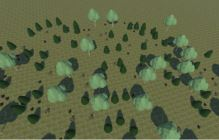
\includegraphics[width=0.7\textwidth]{images/modelowanie_terenu/drzewa.jpg}
    \caption{Widok na teren z drzewami.}
\end{figure}
\FloatBarrier

\subsection{Navmesh (Bartosz Strzelecki)}\label{ss:navmesh}

Komponent Unity \texttt{Navmesh} jest podstawowym elementem wykorzystywanym w przypadku znajdywania ścieżek.
Jest to mechanizm pozwalający na przechowywanie wyspecjalizowanych danych, które reprezentują
powierzchnie, po których mogą poruszać się agenty sztucznej inteligencji.
W skrócie \texttt{NavMesh} to "Siatka generowana przez Unity w celu przybliżenia obszarów, po których można chodzić i przeszkód w
otoczeniu, w celu znalezienia ścieżki i nawigacji kontrolowanej przez sztuczną inteligencję" \cite{unity}.

Aby zacząć korzystać z komponentu należy wygenerować mapę w edytorze Unity.
W ramach tego procesu wykonywane są obliczenia mające na celu wykrycie powierzchni,
po której może poruszać się dany agent. Ten system bierze pod uwagę kąt nachylenia
powierzchni, szerokość przejścia, jak i wysokość stropu.

W trakcie rozgrywki komponent \texttt{NavMesh Agent} wykorzystuje wcześniej wygenerowane dane
do wyznaczenia najlepszej ścieżki do celu. Z poziomu skryptów można dynamicznie modyfikować powierzchnię
nawigacyjną, umożliwiając w ten sposób uzyskanie poruszających się przeszkód i dynamicznie powstających budynków.

\begin{figure}[h!]
    \centering
    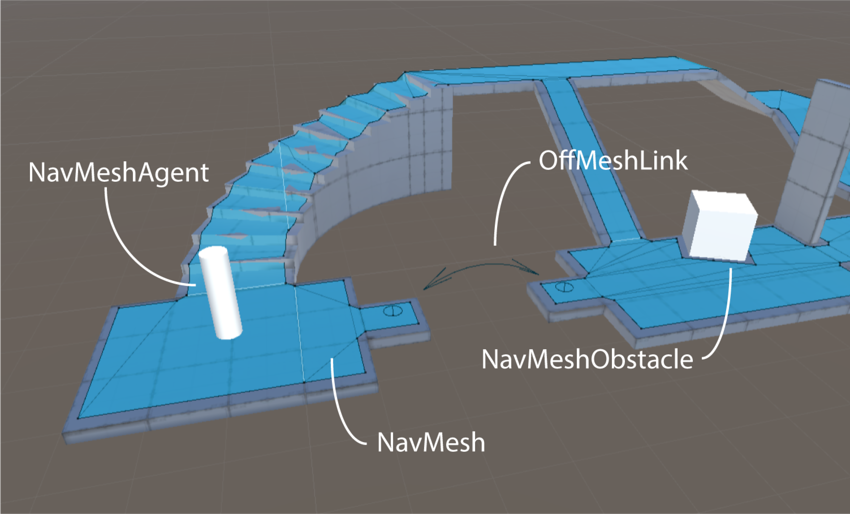
\includegraphics[width=0.7\textwidth]{images/navmesh.png}
    \caption{System nawigacji w Unity.}
\end{figure}

Podsumowując, system \texttt{NavMesh} istotnie upraszcza zadanie odnajdywania ścieżki, co pozwala na łatwe zaimplementowanie
realistycznych zachowań agentów sztucznej inteligencji. Znacznie ułatwia też zadanie tworzenia świata gry ze względu na automatyczny
sposób generowania danych nawigacyjnych.



\chapter{Projekt systemu}\label{chap:projekt}

W tym rozdziale został przedstawiony zamysł członków zespołu na opracowywaną grę. Stanowi on opis pożądanych rezultatów,
do których zespół będzie dążyć w trakcie implementacji. Kolejno zostały opisane oczekiwane działanie poszczególnych
mechanik, z których będzie się składał ostateczny produkt. 
\section{Organizacja (Bartosz Strzelecki)}\label{s:org}
W tym podrozdziale przedstawiono harmonogram prac, wraz z ich przewidywanym terminem realizacji.
Ponadto zaprezentowano skład zespołu projektowego, kompetencje ich członków oraz podział zadań.
\subsection{Główne etapy projektu}
\begin{center}
  \begin{tabular}{| m{30em} | m{12em}|} 
  \hline
  Etap & Termin realizacji \\
  \hline\hline
  Wybór i analiza konkretnego kontekstu historycznego. & Kwiecień 2023 \\
  \hline
  Syntetyczny opis modelu postrzegania przestrzeni na podstawie dzieł pisanych, architektury i sztuki. & Kwiecień — Maj 2023 \\
  \hline
  Przegląd rozwiązań stosowanych w grach strategicznych z wybranego okresu oraz dodatkowo mechanizmów z innych gier, które mogłyby być zaadoptowane na potrzeby projektu. & 2, 3 kwartał 2023 \\
  \hline
  Opracowanie fabuły, selekcja postaci i wydarzeń, a także określenie zakresu autonomii świata gry oraz możliwości modyfikowania go przez gracza. & Czerwiec 2023 \\
  \hline
  Opracowanie szczegółowej koncepcji i projektu gry, w tym projekt mechanizmów zawartych w prototypie. & Lipiec 2023 \\
  \hline
  Implementacja poszczególnych funkcjonalności gry. & 4 kwartał 2023 \\ 
  \hline
  Testowanie, weryfikacja założeń i walidacja. & Listopad — Grudzień 2023 \\
  \hline
  Stworzenie dokumentacji przeprowadzonych prac. & 3, 4 kwartał 2023 \\
  \hline
\end{tabular}
\end{center}
Przewidywany termin zakończenia prac nad projektem to grudzień 2023 roku.
\begin{figure}[htbp]
    \centering
    \includegraphics[width=1\textwidth]{uml/Harmonogram}
    \caption{Harmonogram przedstawiony w postaci diagramu gantt.}
\end{figure}
\break
\section{Skład zespołu projektowego}
\begin{center}
  \begin{tabular}{ | m{10em} || m{10em} | m{10em} | m{10em} | }
    Imię i nazwisko & Bogna Lew & Zofia Sosińska & Bartosz Strzelecki \\
  \hline\hline
    Numer indeksu & 184757 & 184896 & 184529 \\
  \hline
    %%Kompentencje & Posiada & Posiada & Posiada \\
    Zadania & System budowania, sterowanie postacią & Interfejs użytkownika & Sztuczna inteligencja postaci\\
  \hline
  \end{tabular}
\end{center}

\section{Analiza i specyfikacja wymagań (Bogna Lew)}\label{s:wymagania}
W niniejszej sekcji przedstawiono specyfikę wymagań funkcjonalnych, pozafunkcjonalnych oraz tych, wynikających z
głównych założeń projektu. Dodatkowo zawiera ona diagramy przypadków użycia, maszyny stanów oraz klas prototypowej gry.

\subsection{Specyfika wymagań wynikających z założeń projektu}
“Starożytni świat widzieli inaczej, mniej płasko”\cite{gbobrektvgry}. Dobrze obrazującym ówczesne postrzeganie
przestrzeni przykładem jest mapa Imperium Rzymskiego, pokazana na \ref{fig:mapaIR}. Czytanie jej dosłownie mija się z
celem. Nie są na niej zachowane ani proporcje, ani strony świata. Mimo tego, że basen Morza Śródziemnego został
ówcześnie dosyć dokładnie oddany, “nie wydaje się, aby Rzymianom współczesna kartograficzna wierność była potrzebna”\cite{gbobrektvgry}.
“Dowódcy opierali się na swojej wiedzy, wiedzy wynajętych przewodników oraz informacjach zwiadowców i tubylców”\cite{gbobrektvgry}.

\begin{figure}[htbp]
    \centering
    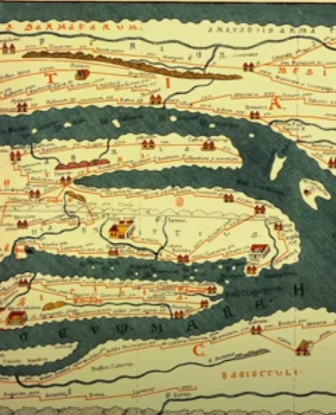
\includegraphics[width=0.5\textwidth]{images/mapaIR.png}
    \caption{Mapa basenu Morza Śródziemnego z czasów Imperium Rzymskiego}\label{fig:mapaIR}
\end{figure}

Z punktu widzenia projektu kluczowe jest jak najdokładniejsze oddanie realiów historycznych przy jednoczesnym
uwzględnieniu jakości rozgrywki gracza oraz cech charakterystycznych dla gier typu RTS. Z założeń wynika, że fabuła
gry powinna zostać osadzona w czasach sprzed wielkich odkryć geograficznych. Na tej podstawie zostały zdefniowane
dodatkowe wymagania, które powinien spełniać prototyp:
\begin{itemize}
  \item Sposób nawigacji powinien jak najdokładniej odpowiadać temu stosowanemu w wybranej epoce;
  \item Postacie w grze powinny stylistycznie pasować do realiów historycznych;
  \item Postacie powinny posługiwać się słownictwem adekwatnym do czasów, w których osadzona jest gra;
  \item Postacie powinny jak najlepiej oddawać światopogląd w danych czasach;
  \item Oręż stosowany w grze powinien odpowiadać realiom historycznym;
  \item Budowle w grze powinny stylistycznie odpowiadać wybranej epoce;
  \item Sposób komunikacji z postaciami powinien imitować ten stosowany w danych czasach;
\end{itemize}

\subsection{Wymagania funkcjonalne}\label{ss:fun}
W przedstawionej liście zostały wymienione wymagania funkcjonalne, które powinien spełniać prototyp gry.

\begin{itemize}\label{list:fun}
  \item Zapis oraz odczyt wybranego stanu gry lokalnie na komputerze użytkownika;
  \item Uruchomienie nowej gry;
  \item Możliwość sterowania postacią gracza;
  \item Możliwość nawigacji w świecie gry;
  \item Możliwość wchodzenia w interakcję z postaciami niezależnymi;
  \item Możliwość przyjmowania zleceń od postaci niezależnych;
  \item Możliwość najmowania postaci wojowników;
  \item Możliwość wydawania komend wynajętym postaciom;
  \item Możliwość zlecania budowy;
  \item Możliwość zdobywania zasobów;
\end{itemize}

\subsection{Wymagania pozafunkcjonalne}\label{ss:nonfun}
Poniższa lista przedstawia wymagania niefunkcjonalne projektu.

\begin{itemize}\label{list:nonfun}
  \item Rozgrywka w trybie offline;
  \item Działanie na urządzeniach z systemem Windows lub Linux;
  \item Dostosowywanie rozmiaru do wielkości ekranu komputera użytkownika;
  \item Obsługa klawiatury oraz myszy;
  \item Działanie w czasie rzeczywistym;
\end{itemize}

\subsection{Diagram przypadków użycia}\label{ss:usecase}
Niniejsza sekcja przedstawia diagram przypadków użycia dla głównych funkcjonalności, które będzie zawierać prototypowa gra.
Opisuje on przewidywane usługi oferowane przez poszczególne mechaniki programu.

Jedną z głównych akcji, które gra udostępnu jest wydanie rozkazów przyjaznym jednostkom. Polega ona na poinformowaniu
wojowników przez gracza jaką czynność powinni w danym momencie wykonać. Kolejną możliwością jest zlecenie budowy, czyli
poelceniu postaci budowniczego wybudowania wybranego obiektu w określonym przez gracza miejscu. Ponadto użytkownik
będzie mógł przeprowadzać rozmowy z postaciami niezależnymi. Oznacza to, że będzie mógł zainicjować z nimi dialog i
następnie kształtować jego przebeig poprzez wybieranie swoje odpowiedzi z opcji proponowanych przez grę.

\begin{figure}[!htbp]
    \centering
    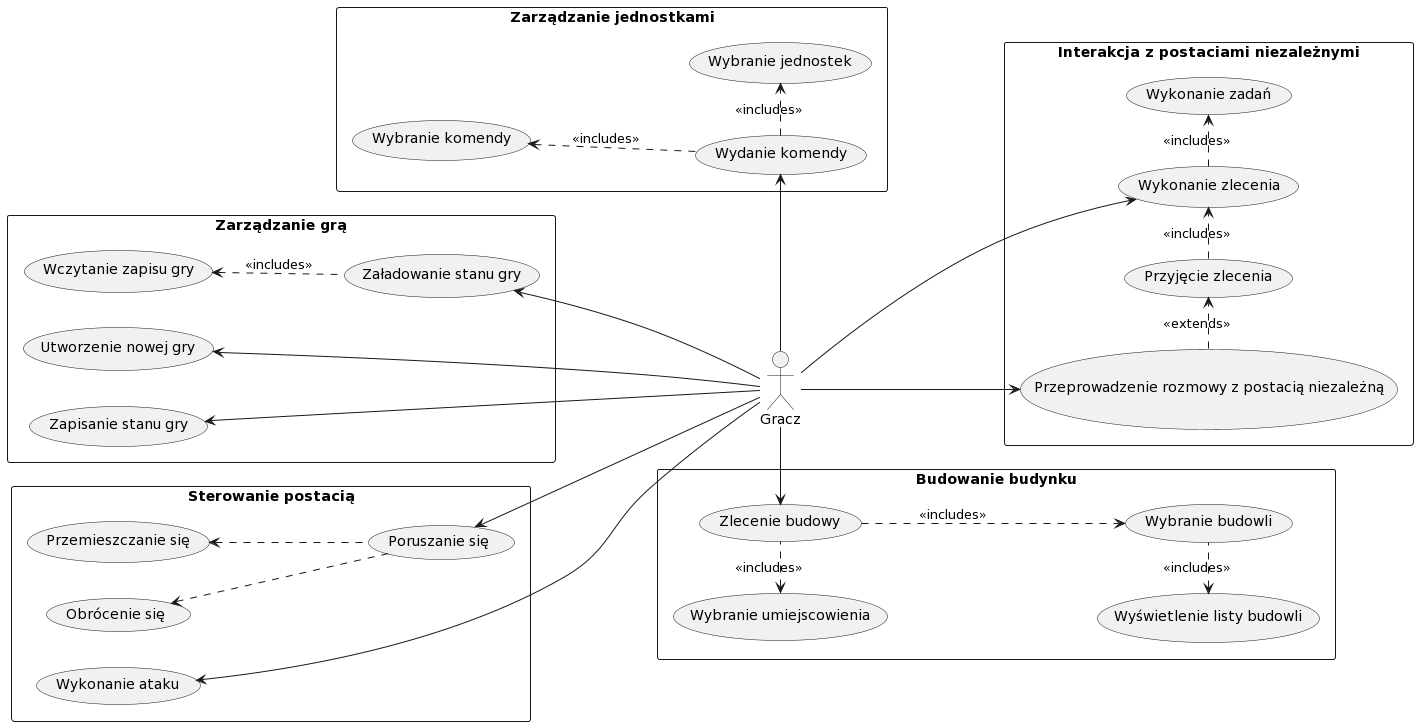
\includegraphics[width=1.0\textwidth]{images/diagrams/usecase.jpg}
    \caption{Diagram przypadków głównych mechanik gry.}\label{fig:usecases}
\end{figure}
\FloatBarrier

\subsection{Diagram stanów}\label{ss:state}
W tym podpunkcie został przedstawiony diagram stanów prototypowej gry, który ukazuje jej przewidywany sposób działania.
Prezentuje on podstawowe stany, w których może się znaleźć system gry.

Do podstawowych stanów należą "Menu główne" oraz "Rozgrywka". Pierwszy z nich oznacza, że program został uruchomiony, a
gracz wyświetla panel główny. Z tego stanu możliwe jest przejście do stanów "Odczytanie stanu gry" bądź "Utworzenie
nowej gry", które to powodują rozpoczęcie gry z zapisu lub od początku.

Stan "Rozgrywka" jest stanem złożonym i określa, że gra została rozpoczęta. W jego skład wchodzą przede wszytskim takie
stany jak "Interakcja z postacią niezależną", w którym program się znajdzie gdy gracz rozpocznie dialog z postacią w grze,
czy "Zarządzanie jednostkami", który to oznacza, że użytkownik wydaje rozkazy swoim wojownikom.

Diagram stanów został przedstawiony na rysunku \ref{fig:states}.

\begin{figure}[!htbp]
    \centering
    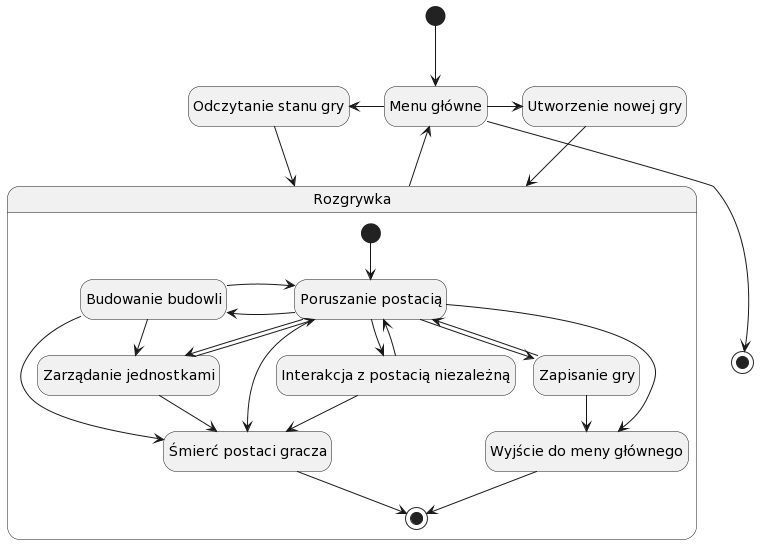
\includegraphics[width=1.0\textwidth]{images/diagrams/state.jpg}
    \caption{Diagram stanów gry.}\label{fig:states}
\end{figure}
\FloatBarrier

\subsection{Diagram klas}\label{ss:class}
W tej sekcji został pokazany uproszczony diagram klas (rys. \ref{fig:classes}), przedstawiający główne elementy gry.
Obrazuje podstawową strukturę tworzonego systemu oraz zależności pomiędzy poszczególnymi komponentami.

Do najważniejszych klas należą "Interfejs użytkownika", "Mechanizm interakcji z postaciami", "Mechanizm zarządzania
jednostkami" oraz "Mechanizm budowania". Obrazują one podstawowe komponenty gry, których głównym zadaniem jest zarządzanie
poszczególnymi mechanikami. "Interfejs użytkownika" jest odpowiedzialny za interakcję z graczem oraz pomaganie mu w
trakcie rozgrywki. Pozostałe trzy odpowiadają kolejno za umożliwienie graczowi na prowadzenie dialogów z postaciami
niezależnymi, wydawanie komend jego zaprzyjaźnionym jednostkom oraz budowanie obiektów.
\begin{figure}[!htbp]
    \centering
    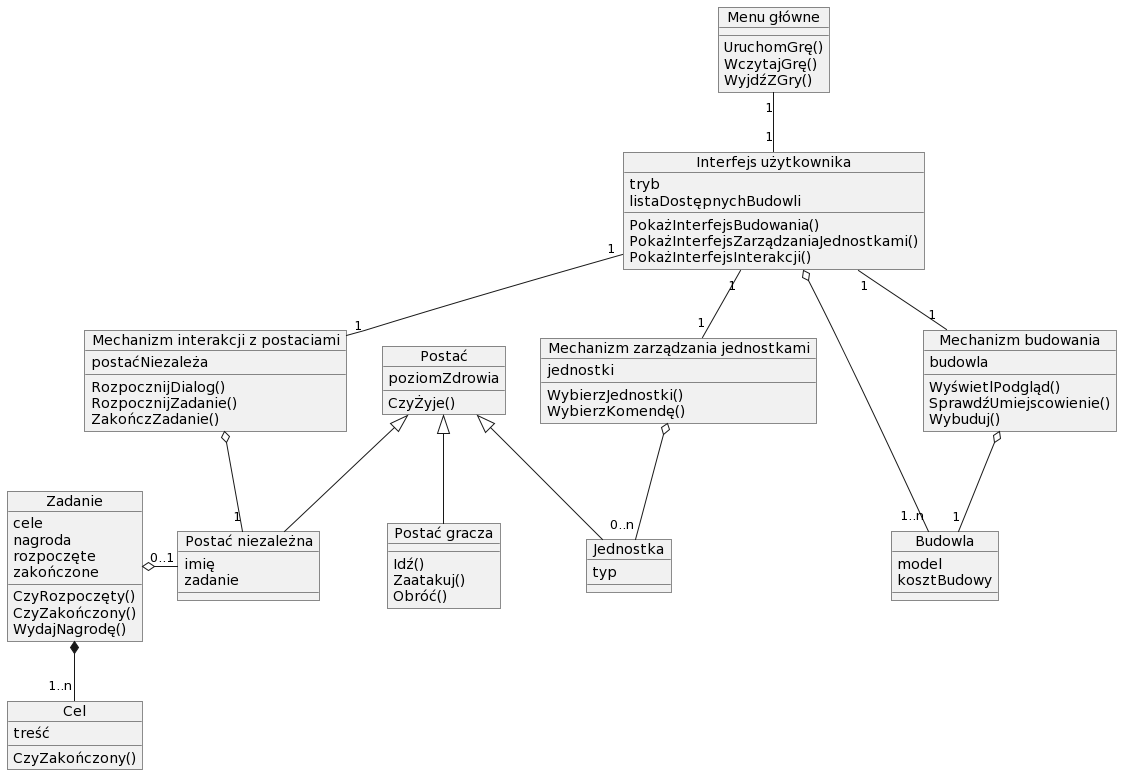
\includegraphics[width=1.0\textwidth]{images/diagrams/class.jpg}
    \caption{Diagram klas gry.}\label{fig:classes}
\end{figure}
\section{Opis świata gry (Bogna Lew)}
Fabuła wytwarzanej gry ma zostać osadzona w realiach wczesnośredniowiecznych. Została ona zainspirowana Celtami, których
w tym okresie można było spotkać głównie w Irlandii. Z tego powodu mapa świata gry będzie prezentować górzystą wyspę, na
której gracz będzie mógł znaleźć niewielką wioskę oraz obozowiska.

Graczowi udostępniona zostanie jego własna postać do bezpośredniego sterowania. Takie rozwiązanie "czyni gracza
kreatywnym elementem działajacym wewnątrz dyskursu, który posiada przestrzenny charakter"\cite{olbrzymwcieniu}. Typowym
elementem gry są zadania poboczne, czasem pośrednio związane z głównym celem gry. Stanowi to urozmaicenie rozgryki i
dodatkowo zachęca gracza do zagłębiania się w nią. "W odniesieniu do gier komputerowych można więc mówić o podwójnym
motywowaiu ich użytkowników, które dokonuje sie na dwóch narracyjnych poziomach: jedna z motywacji wyznacza cel całej
rozgrywce, druga natomiast jest ulokowana w przestrzeni pojedynczej misji i kończy wraz z jej zakończeniem"\cite{olbrzymwcieniu}.
Z tego powodu trakcie gry użytkownik będzie mógł spotkać postaci niezależne, z którymi możliwe będzie wejście w interakcje, kończące
się np. zleceniem wykonania zadania. W ich realizacji będą mu pomagać jednostki, z którymi się zaprzyjaźni w trakcie
rozgrywki i którym będzie mógł wydawać komendy zgodnie z ich typem. Dodatkowo w trakcie eksploracji świata natrafi na
nieprzyjazne postacie, z którymi będzie toczyć walki. Grę urozmaicą postaci zwierząt, które mogą być neutralne, bądź
agresywne wobec gracza.

Gra będzie udostępniać trzy podstawowe surowce, za które gracz będzie mógł budować budynki. Przewidywane są dwa sposoby
ich pozyskiwania. Pierwszym z nich jest wykonywanie zadań, za które może uzyskać nagrody w postaci pewnej ilości
surowców. Kolejnym sposobem jest zbieranie kłód drewna oraz kamieni leżących na ziemi. Podnoszenie ich dostarczy
jednorazowy przypływ odpowiadającego im zasobu.

\section{Interfejs użytkownika (Zofia Sosińska)}\label{chap:ui}
Interfejs użytkownika (ang. user interface, UI) jest to zbiór najważniejszych informacji przedstawiony graczowi w sposób czytelny. Może się to odbywać za pomocą na przykład obrazków, tekstów, czy wskaźników. Dzięki UI możliwy jest wgląd w aktualny stan wiedzy grywalnej postaci. 

Projekt interfejsu użytkownika przewiduje trzy tryby: zwykły, budowania oraz walki. Zadaniem każdego z nich będzie odzwierciedlenie aktualnej wiedzy granej postaci z naciskiem na najpotrzebniejsze w danej chwili informacje.
	
\subsection{Interfejs podstawowy}
Interfejs podstawowy przewiduje funkcje, takie jak pokazanie:
\begin{itemize}
    \item surowców i funduszy,
    \item aktualnego czasu w grze, 
    \item kompasu,
    \item informacji o możliwym  rozpoczęciu konwersacji z inną postacią;
\end{itemize}
Inspiracją dla górnego paska z informacjami jest ten użyty w grze Warcraft 3. Prostota i surowość stylu będą współgrać z klimatem gry.

W naszej grze skupimy się jednak na tym, aby interfejs użytkownika zabierał jak najmniej miejsca. Dlatego też projekt zakłada, że poszczególne obiekty nie będą ze sobą połączone, a jedynie “dryfować” w przestrzeni.
Jako ważny element tej części UI zawarty zostanie kompas, wzorowany na tym z gry The Elder Scrolls V: Skyrim.


Szacowany projekt interfejsu podstawowego UI wyświetlono na rysunku \ref{fig:ui_main} .
\begin{figure}[htbp]
    \centering
    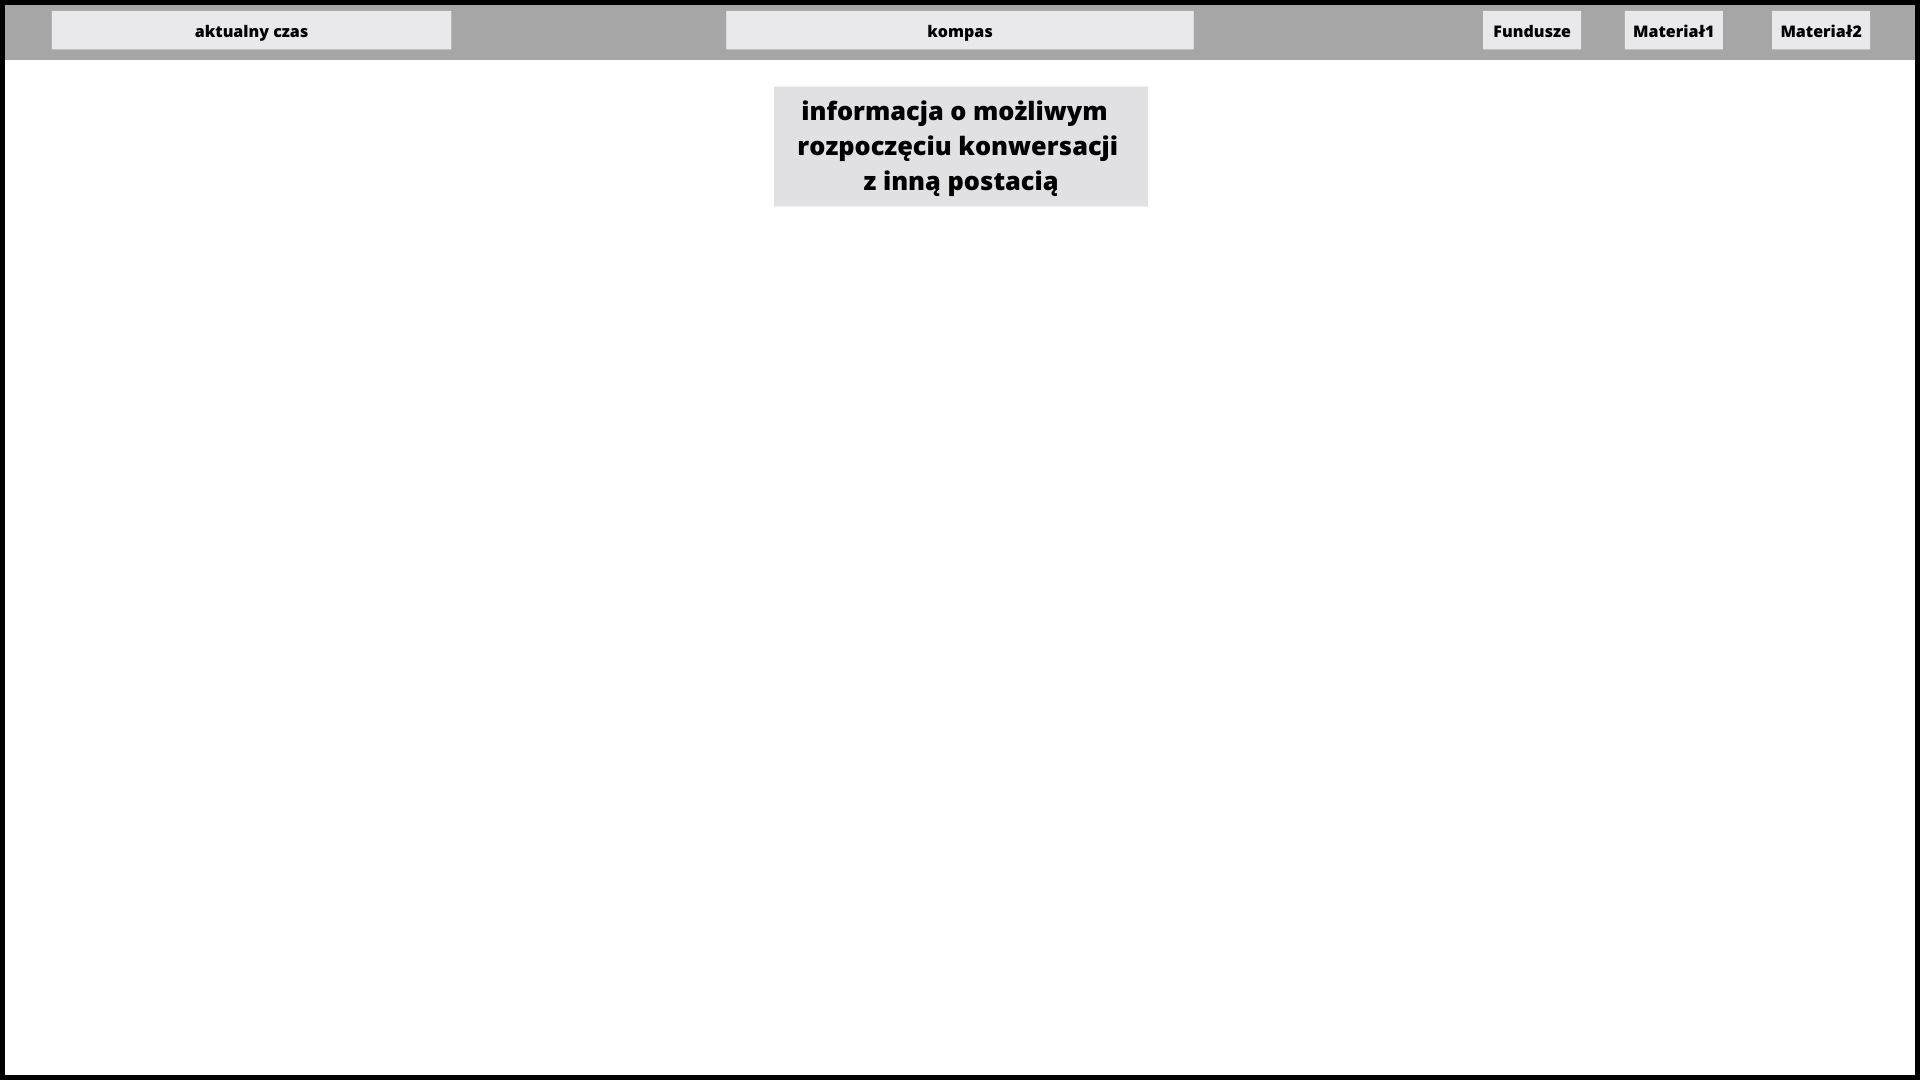
\includegraphics[width=0.9\textwidth]{images/ui/ui_proj_ogolne.jpg}
    \caption{Projekt interfejsu podstawowego UI.
    }\label{fig:ui_main}
\end{figure}
 
\subsection{Menu stawiania budynków}
 W menu stawiania budynków informacje wcześniej przedstawione zostaną na ekranie. Dodatkowo pokażą nam się dostępne do zbudowania budynki, a po wybraniu pojawią się przed nami. Po zatwierdzeniu budynek zostanie wybudowany.
	Inspiracją do przedstawienia dostępnych budowli jest rozwiązanie gry Orcs must die!


    Szacowany projekt trybu budowania UI wyświetlono na rysunku \ref{fig:ui_bud} .
    \begin{figure}[htbp]
        \centering
        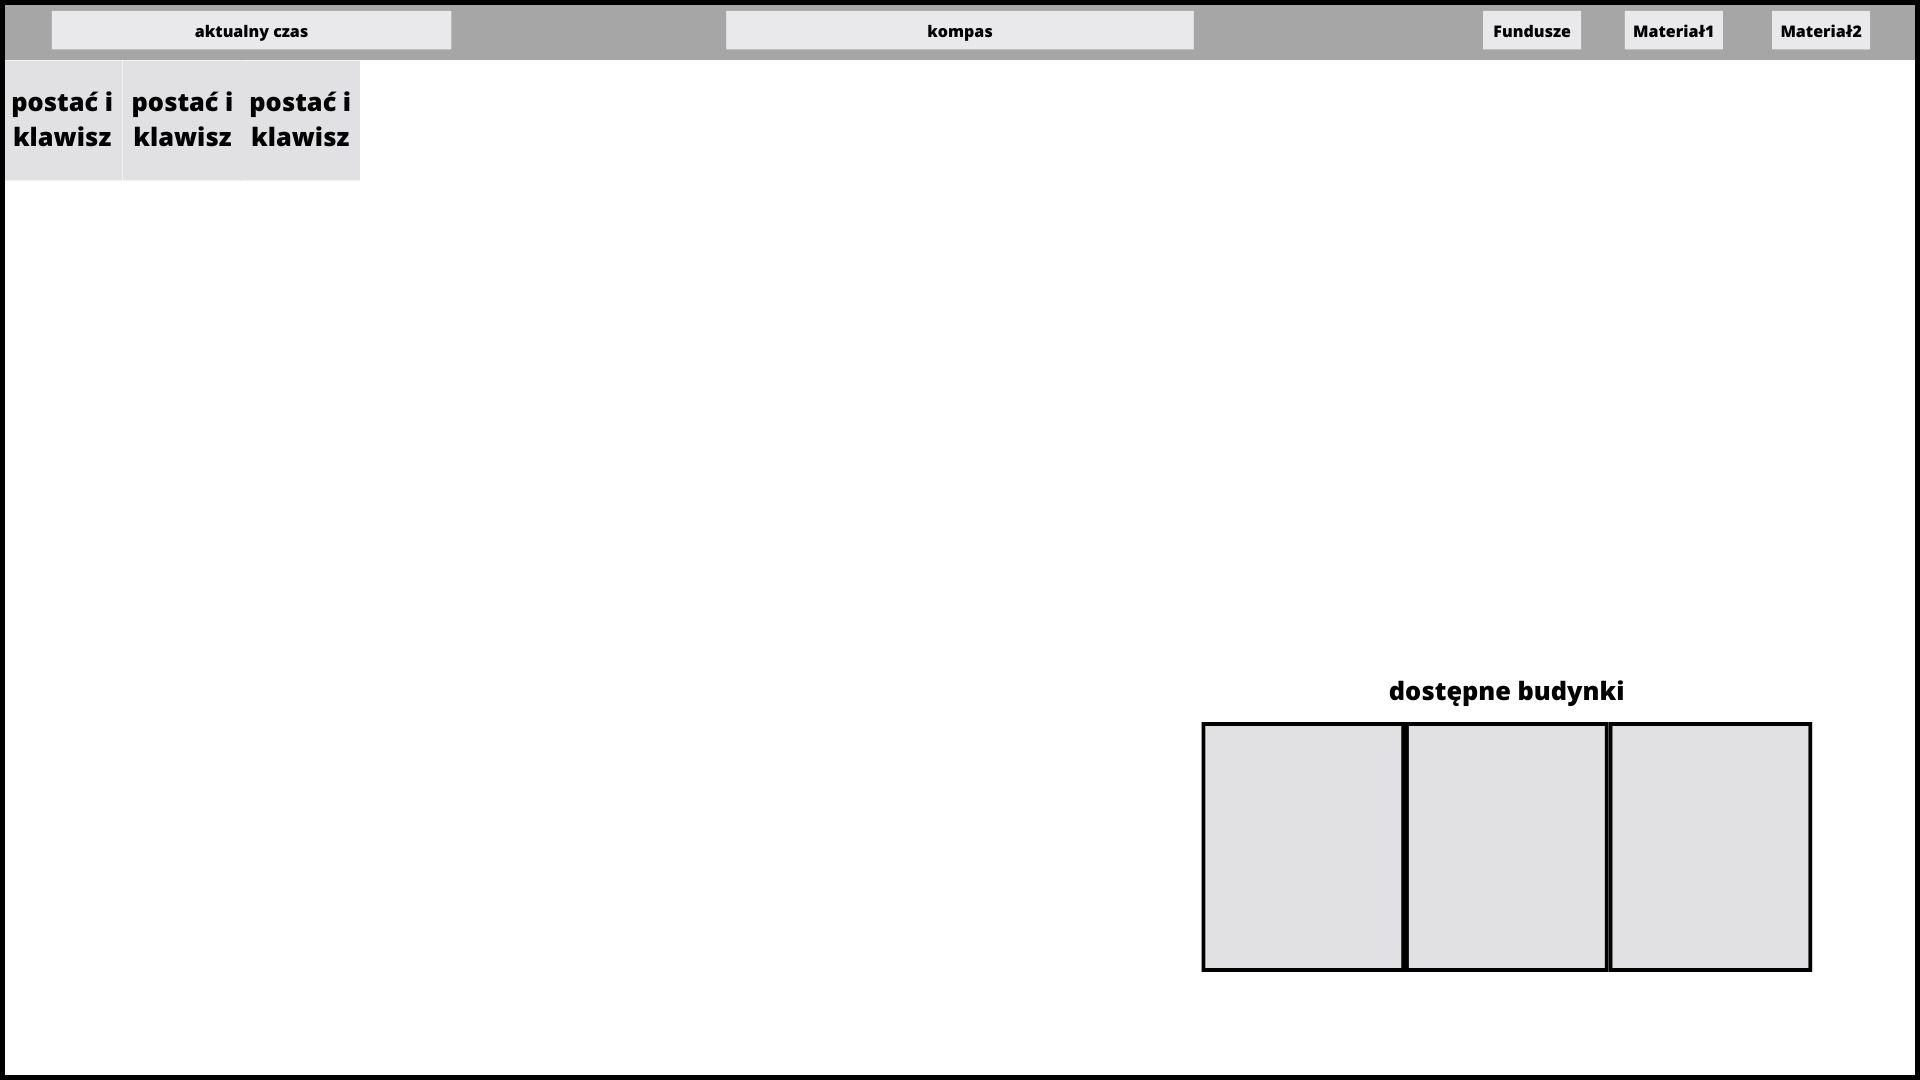
\includegraphics[width=0.9\textwidth]{images/ui/ui_proj_budowanie.jpg}
        \caption{Projekt menu stawiania budynków UI.
        }\label{fig:ui_bud}
    \end{figure}


\subsection{Tryb walki}
Bliźniaczo do trybu budowania, gdy rozpocznie się walka, podstawowe informacje zostają na ekranie, a dodatkowo gracz dostaje informacje o dostępnych rozkazach do wydania. Nasze rozwiązanie będzie podobne do pomysłu z gry Mount\&Blade.

Szacowany projekt trybu budowania UI wyświetlono na rysunku \ref{fig:ui_wal} .
    \begin{figure}[htbp]
        \centering
        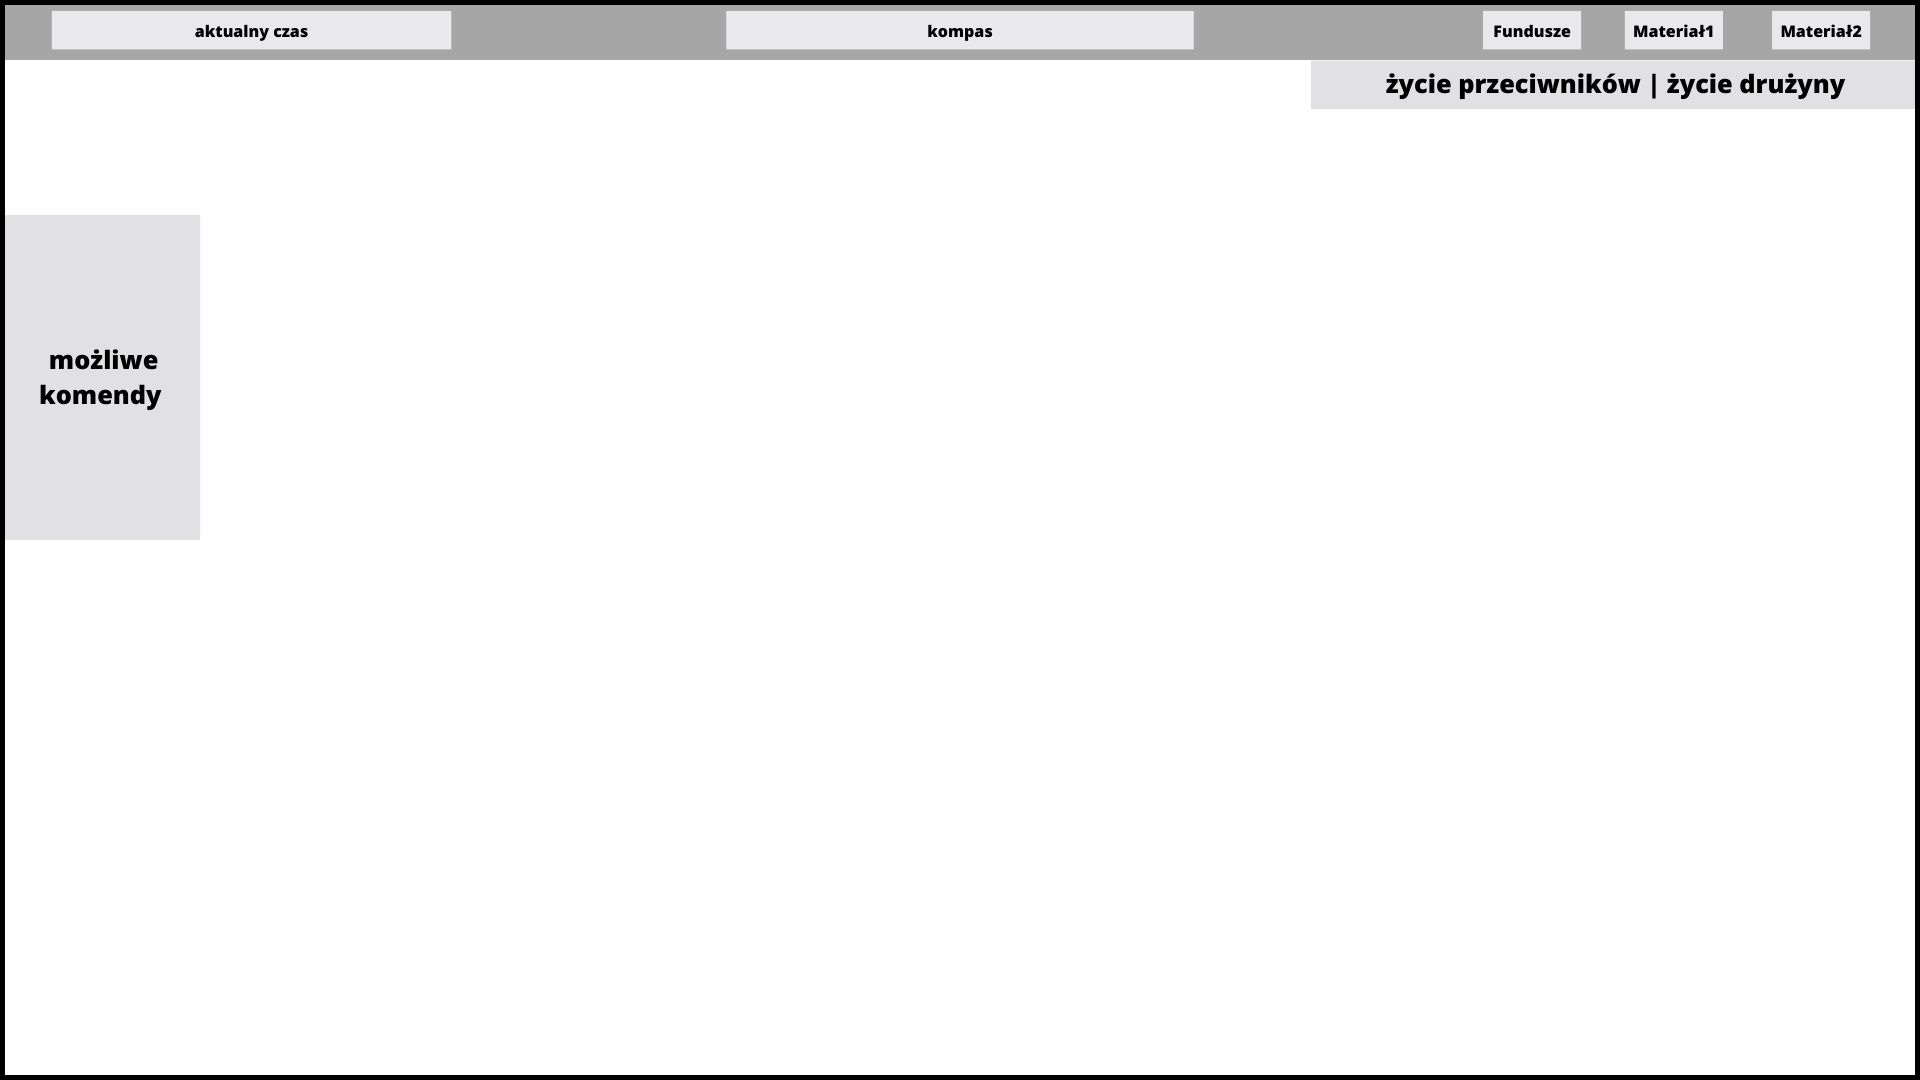
\includegraphics[width=0.9\textwidth]{images/ui/ui_proj_walka.jpg}
        \caption{Projekt trybu walki UI.
        }\label{fig:ui_wal}
    \end{figure}

\section{Nawigacja (Zofia Sosińska)}\label{chap:naw}

Kluczowym dla gry założeniem jest ułatwienie graczowi wczucia się w realia świata, w którym się znajduje. 
Jako jeden z głównych warunków pogłębienia immersji uwypuklono brak implementacji mapy, na której gracz widziałby świat. 
W ten sposób nie upraszczamy mu poruszania się i odnajdywania lokacji tak,
jak i człowiek w realnym świecie w czasach średniowiecznych nie kierował się zapisanymi na kartce kartograficznymi obrazami, 
ale własną i zdobytą od innych wiedzą o otaczającym go terenie. 

Jedyną pomocą, jaką otrzyma gracz, będzie pasek obrazujący pole widzenia granej postaci.
Pierwszą rolą narzędzia będzie pokazanie kierunku świata, który znajduje się w polu widzenia gracza.
Zakładamy, że grana postać potrafi sama taką informację odczytać, chociażby z położenia Słońca.

Kolejną informacją na omawianym elemencie będzie miejsce, w którym znajduje się przeciwnik. 
Dotyczy to antagonistów widocznych w polu widzenia, jak i ukrytych za ścianą. 
Druga część będzie logicznie ponieważ zakładamy, że postać gracza może usłyszeć 
wroga za przeszkodą.


\section{Mechanizm budowania (Bogna Lew)}\label{s:bud_impl}

Opracowany mechanizm umożliwia graczowi na przełączenie się w tryb budowania poprzez naciśnięcie klawisza \texttt{B}, który od razu
wyświetli podgląd bazowego obiektu. Widok budynku przemieszcza się przed postacią oraz odpowiednio obraca się razem z
nią. Efekt poruszania się podglądu został uzyskany za pomocą poniższego wzoru:
\begin{equation}
\begin{cases}
x = r \times sin(\alpha) \\
y = 0 \\
z = r \times cos(\alpha)
\end{cases}
\end{equation}

gdzie $x$, $y$ i $z$ to współrzędne odpowiednio względem osi X, Y i Z, $r$ to odległość środka obiektu od postaci
gracza, natomiast $\alpha$ to kąt o jaki jest on obrócony względem osi Y.

Podgląd budynku będzie widoczny do czasu, aż gracz go umieści naciskając prawy przycisk myszy bądź wychodząc z trybu
edycji naciskając klawisz \texttt{Escape}. Jeżeli widok budowli znajduje się w poprawnym do umieszczenia miejscu to jest on
podświetlany na zielono, w przeciwnym razie - na czerwono. Wybudowanie powoduje przywrócenie bazowych kolorów obiektu
oraz włącza wykrywanie kolizji z nim, dzięki czemu budynek poprawnie oddziałuje z otaczającym go środowiskiem.

\begin{figure}[h!]
    \centering
    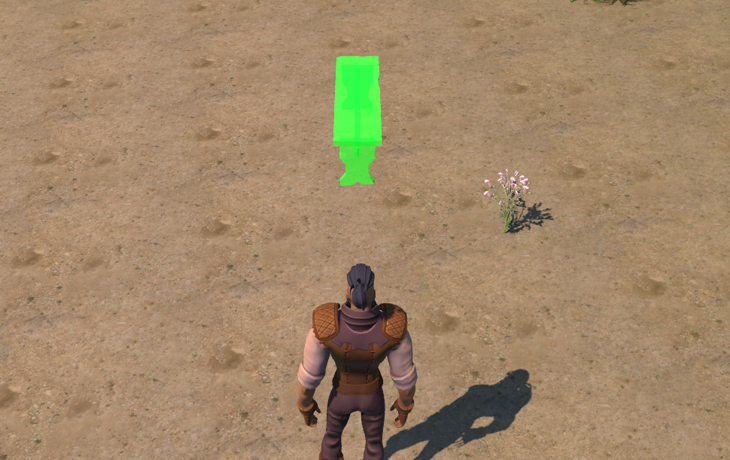
\includegraphics[width=1\textwidth]{images/implementacja/mechanizm_budowania/poprawne.png}
    \caption{Przykład podglądu w poprawnym umiejscowieniu.}
\end{figure}
\FloatBarrier

Do weryfikacji poprawności umiejscowienia budynku wykorzystano mechanizmy wyzwalacza (ang. \textit{trigger}) oraz rzucania
promienia (ang. \textit{raycasting}). Pierwszy z nich polega na wykrywaniu czy obiekt znalazł się w obszarze kolizji bez
brutalnego zatrzymywania go. Oznacza to, że może on przeniknąć przez inny element bez widocznych konsekwencji, jedynie
wysyłając sygnał, że dana sytuacja nastąpiła. Druga metoda natomiast polega na wypuszczeniu promienia o pewnej długości
w zadanym kierunku i sprawdzeniu, czy z czymś się zderzył.

Wyzwalacz został zastosowany do wykrywania kolizji z innymi obiektami na mapie, takimi jak postacie, czy elementy
scenerii niebędące terenem. W tym celu wykorzystano metody \verb|OnTriggerEnter()| i \verb|OnTriggerExit()|, które są wywoływane
odpowiednio gdy, dany obiekt znalazł się w obszarze kolizji innego elementu, bądź go opuścił. Każda z nich odpowiednio
zmienia poprzez zwiększenie bądź zmniejszenie wartości licznika kolizji obiektu. Jeżeli jego wartość jest różna od zera, tzn.
obiekt z czymś koliduje, to umiejscowienie jest uznawane za niepoprawne.

Drugi z mechanizmów został wykorzystany do sprawdzenia nachylenia podłoża. Efekt został osiągnięty poprzez rzucenie
promienia o niewielkiej długości z każdego z dolnych narożników obiektu i zliczeniu ile z nich wykryło kolizję z ziemią.
Brak wykrycia kolizji można zinterpretować jako zapadanie się bądź zbyt mocne lewitowanie danego narożnika nad
powierzchnią ziemi. Z tego powodu przyjęto, że jeśli co najmniej trzy z nich zderzyły się z podłożem, to umiejscowienie
jest poprawne.

\begin{figure}[h!]
    \centering
    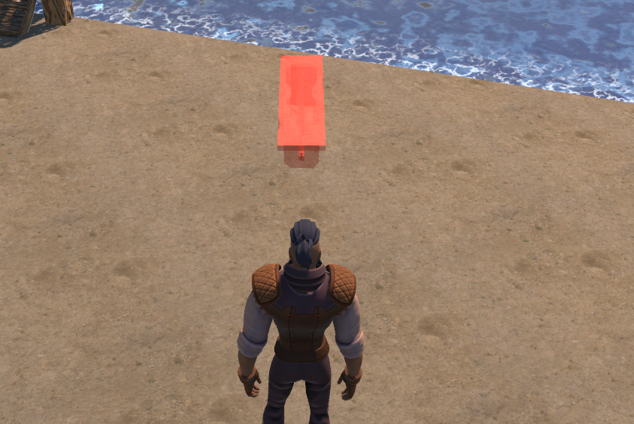
\includegraphics[width=1\textwidth]{images/implementacja/mechanizm_budowania/niepoprawne.png}
    \caption{Przykład podglądu w niepoprawnym umiejscowieniu.}
\end{figure}
\FloatBarrier

Dodatkowo metodę rzucania promienia wykorzystano do wykrycia kolizji z drzewami. Obiekty te są traktowane przez silnik
jako część terenu, przez co metoda wykorzystująca wyzwalacz pomija je. Dlatego w celu wykrywania kolizji z nimi
zdecydowano się na rzucenie dwóch grup promieni biegnących w głąb obiektu z naprzeciwległych krawędzi prostopadłych do
osi Y. Każdy z promieni biegnie w połowie wysokości obiektu i sięga przeciwnej ściany. Tak skomplikowany układ ma na
celu zapewnienie poprawności wykrywania kolizji w przypadku, gdy początki promieni znajdują się wewnątrz kolidującego
obiektu. Jeśli którykolwiek z nich zderzy się z drzewem, to wybrane miejsce jest uznawane za niepoprawne.

\begin{figure}[h!]
   \centering
   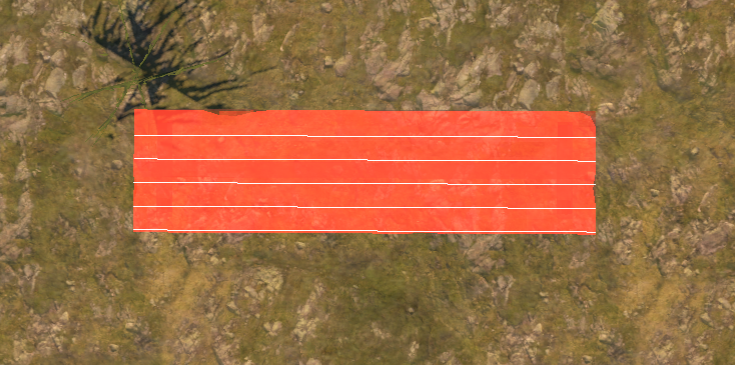
\includegraphics[width=1\textwidth]{images/implementacja/mechanizm_budowania/gizmos_drzewo_2.png}
   \caption{Widok z góry na siatkę promieni służących do wykrywania kolizji z drzewami.}
\end{figure}
\FloatBarrier
\begin{figure}[h!]
   \centering
   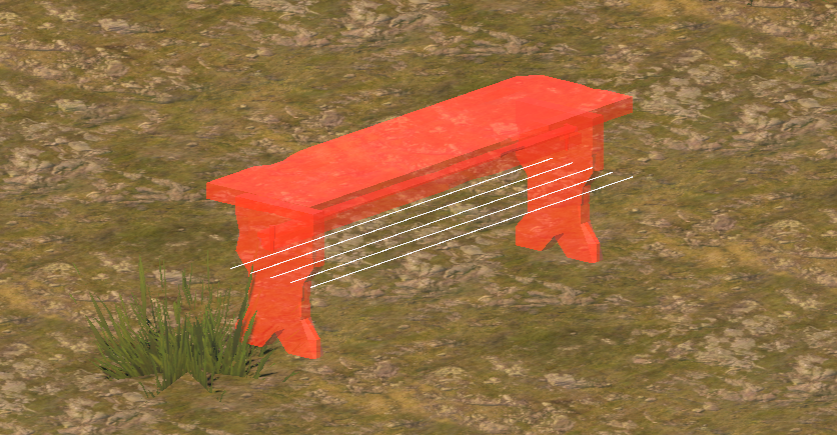
\includegraphics[width=1\textwidth]{images/implementacja/mechanizm_budowania/gizmos_drzewo_1.png}
   \caption{Widok z boku na siatkę promieni służących do wykrywania kolizji z drzewami.}
\end{figure}
\FloatBarrier

\section{Sterowanie jednostkami, podążanie za główną postacią (Zofia Sosińska)}\label{chap:sjpzgp}
Na samym początku gry stworzona przez gracza postać pojawia się sama. W tym momencie jest to jedyny obiekt, którym gracz może sterować.
Kontroluje, gdzie postać idzie, jak walczy oraz z kim rozmawia. Z biegiem czasu gra będzie jednak naciskać na formowanie drużyny,
ponieważ pokonywanie wielu przeciwników w pojedynkę będzie się stawało zbyt trudne. Pojawia się w takim momencie potrzeba 
zaimplementowania funkcjonalności zarządzania wieloma postaciami.

Stworzenie mechaniki poruszania się i oddziaływania na otaczający świat dla jednej postaci wydaje się proste i intuicyjne, ale kierowanie wieloma osobami już nie. 
Bez wprowadzenia zmian, używając jednego sposobu dyrygowania wszystkimi jednostkami tak samo, gra będzie prędko męczyć gracza.
Dla czynności małoznaczących, takich jak przemieszczenie drużyny w konkretne miejsce, wprowadzi monotonię i czasochłonność.
Każdą postać należy wybrać i przemieścić ją w konkretne miejsce. Kilka kliknięć przy jednej postaci jest akceptowalne, ale przy kilku wprowadzi to ogromne opóźnienia.

Jeszcze gorsze skutki pokazałyby się podczas walki. Szybkie przeskakiwanie pomiędzy postaciami podniosłoby zauważalnie trudność gry.
Poruszanie się jedną postacią i zabijanie przeciwników nie ma sensu, gdy reszta drużyny jest bita i nie może się obronić, ponieważ gracz musi się przełączyć na inną postać,
aby ta wykonała ruch. 

Z tego powodu potrzebny jest algorytm odpowiadający za właściwe poruszanie się pobocznych postaci.
Tworzona gra będzie dopuszczała małe, kilkunastoosobowe drużyny z przywódcą - postacią grywalną przez użytkownika - na czele.
Podczas walki graczowi pokażą się możliwe do wydania polecenia oraz specyfikacja, jakiej grupy mają one dotyczyć.
Za pomocą określonych klawiszy klawiatury będzie on mógł kontrolować zachowanie kompanów.

Po rozwiązaniu problemu mechaniki sterowania jednostkami w walce nie można przeoczyć samego poruszania się oraz interakcji ze światem.
Najprostszym rozwiązaniem będzie implementacja mechanizmu, według którego drużyna, po wykryciu znacznego przemieszczenia się przywódcy, sama będzie za nim podążać.
Kompani nie będą też mieli opcji samodzielnej interakcji ze światem, co sprawi, że poza walką zostaną jedynie biernymi obserwatorami.
\section{System dialogów. Bartosz Strzelecki}

System dialogów jest podstawową metodą, którą gracz będzie wykorzystywał, aby pozyskać informacje  o świecie oraz celach misji.
Gracz może inicjować konwersacje z postaciami niezależnymi, po czym zostaną mu zaproponowane opcje sposobu prowadzenia rozmowy.
W zależności od wybranych opcji dialogowych gracz może się spodziewać różnych konsekwencji.


\begin{figure}[h]
\centering
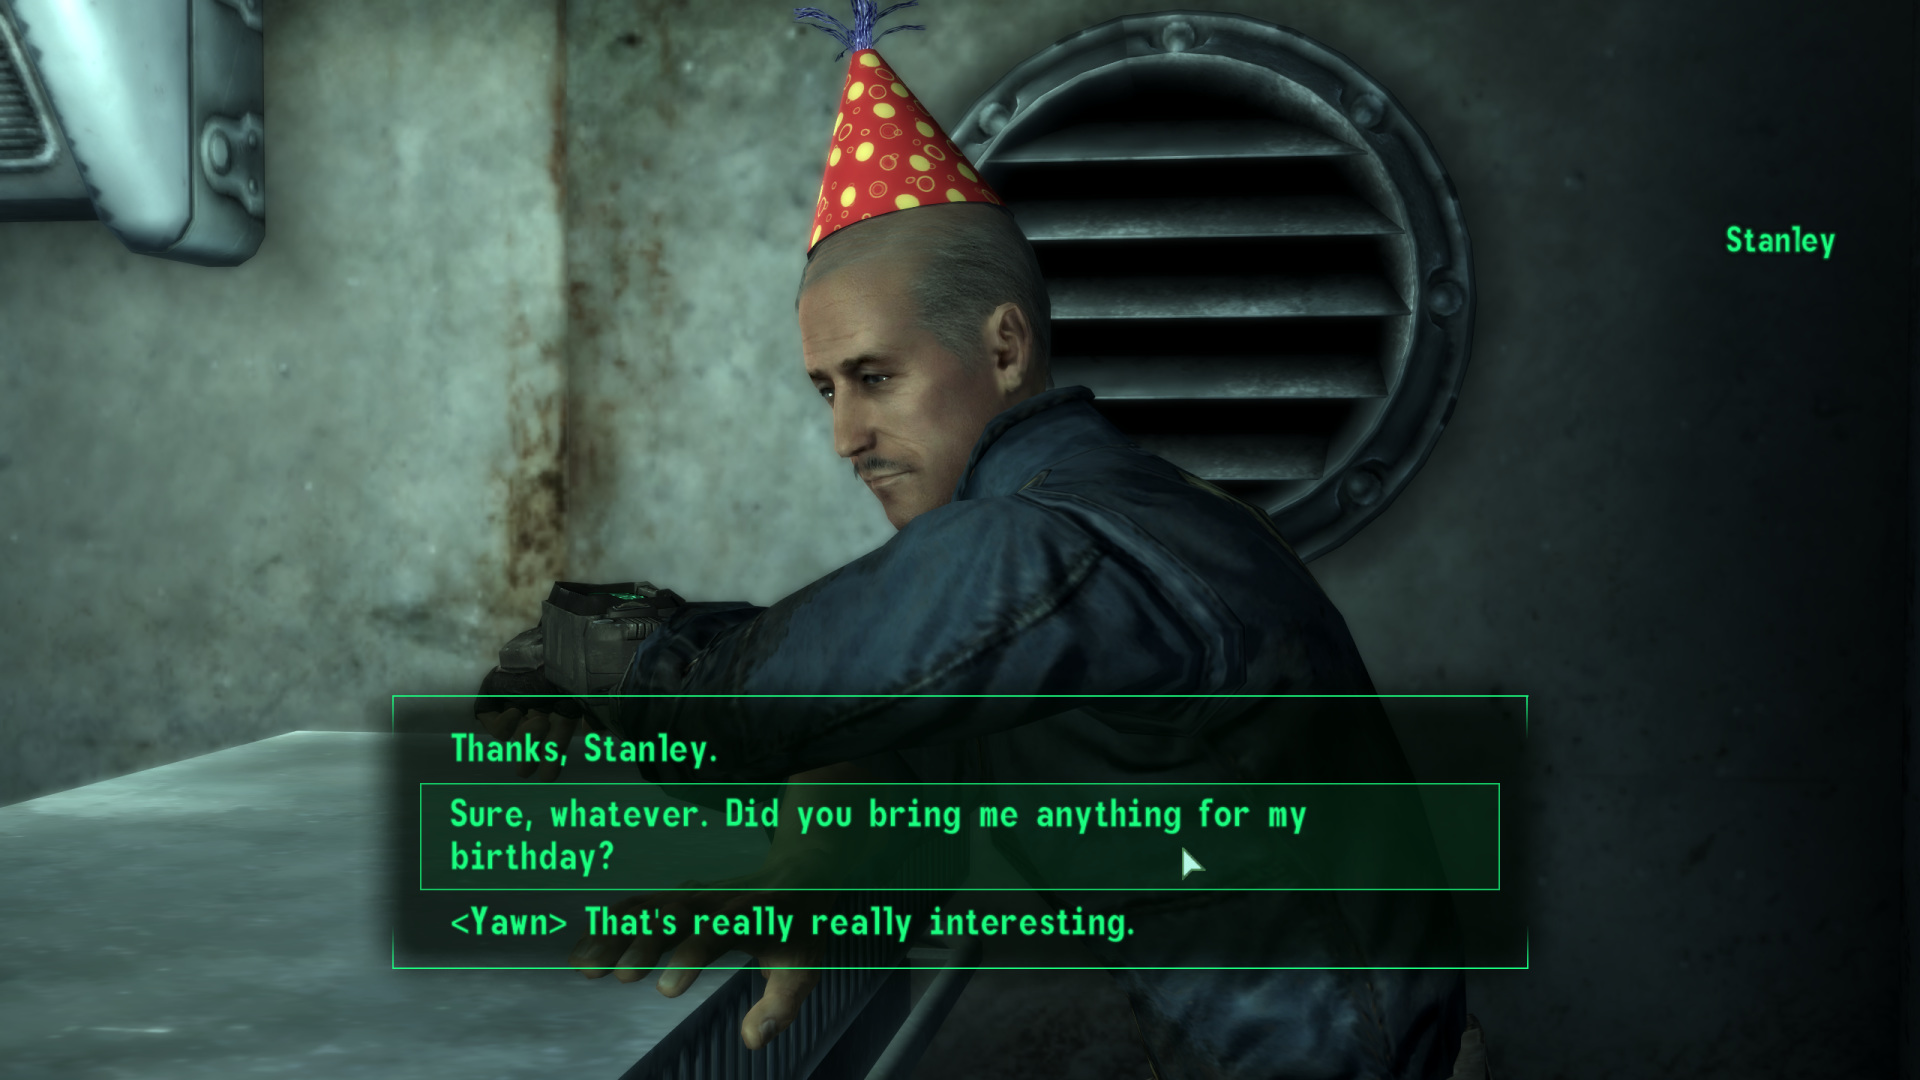
\includegraphics[width=0.6\textwidth]{images/fallout3}
\caption{Kadr z gry Fallout 3 przedstawiający przykładowy dialog}
\end{figure}

\href{https://assetstore.unity.com/packages/tools/utilities/dialogue-editor-168329}{Dialogue Editor} autorstwa Grasshop Dev jest prostym narzędziem pozwalającym na szybkie dodawanie i modyfikację dialogów.
Zawiera zestaw elementów ułatwiających wdrożenie systemu do projektu oraz udostępnia struktury danych wykorzystywanych do tworzenia interfejsu użytkownika.
Podczas rozmowy z postaciami niezależnymi gracz będzie mógł pozyskać informację o geografii świata, możliwych zagrożeniach oraz zadaniach do wykonania. 
Podobne systemy występują w grach takich jak Pillars of Eternity oraz w grach z serii Mass Effect.


\section{Sztuczna inteligencja (Bartosz Strzelecki)}\label{s:ai_impl}
Nawigacja przeciwników została zrealizowana poprzez wbudowany w silnik Unity system \texttt{NavMesh}. Pozwala on na łatwe wyznaczenie powierzchni, po której mogą poruszać
się postacie niekontrolowane przez gracza oraz realizuje zadanie wyznaczania ścieżki dla tych postaci.

\begin{figure}[h]
\centering
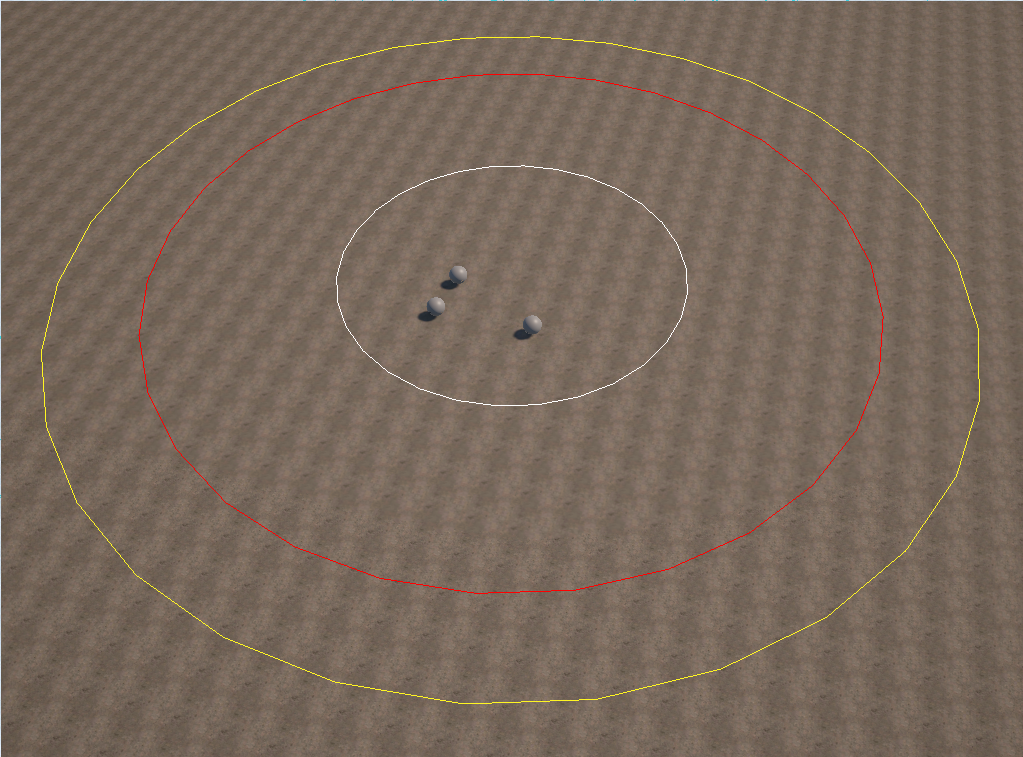
\includegraphics[width=0.9\textwidth]{images/ai}
\caption{Obraz przedstawia zasięgi odpowiednich regionów.}
\label{fig:regions}
\end{figure}
\FloatBarrier

Przeciwnicy są kontrolowani poprzez jeden obiekt przydzielający cele każdemu przypisanemu wrogowi. W normalnym trybie wrogowie poruszają się w sposób losowy
w obrębie wyznaczonej przestrzeni (biały okrąg na rys. \ref{fig:regions}). Kiedy przyjazne jednostki znajdą się w wystarczającej odległości (czerwony okrąg na rys. \ref{fig:regions}), przeciwnicy obiorą sobie za cel jedną z nich.
Po opuszczeniu przez drużynę gracza wyznaczonego obszaru (żółty okrąg na rys. \ref{fig:regions}) wrogowie wracają do poruszania się w sposób losowy w obrębie białego okręgu.


\begin{figure}[h]
\centering
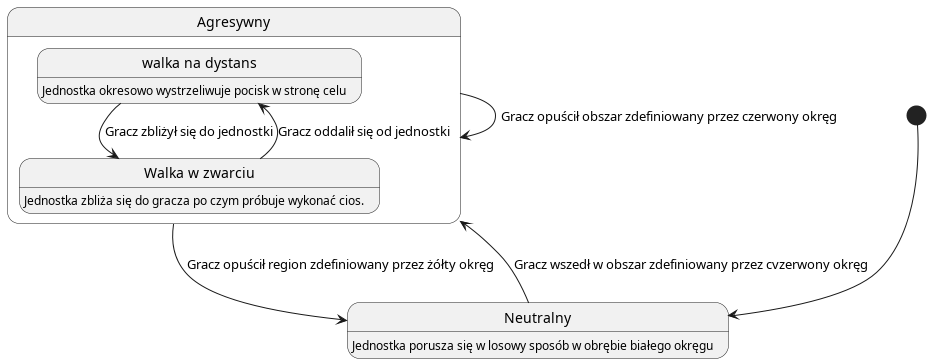
\includegraphics[width=1\textwidth]{uml/ai}
\caption{Diagram przedstawiający przepływ stanów dla sztucznej inteligencji przeciwników.}
\end{figure}
\FloatBarrier

\section{Widzenie przez horyzont (Bartosz Strzelecki)}\label{s:wid_impl}
Efekt został osiągnięty poprzez zmodyfikowanie potoku renderowania w taki sposób, że w zależności od wartości w buforze głębi jest wykorzystywany inny shader.
W tym przypadku, jeżeli sfera jest przysłonięta przez ścianę, jest ona narysowana, a w przeciwnym wypadku jest uruchamiany pusty shader.
"Unity domyślnie sortuje obiekty na podstawie odległości od kamery. Tak więc
w miarę zbliżania się obiektu do kamery, będzie on rysowany nad wszystkimi obiektami znajdującymi się dalej od kamery.
W większości przypadków sprawdza się to dobrze podczas tworzenia gier, ale
znajdą się sytuacje, w których będziemy chcieli mieć większą kontrolę nad sortowaniem obiektów na scenie. Używając bloku \verb|Tags\{\}| możemy kontrolować to sortowanie.
Unity udostępniło nam kilka domyślnych kolejek renderowania, z których każda ma unikalną wartość, którą
kieruje Unity, kiedy należy narysować obiekt na ekranie. Te wbudowane kolejki renderowania
nazywają się \verb|Background|, \verb|Geometry|, \verb|AlphaTest|, \verb|Transparent| i \verb|Overlay|." \cite{shaderscookbook}. Wykorzystując ten mechanizm
możliwe jest uzyskanie efektu widzenia przez postać gracza poprzez horyzont. Uzyskujemy przez to efekt podobny do tego zaimplementowanego w grze \textit{Dead by Daylight} (por. \ref{chap:dbd}).

Po naciśnięciu przycisku \texttt{E} następuje zagranie animacji opisanej wzorami

\begin{equation}
w(t, offset) = 1.1 \times 2.1^{-\left(\frac{{\left(\sin(t) + 1 - 0.4 - \text{{offset}}\right)^2}}{{0.02}}\right)}
\end{equation}

oraz

\begin{equation}
w(t, 0) - w(t, -0.2) + w(t, -1) - w(t, -1.2)
\end{equation}

Od podanych funkcji zależy przeźroczystość, jak i natężenie efektu Fresnela. 

\begin{figure}[h]
    \centering
    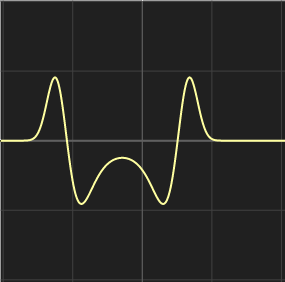
\includegraphics[width=0.5\textwidth]{images/g}
    \caption{Wykres przedstawiający funkcję opisującą natężenie efektu w animacji markera.}
\end{figure}



\begin{lstlisting}[language=C++, caption=Fragment shadera odpowiedzialny za animację.]
fixed4 frag (v2f i) : SV_Target
{
  float t =  6.2 * _Progress - 0.6;
  fixed4 pattern = tex2D(_PatternTex, i.uv + _Speed *t);
  float fresnelInfluence = dot(i.worldPos, i.viewDir);
  float saturatedFresnel = saturate(1 - fresnelInfluence);

  float g = w(t, 0) - w(t, -0.2) + w(t, -1) - w(t, -1.2);
  float4 color = pow(saturatedFresnel, g * _FresnelPow) * (_Color * _ColorIntensity) * pattern;
  color.a *= dot(i.worldPos, i.viewDir);
  return color;
}
\end{lstlisting}

\begin{figure}[h]
\centering
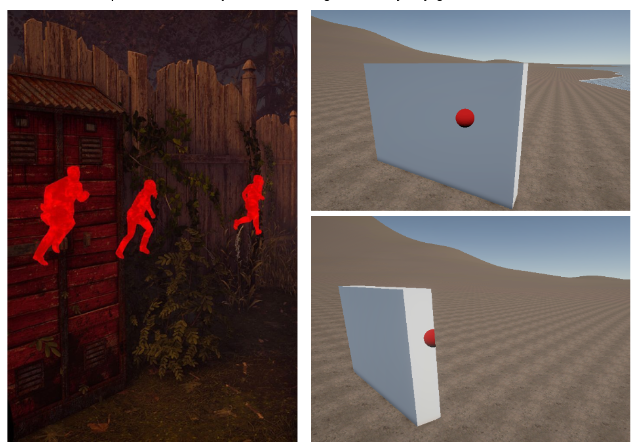
\includegraphics[width=0.6\textwidth]{images/shader}
\caption{Zachowanie programu cieniującego w przypadku przysłaniania markera przez przeszkody.}
\end{figure}

\chapter{Implementacja}
Ten rozdział skupia się na zaprezentowaniu implementacji projektu w silniku Unity.
Przedstawia on wykorzystane metodyki i narzędzia wykorzystane do osiągnięcia określonych wymagań.
Jak również zawiera fragmenty wykorzystanych algorytmów i zrzuty ekranu reprezentujące efekty pracy.

\section{Kontroler postaci. Bogna Lew}

W trakcie rozgrywki istotnym aspektem wpływającym na jakość jest mechanizm sterowania postacią. Z tą mechaniką gracz ma
bezpośredni kontakt, ponieważ to właśnie za jej pomocą może eksplorować świat.

Do implementacji tego mechanizmu zainspirowaliśmy się grą Skyrim. Postać jest sterowana za pomocą klawiszy “w”, “a”, “s”
oraz “d”, natomiast jej rotacja oraz obrót kamery jest kontrolowany przez mysz. Całość została podzielona na cztery
części.

Pierwsza z nich odpowiada za przemieszczanie się postaci. Do tego wykorzystuje Input Manager, w którym zostały
zmapowane odpowiednie klawisze dla każdej z osi, wzdłuż której gracz może się przemieszczać. W rezultacie powstały dwa
kierunki - przód/tył oraz prawo/lewo. Naciśnięcie odpowiedniego przycisku skutkuje zwróceniem wartości 1 bądź -1, które
symbolizują zwrot wektora przemieszczenia wzdłuż osi. Na tej podstawie wyznaczane jest faktyczne przesunięcie postaci
względem kierunku, w którym jest zwrócona oraz modyfikowane jest jej położenie. Dodatkowo ten komponent odpowiada za
wyznaczenie prędkości, z jaką gracz się porusza. Domyślnie postać przemieszcza się tempem chodu, jednakże jeśli gracz
przytrzyma lewy klawisz Shift, to zacznie się poruszać biegiem.

Druga część kontrolera odpowiada za ustawienie odpowiedniej animacji. Do tego wykorzystuje ona wartości zwrotu wzdłuż
obu osi oraz prędkość, które są wyznaczane w poprzednim komponencie. Na ich podstawie wyznacza kolejne części nazwy
animacji, po czym, jeśli jest inna niż aktualnie wyświetlana, uruchamia ją.

Kolejny komponent nadzoruje rotację postaci oraz co za tym idzie - kamery. Analogicznie wykorzystywany jest Input
Manager, jednak w tym przypadku przechwytywane jest przesunięcie myszy. Komponent udostępnia graczowi możliwość
sterowania kierunkiem, w którym postać patrzy, a co za tym idzie - względem którego się przemieszcza. Jednocześnie
następuje dostosowanie położenia kamery tak, aby zawsze patrzyła w tym samym kierunku co postać gracza. Ponadto
komponent umożliwia przesunięcie kamery po łuku do góry bądź do dołu. Dzięki temu gracz może dokładniej zobaczyć
co znajduje się nad oraz tuż przed nim.

Ostatni komponent odpowiada za kontrolowanie przybliżania kamery. W tym celu w Input Managerze zostało zamapowane kółko
myszy. Zwrócona przez system wartość jest wykorzystywana do obliczenia odległości kamery od postaci przy zachowaniu
ustalonych przez grę ograniczeń. Dodatkowo, komponent dokonuje również automatycznego przybliżania, jeśli wskutek
przemieszczania się postaci, pomiędzy nią, a kamerą miałaby się znaleźć przeszkoda. Dzięki temu nie zostanie zasłonięty
widok tego co się dzieje wokół postaci. Odsunięcie się od przeszkody zaskutkuje oddaleniem kamery do poprzedniej
odległości.

\section{Interfejs Użytkownika (Zofia Sosińska)}\label{chap:ui_imp}
Interfejs użytkownika, jako uporządkowany i przejrzysty obraz wiedzy i możliwych opcji granej postaci odciąża użytkownika
aplikacji, zdejmując z niego przymus pamiętania dokładnie każdej pojawiającej się informacji. Umililiśmy i uprościliśmy 
rozgrywkę, przedstawiając suche dane w postaci przyjemnych dla oka obrazów, wyszczególniając to, co jest najważniejsze.

Tak jak przewidywano, UI udostępnia interfejs podstawowy z zawsze widocznymi elementami oraz dynamicznie pojawiające się okna, wywoływane za pomocą konkretnych klawiszy.
Wszystkie łączy surowy i prosty przewodni motyw graficzny, wykorzystujący także różnorodne obrazy dla urozmaicenia. Przy implementacji ważne także było, aby UI zabierał
jak najmniej miejsca, jednocześnie podając jak najwięcej przydatnych informacji.

\subsection{Interfejs podstawowy}
Interfejs podstawowy towarzyszy graczowi podczas całej rozgrywki. Skupia się on w górnej części ekranu. Jego zadaniem jest pomoc 
użytkownikowi w ogólnym odnalezieniu się w świecie. W tym celu są mu ukazane następujące informacje:
\begin{itemize}
    \item aktualny czas w grze;
    \item położenie gracza względem stron świata oraz wrogów ukazane na kompasie;
    \item stan surowców i funduszy;
    \item stan zdrowia gracza;
    \item etap, na którym są przypisane graczowi zadania.
\end{itemize}

\begin{figure}[htbp]
    \centering
    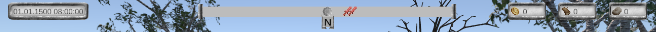
\includegraphics[width=0.9\textwidth]{images/ui/naszpasek.png}
    \caption{Implementacja paska z najważniejszymi informacjami o stanie gry: aktualnym czasie, posiadanych surowcach 
    i funduszach, położeniu i otoczeniu gracza, zdrowiu postaci oraz ikona sygnalizująca, czy użytkownik ma do wykonania jakieś zadanie.
    }\label{fig:naszpasek}
\end{figure}

W tych statycznie umiejscowionych elementach interfejsu dynamicznie zmienia się ich treść. Na zegarze czas zmienia się w ustalony sposób,
dodając minutę w grze co 5 sekund upływające w realnym świecie. Na kompasie umiejscowienie zmieniają symbole stron świata i wskaźniki przeciwników,
zależnie od ich pozycji, położenia gracza i strony, w którą główna postać patrzy. Fundusze rosną po wykonaniu zadania i otrzymaniu zapłaty oraz maleją, gdy opłacamy
najemników, czy płacimy za budowle. Liczba posiadanych surowców zwiększa się, po zebraniu ich z ziemi, za to zmniejsza, gdy za ich pomocą budujemy budynek.  
Pasek zdrowia zmienia swoją wartość, gdy dostaniemy obrażenia, jednocześnie ukazując początkową, maksymalną wartość. Ikona zadania do wykonania ukazuje symbol 
czerwonego wykrzyknika, gdy gracz ma jakieś aktywne, nieskończone zadanie, co ukazano na rysunku \ref{fig:wyq}.
\begin{figure}[htbp]
    \centering
    
\includegraphics[width=0.5\textwidth]{images/ui/wykrzyknik_quest.png}
    \caption{Implementacja ikony zadania do wykonania, gdy użytkownik ma jakieś nieskończone zlecenia.
    }\label{fig:wyq}
\end{figure}

\subsection{Menu stawiania budynków}
Typowa mechanika gier typu RTS, czyli budowanie budynków, ma specjalnie przygotowany interfejs, wyświetlany po wciśnięciu klawisza "B". 
Ulokowany on został w dolnej części ekranu. Najważniejszym elementem menu stawiania budynków jest lista dostępnych budowli. Widnieją tam 
obrazy ukazujące każdą z nich, a gracz ma wgląd w ich szczegóły poprzez zmianę aktywnej prawą i lewą strzałką. Wtedy wokół niej pokazują się także informacje dotyczące jej kupna,
a po lewej stronie ekranu - informacja o ewentualnym nieprawidłowym umiejscowieniu. W wypadku, gdy zakup jest niemożliwy z powodu niewystarczającej liczby 
surowców, pojawi się stosowny komunikat. Menu zamyka się za pomocą klawisza "Escape".
\begin{figure}[htbp]
    \centering
    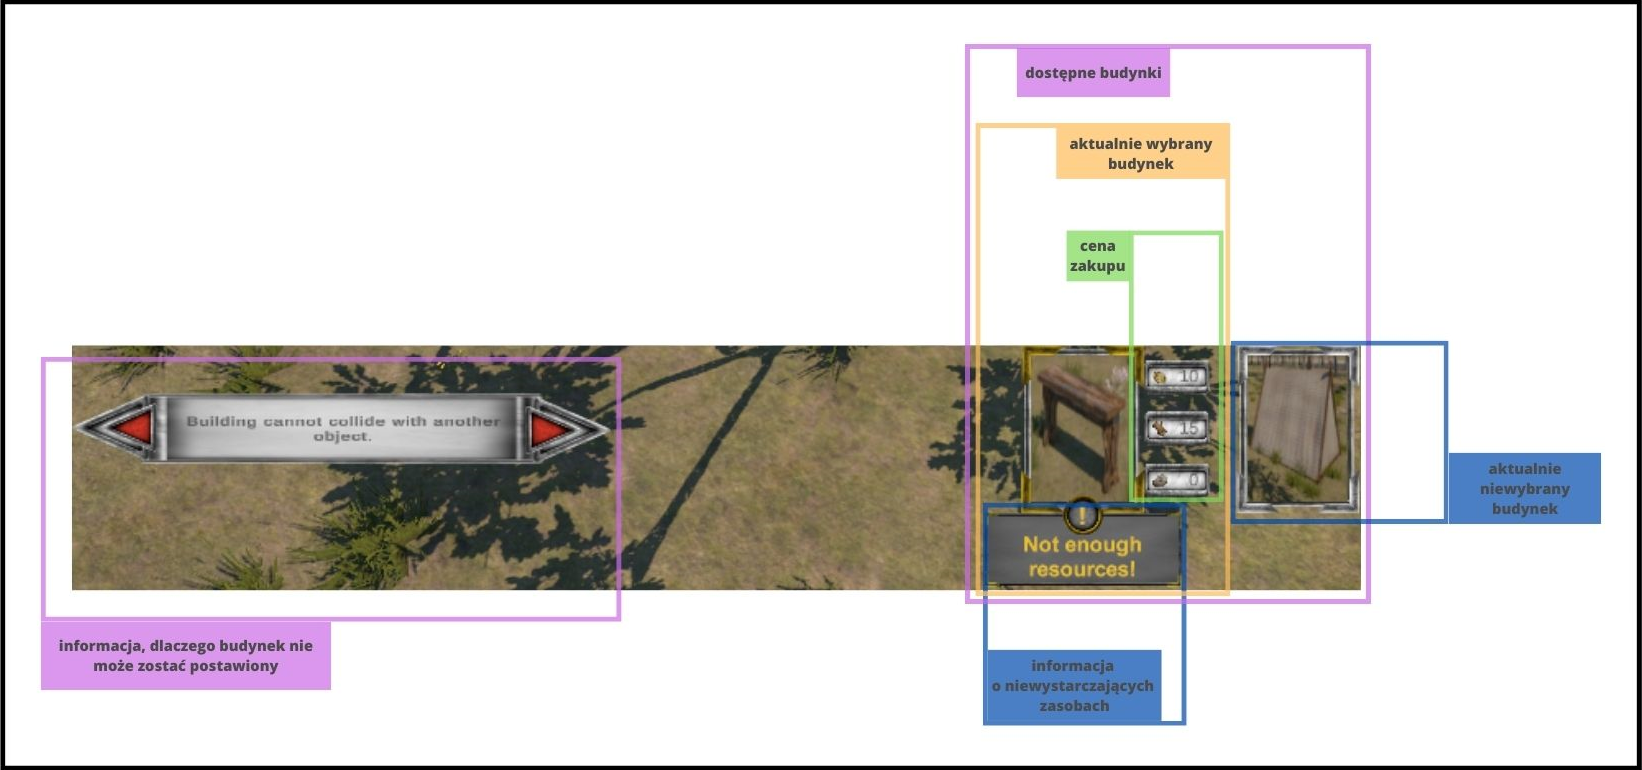
\includegraphics[width=0.9\textwidth]{images/ui/opis_ekementow_budowanie.png}
    \caption{Implementacja menu stawiania budynków, na którym pokazane są możliwe do zbudowania budowle 
    i szczegółowe informacje o ich dostępności.
    }\label{fig:compass}
\end{figure}

\subsection{Menu wydawania komend}
Gra umożliwia graczowi wykupienie usług najemników, jeśli dysponuje odpowiednimi funduszami. Gdy są oni już pod dowództwem użytkownika, może on im rozkazywać za pomocą 
menu wydawania komend. Po naciśnięciu klawisza "Q" pokazuje się lista dostępnych grup podwładnych, podzielonych według ich specjalizacji. Po wybraniu jednej z nich 
wylistowane zostaną możliwe do rozkazania czynności. W obu przypadkach gracz ma także możliwość anulowania. 
\begin{figure}[htbp]
    \centering
    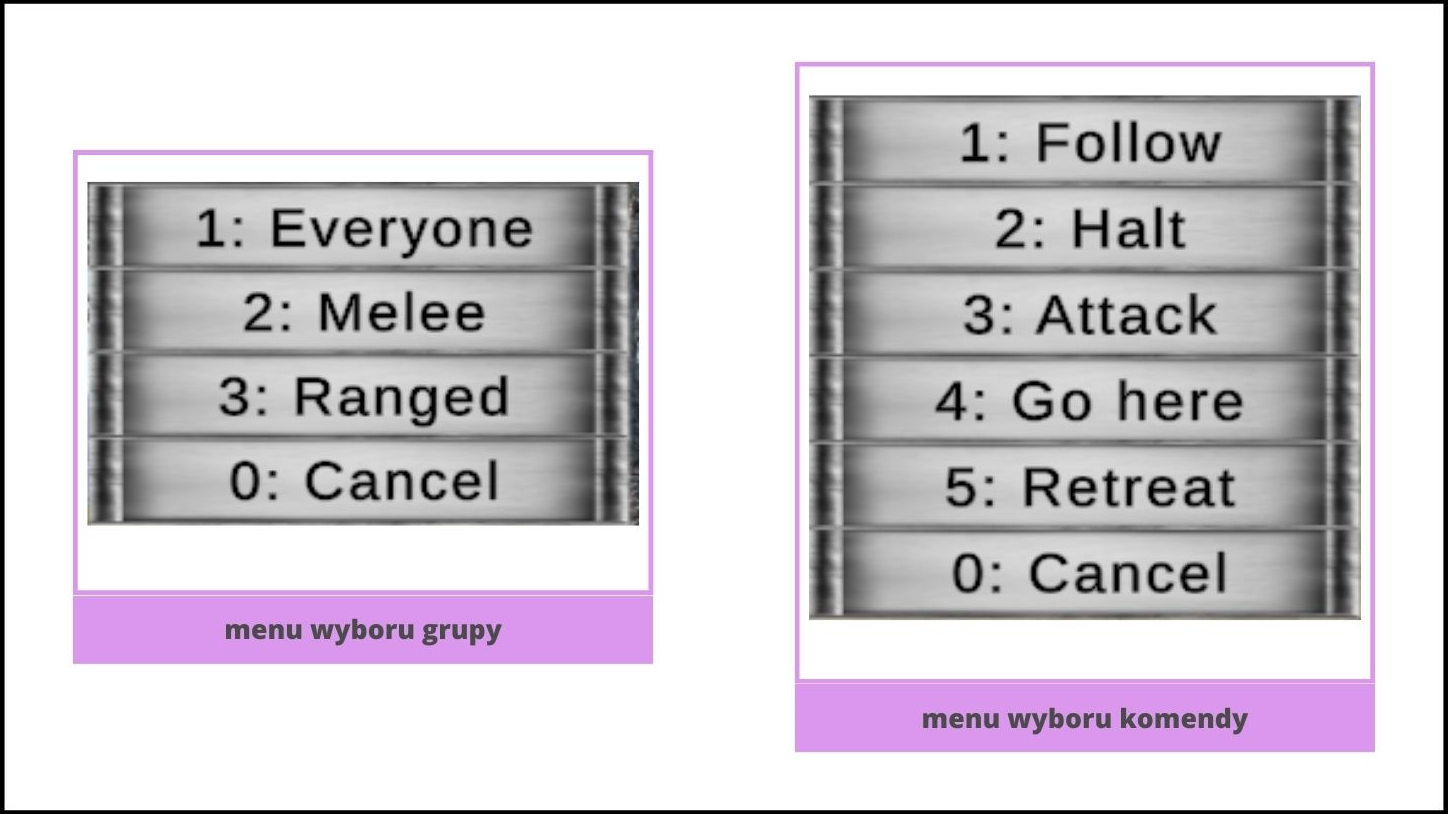
\includegraphics[width=0.9\textwidth]{images/ui/opis_ekementow_mwnu_wyboru_komendy.png}
    \caption{Implementacja menu wydawania komend.}\label{fig:cmd_menu}
\end{figure}

\subsection{Menu zapisu}
Po uznaniu przez gracza, że nie chce stracić aktualnego stanu gry, może go permamentnie zapisać w pamięci urządzenia, na którym włączony jest program. Po naciśnięciu 
klawisza "Z" pojawia sie menu zapisu. Gracz może odczytać z niego nazwę pliku, w którym zapisany zostanie stan gry. W menu znajduje się także informacja o tym, że 
poprzez ponowne naciśnięcie klawisza "Z" potwierdzi on zapis. 
\begin{figure}[htbp]
    \centering
    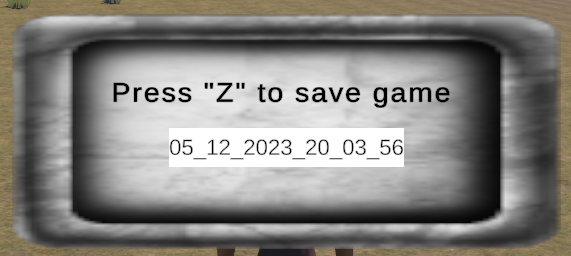
\includegraphics[width=0.9\textwidth]{images/ui/menu_zapisu.png}
    \caption{Implementacja menu zapisu.}\label{fig:men_zap}
\end{figure}

\subsection{Informacja o możliwej interakcji}
W świecie gry postać gracza nie jest odosobniona, co więcej może spotkać wiele różnorodnych osób, z którymi można porozmaiwać. Interaktywni
jednak nie są tylko ludzie, ale i surowce, które można zbierać. Jeśli możliwa jest interakcja,  wyświetlana jest informacja o takim stanie
 rzeczy. Zaraz pod kompasem pojawia się grafika instruująca, że po naciśnięciu klawisza "E" klawiatury, postać gracza wykona opisaną czynność.
 \begin{figure}[htbp]
    \centering
    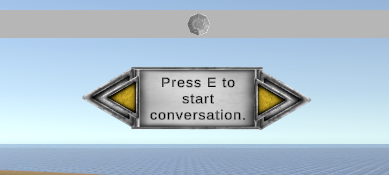
\includegraphics[width=0.9\textwidth]{images/ui/interakcja_rozmowa.png}
    \caption{Implementacja grafiki informującej o możliwości rozpoczęcia rozmowy.}\label{fig:rozmow}
\end{figure}
\begin{figure}[htbp]
    \centering
    \includegraphics[width=0.9\textwidth]{images/ui/interakcja_podnieś.png}
    \caption{Implementacja grafiki informującej o możliwości podniesienia przedmiotu.}\label{fig:przedmio}
\end{figure}

\subsection{Dziennik z zadaniami}
Niektóre postacie interaktywne mogą zlecić głównemu bohaterowi zadanie. Jeśli gracz się zgodzi, notatka o nim zostaje zapisana w dzienniku. Można do niego zajrzeć
wciskając klawisz "J". Graczowi ukaże się tytuł sygnalizujący główny cel zadania, streszczenie najważniejszych informacji oraz porada dotycząca mechanik gry np. 
"Wciśnij klawisz X, żeby stało się Y". To, że zadanie nie zostało jeszcze wykonane, sygnalizuje czerwony wykrzyknik w prawym, górnym rogu notatki. Gracz może 
zamknąć dziennik poprzez ponowne naciśnięcie klawisza "J".
\begin{figure}[htbp]
    \centering
    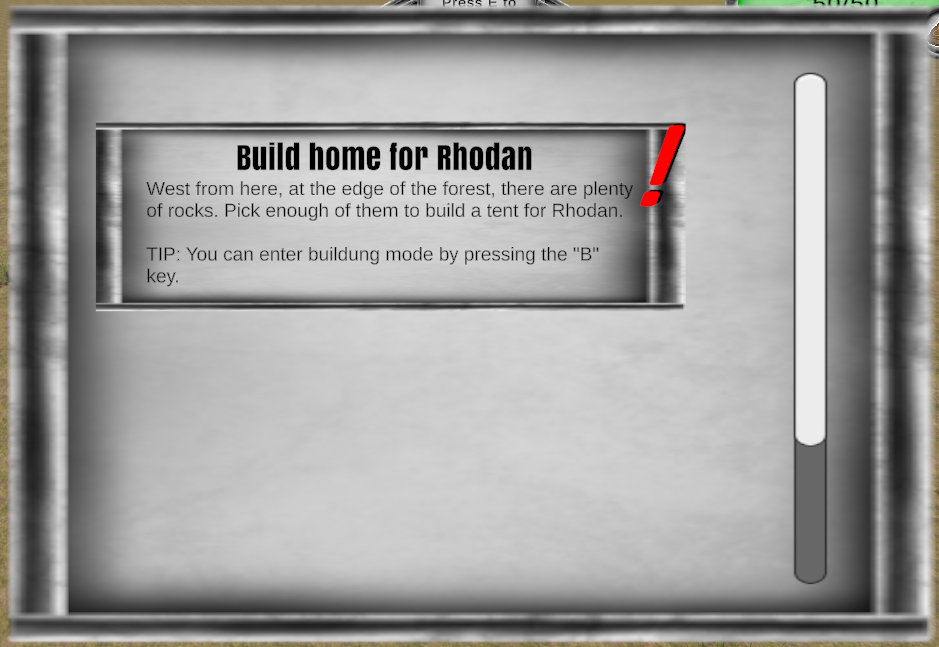
\includegraphics[width=0.9\textwidth]{images/ui/journal_quest.png}
    \caption{Implementacja dziennika z aktualnie zaczętym i nieukończonym zadaniem.}\label{fig:end_sc}
\end{figure}

\subsection{Ekran końca gry}
Postać gracza ma określoną liczbę punktów życia, które może stracić podczas potyczek z przeciwnikami. Gdy spadną one do zera gra kończy się, a główny bohater umiera.
W takim wypadku graczowi pojawia się ekran końca gry, który informuje go o śmierci oraz o możliwości przejścia do menu głównego. Aby jeszcze bardziej uwypuklić zakończenie 
rozgrywki, cały ekran zostaje przyciemniony.
\begin{figure}[htbp]
    \centering
    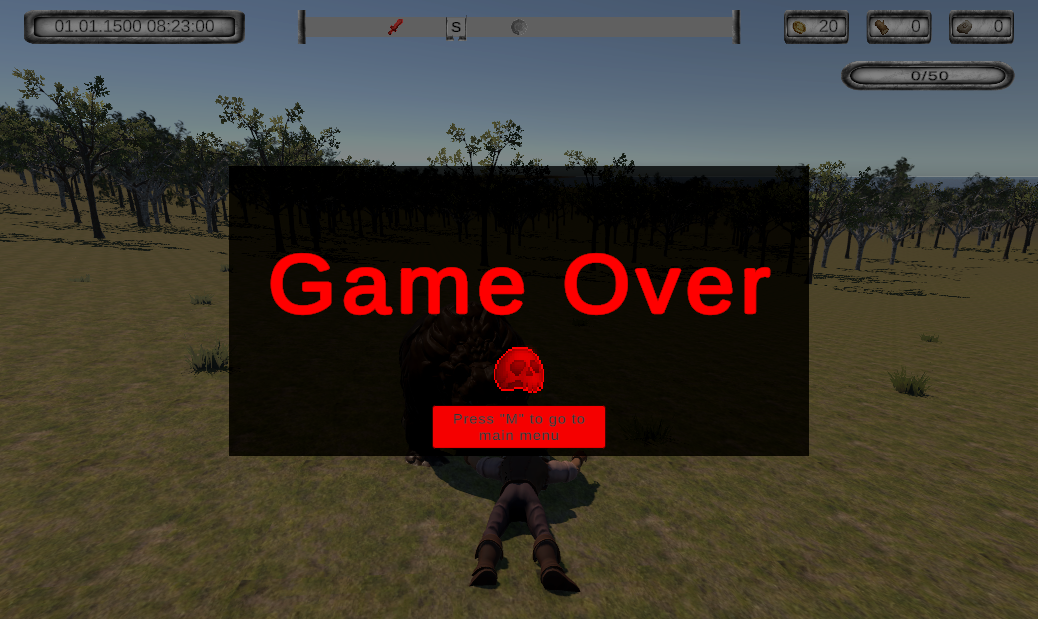
\includegraphics[width=0.9\textwidth]{images/ui/endgame_screen.png}
    \caption{Implementacja menu zapisu.}\label{fig:end_sc}
\end{figure}

\section{Zasady działania kompasu (Zofia Sosińska)}\label{chap:naw_impl}

Projekt kompasu jest na tyle prosty, aby nie przytłoczyć gracza nadmierną liczbą bodźców. Składa się z horyzontalnego, jednolitego paska,
 na którym wyświetlane są najważniejsze informacje o otoczeniu, symbol ośmiokąta, wskazujący na przestrzeń znajdującą się centralnie przed bohaterem
  oraz z bocznych pasków, wyróżniających końce narzędzia.

\begin{figure}[htbp]
    \centering
    \includegraphics[width=0.9\textwidth]{images/ui/opis_ekementow_kompasu.png}
    \caption{Rozpiska elementów: a. główny pasek, b. symbol środka, c1., c2. paski końców kompasu.}\label{fig:compass_design}
\end{figure}
\FloatBarrier
Ikony wyświetlane na kompasie przedstawiają najważniejsze informacje w polu widzenia gracza, czyli stronę świata, w kierunku której jest on zwrócony, oraz przeciwników.
Poniżej przedstawiono kod odpowiedzialny za wyznaczenie pozycji symbolu na omawianym narzędziu. Wejściem jest komponent \texttt{RectTransform} symbolu przypisanego
danemu obiektowi oraz jego położenie. Po obliczeniu wektora prowadzącego do uzyskania np. pozycji wroga, wyznaczany jest kąt, o jaki musi się obrócić.
To jest przeliczane na pozycję na kompasie i jeśli obiekt znajduje się w polu widzenia postaci gracza to jest wyświetlany odpowiedni symbol.

\begin{figure}[htbp]
    \centering
    \includegraphics[width=0.9\textwidth]{images/ui/compass.png}
    \caption{Wizualizacja przypadku, w którym gracz patrzy centralnie na obozowisko wrogów. Na przeciwko oraz po lewej stronie znajdują się przeciwnicy, co jest zasygnalizowane na kompasie za pomocą symboli mieczy. Znajduje się na nim także informacja, że bohater jest lekko odchylony od Zachodu.
    }\label{fig:compass}
\end{figure}
\FloatBarrier
    \begin{lstlisting}[language=C++, caption=Fragment kodu odpowiedzialny za ustawienie symbolu na pasku kompasu.]
    void SetMarkerPosition(RectTransform markerTransform, Vector3 worldPosition)
    {
        Vector3 dirToTarget = worldPosition - CameraTransform.position;
        float angle = Vector2.SignedAngle(new Vector2(dirToTarget.x, dirToTarget.z), 
                                            new Vector2(CameraTransform.transform.forward.x, CameraTransform.transform.forward.z));
        float compassPositionX = Mathf.Clamp(
                                            2 * angle / Camera.main.fieldOfView, -1, 1);
        if (compassPositionX == 1 || compassPositionX == (-1))
        {
            markerTransform.anchoredPosition = new Vector2(0, 100);
        }
        else
        {
            markerTransform.anchoredPosition = new Vector2(
                compassBarTransform.rect.width / 2 * compassPositionX, 0);
        }
    }
    \end{lstlisting}
\FloatBarrier
Problem lokalizacji stron świata pojawił się, gdy nieprawidłowo wyświetlały się symbole po użyciu najprostszego rozwiązania. Na przykład dla Północy było to
pobranie wartości od \texttt{Vector3.forward}, co jest skrótowym zapisem \texttt{Vector3(0, 0, 1)}. Lewy dolny róg mapy jest położony w punkcie (0, 0, 0), co oznacza, że wymagane
jest przesunięcie, aby prawidłowo zasymulować strony świata. Północ i Południe  zostały przesunięte do połowy szerokości, a Wschód i Zachód - długości mapy. Każde z nich
zostało oddalone o 60000 jednostek, co pozwala na wiarygodną symulację stron świata na kompasie.

\begin{figure}[htbp]
    \centering
    \includegraphics[width=0.9\textwidth]{images/ui/strony_swiata.png}
    \caption{Rozmieszczenie zasymulowanych stron świata.}\label{fig:world_sides}
\end{figure}
\FloatBarrier
Wykrycie wrogich jednostek znajduje się w funkcji Start. Każdemu obiektowi jest przypisywany symbol czerwonego miecza i w zależności od położenia wroga, obrazek wyświetlany jest odpowiednio na kompasie.
\begin{lstlisting}[language=C++, caption=Fragment kodu odpowiedzialny za połączenie wrogich obiektów na mapie z symbolami wyświetlonymi na kompasie.]
    void SetPositionOfEnemies()
    {
        foreach (
            var e in enemiesOnMap.Zip(enemiesOnUI, (x, y) => new {enemyOnMap = x, 
                                                                    enemyOnUI = y }))
        {
            SetMarkerPosition(e.enemyOnUI.GetComponent<RectTransform>(), 
                                e.enemyOnMap.transform.position);
        }
    }
\end{lstlisting}

\section{Mechanizm budowania (Bogna Lew)}\label{s:bud_impl}

Opracowany mechanizm umożliwia graczowi na przełączenie się w tryb budowania poprzez naciśnięcie klawisza \texttt{B}, który od razu
wyświetli podgląd bazowego obiektu. Widok budynku przemieszcza się przed postacią oraz odpowiednio obraca się razem z
nią. Efekt poruszania się podglądu został uzyskany za pomocą poniższego wzoru:
\begin{equation}
\begin{cases}
x = r \times sin(\alpha) \\
y = 0 \\
z = r \times cos(\alpha)
\end{cases}
\end{equation}

gdzie $x$, $y$ i $z$ to współrzędne odpowiednio względem osi X, Y i Z, $r$ to odległość środka obiektu od postaci
gracza, natomiast $\alpha$ to kąt o jaki jest on obrócony względem osi Y.

Podgląd budynku będzie widoczny do czasu, aż gracz go umieści naciskając prawy przycisk myszy bądź wychodząc z trybu
edycji naciskając klawisz \texttt{Escape}. Jeżeli widok budowli znajduje się w poprawnym do umieszczenia miejscu to jest on
podświetlany na zielono, w przeciwnym razie - na czerwono. Wybudowanie powoduje przywrócenie bazowych kolorów obiektu
oraz włącza wykrywanie kolizji z nim, dzięki czemu budynek poprawnie oddziałuje z otaczającym go środowiskiem.

\begin{figure}[h!]
    \centering
    \includegraphics[width=1\textwidth]{images/implementacja/mechanizm_budowania/poprawne.png}
    \caption{Przykład podglądu w poprawnym umiejscowieniu.}
\end{figure}
\FloatBarrier

Do weryfikacji poprawności umiejscowienia budynku wykorzystano mechanizmy wyzwalacza (ang. \textit{trigger}) oraz rzucania
promienia (ang. \textit{raycasting}). Pierwszy z nich polega na wykrywaniu czy obiekt znalazł się w obszarze kolizji bez
brutalnego zatrzymywania go. Oznacza to, że może on przeniknąć przez inny element bez widocznych konsekwencji, jedynie
wysyłając sygnał, że dana sytuacja nastąpiła. Druga metoda natomiast polega na wypuszczeniu promienia o pewnej długości
w zadanym kierunku i sprawdzeniu, czy z czymś się zderzył.

Wyzwalacz został zastosowany do wykrywania kolizji z innymi obiektami na mapie, takimi jak postacie, czy elementy
scenerii niebędące terenem. W tym celu wykorzystano metody \verb|OnTriggerEnter()| i \verb|OnTriggerExit()|, które są wywoływane
odpowiednio gdy, dany obiekt znalazł się w obszarze kolizji innego elementu, bądź go opuścił. Każda z nich odpowiednio
zmienia poprzez zwiększenie bądź zmniejszenie wartości licznika kolizji obiektu. Jeżeli jego wartość jest różna od zera, tzn.
obiekt z czymś koliduje, to umiejscowienie jest uznawane za niepoprawne.

Drugi z mechanizmów został wykorzystany do sprawdzenia nachylenia podłoża. Efekt został osiągnięty poprzez rzucenie
promienia o niewielkiej długości z każdego z dolnych narożników obiektu i zliczeniu ile z nich wykryło kolizję z ziemią.
Brak wykrycia kolizji można zinterpretować jako zapadanie się bądź zbyt mocne lewitowanie danego narożnika nad
powierzchnią ziemi. Z tego powodu przyjęto, że jeśli co najmniej trzy z nich zderzyły się z podłożem, to umiejscowienie
jest poprawne.

\begin{figure}[h!]
    \centering
    \includegraphics[width=1\textwidth]{images/implementacja/mechanizm_budowania/niepoprawne.png}
    \caption{Przykład podglądu w niepoprawnym umiejscowieniu.}
\end{figure}
\FloatBarrier

Dodatkowo metodę rzucania promienia wykorzystano do wykrycia kolizji z drzewami. Obiekty te są traktowane przez silnik
jako część terenu, przez co metoda wykorzystująca wyzwalacz pomija je. Dlatego w celu wykrywania kolizji z nimi
zdecydowano się na rzucenie dwóch grup promieni biegnących w głąb obiektu z naprzeciwległych krawędzi prostopadłych do
osi Y. Każdy z promieni biegnie w połowie wysokości obiektu i sięga przeciwnej ściany. Tak skomplikowany układ ma na
celu zapewnienie poprawności wykrywania kolizji w przypadku, gdy początki promieni znajdują się wewnątrz kolidującego
obiektu. Jeśli którykolwiek z nich zderzy się z drzewem, to wybrane miejsce jest uznawane za niepoprawne.

\begin{figure}[h!]
   \centering
   \includegraphics[width=1\textwidth]{images/implementacja/mechanizm_budowania/gizmos_drzewo_2.png}
   \caption{Widok z góry na siatkę promieni służących do wykrywania kolizji z drzewami.}
\end{figure}
\FloatBarrier
\begin{figure}[h!]
   \centering
   \includegraphics[width=1\textwidth]{images/implementacja/mechanizm_budowania/gizmos_drzewo_1.png}
   \caption{Widok z boku na siatkę promieni służących do wykrywania kolizji z drzewami.}
\end{figure}
\FloatBarrier

\section{System dialogów. Bartosz Strzelecki}

System dialogów jest podstawową metodą, którą gracz będzie wykorzystywał, aby pozyskać informacje  o świecie oraz celach misji.
Gracz może inicjować konwersacje z postaciami niezależnymi, po czym zostaną mu zaproponowane opcje sposobu prowadzenia rozmowy.
W zależności od wybranych opcji dialogowych gracz może się spodziewać różnych konsekwencji.


\begin{figure}[h]
\centering
\includegraphics[width=0.6\textwidth]{images/fallout3}
\caption{Kadr z gry Fallout 3 przedstawiający przykładowy dialog}
\end{figure}

\href{https://assetstore.unity.com/packages/tools/utilities/dialogue-editor-168329}{Dialogue Editor} autorstwa Grasshop Dev jest prostym narzędziem pozwalającym na szybkie dodawanie i modyfikację dialogów.
Zawiera zestaw elementów ułatwiających wdrożenie systemu do projektu oraz udostępnia struktury danych wykorzystywanych do tworzenia interfejsu użytkownika.
Podczas rozmowy z postaciami niezależnymi gracz będzie mógł pozyskać informację o geografii świata, możliwych zagrożeniach oraz zadaniach do wykonania. 
Podobne systemy występują w grach takich jak Pillars of Eternity oraz w grach z serii Mass Effect.


\section{Sztuczna inteligencja (Bartosz Strzelecki)}\label{s:ai_impl}
Nawigacja przeciwników została zrealizowana poprzez wbudowany w silnik Unity system \texttt{NavMesh}. Pozwala on na łatwe wyznaczenie powierzchni, po której mogą poruszać
się postacie niekontrolowane przez gracza oraz realizuje zadanie wyznaczania ścieżki dla tych postaci.

\begin{figure}[h]
\centering
\includegraphics[width=0.9\textwidth]{images/ai}
\caption{Obraz przedstawia zasięgi odpowiednich regionów.}
\label{fig:regions}
\end{figure}
\FloatBarrier

Przeciwnicy są kontrolowani poprzez jeden obiekt przydzielający cele każdemu przypisanemu wrogowi. W normalnym trybie wrogowie poruszają się w sposób losowy
w obrębie wyznaczonej przestrzeni (biały okrąg na rys. \ref{fig:regions}). Kiedy przyjazne jednostki znajdą się w wystarczającej odległości (czerwony okrąg na rys. \ref{fig:regions}), przeciwnicy obiorą sobie za cel jedną z nich.
Po opuszczeniu przez drużynę gracza wyznaczonego obszaru (żółty okrąg na rys. \ref{fig:regions}) wrogowie wracają do poruszania się w sposób losowy w obrębie białego okręgu.


\begin{figure}[h]
\centering
\includegraphics[width=1\textwidth]{uml/ai}
\caption{Diagram przedstawiający przepływ stanów dla sztucznej inteligencji przeciwników.}
\end{figure}
\FloatBarrier

\subsection{Mechanika zachowań klas jednostek}
\subsubsection{Jednostki walczące w zwarciu}
Zachowanie jednostek bliskiego zasięgu polega na wybraniu przeciwnika będącego w czerwonym obszarze (rys. \ref{fig:regions}), który ma najwyższą
wartość priorytetu obliczonego między innymi na podstawie odległości, ilości innych atakujących przeciwników oraz klasy celu.
Jednostka posiadająca cel ataku zmierza w jego kierunku, obierając najkrótszą drogę. Po dotarciu do celu podróży jednostki biorące udział w walce
losują naprzemiennie liczby, od których zależy wynik walki, jak i aktualnie wykorzystywana animacja.

\subsubsection{Jednostki walczące na dystans}
Takie jednostki wystrzeliwują w stronę przeciwników pociski, których celność jest reprezentowana przez dwie strefy (rys. \ref{fig:acc2}). Jedną oznaczającą 50\% celności,
czyli rozrzut, który będzie posiadała połowa pocisków, oraz drugą oznaczającą maksymalny rozrzut. Ten mechanizm pozwala na łatwe zamodelowanie
celności ze względu na odległość, wielkość celu oraz na osłony, za którymi może stać wroga jednostka.
\begin{figure}[h]
\centering
\includegraphics[width=0.6\textwidth]{images/acc}
\caption{Reprezentacja graficzna celowania widziana z perspektywy jednostki dalekozasięgowej. Czerwony okrąg reprezentuje obszar, w którym znajdzie się 50\% pocisków. Żółty obszar pokazuje maksymalny rozrzut.}
\label{fig:acc2}
\end{figure}
\subsubsection{Jednostki hybrydowe}
Obejmują zachowanie dwóch powyższych klas jednostek w zależności od odległości od przeciwnika.
W sytuacji, w której wroga jednostka znajduje się w pobliskim otoczeniu, wykorzystywany jest kod przeznaczony dla jednostek bliskiego zasięgu,
w przeciwnym przypadku wybierana jest logika jednostek zasięgowych.

\subsection{Sztuczna inteligencja przyjaznych jednostek.}

Kontrola jednostek przez gracza odbywa się za pomocą wybory jednej z opcji w dwóch fazach
\begin{itemize}
\item Faza wybrania jednostek
  \begin{itemize}
    \item wszyscy
    \item jednostki bliskozasięgowe 
    \item jednostki hybrydowe
    \item jednostki dalekozasięgowe
    \item opcja anulowania wyboru
  \end{itemize}

\item Faza wydania rozkazu
  \begin{itemize}
    \item podążanie za graczem
    \item zatrzymanie
    \item atak
    \item podejście do wskazanego przez gracza miejsca
    \item ucieczka
    \item opcja anulowania rozkazu
  \end{itemize}
\end{itemize}

Wydanie rozkazu polega na kliknięciu przycisku odpowiedzialnego za wejście w tryb wydawania poleceń, a następnie
wybraniu numeru opcji reprezentującej grupę jednostek, której komenda ma dotyczyć. Ostatecznie należy podać numer rozkazu, który zostanie wydany.
Przykładowa reprezentacja graficzna systemu jest widoczna na rysunku \ref{fig:mnb}.
Wykorzystanie tego modelu pozwala na łatwe rozwinięcie systemu o dodanie nowych metod wyboru grup jednostek oraz możliwych instrukcji dla przyjaznych agentów.

\begin{figure}[h]
\centering
\includegraphics[width=1\textwidth]{uml/commands}
\caption{Wizualizacja przepływu sterowania podczas wydawania poleceń jednostkom.}
\end{figure}

\section{Widzenie przez horyzont (Bartosz Strzelecki)}\label{s:wid_impl}
Efekt został osiągnięty poprzez zmodyfikowanie potoku renderowania w taki sposób, że w zależności od wartości w buforze głębi jest wykorzystywany inny shader.
W tym przypadku, jeżeli sfera jest przysłonięta przez ścianę, jest ona narysowana, a w przeciwnym wypadku jest uruchamiany pusty shader.
"Unity domyślnie sortuje obiekty na podstawie odległości od kamery. Tak więc
w miarę zbliżania się obiektu do kamery, będzie on rysowany nad wszystkimi obiektami znajdującymi się dalej od kamery.
W większości przypadków sprawdza się to dobrze podczas tworzenia gier, ale
znajdą się sytuacje, w których będziemy chcieli mieć większą kontrolę nad sortowaniem obiektów na scenie. Używając bloku \verb|Tags\{\}| możemy kontrolować to sortowanie.
Unity udostępniło nam kilka domyślnych kolejek renderowania, z których każda ma unikalną wartość, którą
kieruje Unity, kiedy należy narysować obiekt na ekranie. Te wbudowane kolejki renderowania
nazywają się \verb|Background|, \verb|Geometry|, \verb|AlphaTest|, \verb|Transparent| i \verb|Overlay|." \cite{shaderscookbook}. Wykorzystując ten mechanizm
możliwe jest uzyskanie efektu widzenia przez postać gracza poprzez horyzont. Uzyskujemy przez to efekt podobny do tego zaimplementowanego w grze \textit{Dead by Daylight} (por. \ref{chap:dbd}).

Po naciśnięciu przycisku \texttt{E} następuje zagranie animacji opisanej wzorami

\begin{equation}
w(t, offset) = 1.1 \times 2.1^{-\left(\frac{{\left(\sin(t) + 1 - 0.4 - \text{{offset}}\right)^2}}{{0.02}}\right)}
\end{equation}

oraz

\begin{equation}
w(t, 0) - w(t, -0.2) + w(t, -1) - w(t, -1.2)
\end{equation}

Od podanych funkcji zależy przeźroczystość, jak i natężenie efektu Fresnela. 

\begin{figure}[h]
    \centering
    \includegraphics[width=0.5\textwidth]{images/g}
    \caption{Wykres przedstawiający funkcję opisującą natężenie efektu w animacji markera.}
\end{figure}



\begin{lstlisting}[language=C++, caption=Fragment shadera odpowiedzialny za animację.]
fixed4 frag (v2f i) : SV_Target
{
  float t =  6.2 * _Progress - 0.6;
  fixed4 pattern = tex2D(_PatternTex, i.uv + _Speed *t);
  float fresnelInfluence = dot(i.worldPos, i.viewDir);
  float saturatedFresnel = saturate(1 - fresnelInfluence);

  float g = w(t, 0) - w(t, -0.2) + w(t, -1) - w(t, -1.2);
  float4 color = pow(saturatedFresnel, g * _FresnelPow) * (_Color * _ColorIntensity) * pattern;
  color.a *= dot(i.worldPos, i.viewDir);
  return color;
}
\end{lstlisting}

\begin{figure}[h]
\centering
\includegraphics[width=0.6\textwidth]{images/shader}
\caption{Zachowanie programu cieniującego w przypadku przysłaniania markera przez przeszkody.}
\end{figure}


\chapter{Podsumowanie}\label{chap:summary}

% Bibliografia, ignorujemy overfull box, bo są długie URL
\hfuzz=50pt
\printbibliography[title=\bibliographyname]
\addcontentsline{toc}{chapter}{\bibliographyname}
\hfuzz=0pt

% Wykaz rysunków
\listoffigures
\addcontentsline{toc}{chapter}{\listfigurename}

% Wykaz tabel
\listoftables
\addcontentsline{toc}{chapter}{\listtablename}

\end{document}
